\usepackage{algpseudocode}
\lstset{language=Python,numbers=left,resetmargins=true,xleftmargin=8pt,basicstyle=\small,numberstyle=\scriptsize}
\usetikzlibrary{svg.path}
\usetikzlibrary{matrix,fit}
\pgfdeclarelayer{bg}
\pgfsetlayers{bg,main}
\excludecomment{solution}
\input{mixed/fig/tikzsettings}

\title{Numerical Linear Algebra}
\author{Guido Kanschat}
\date{\today}

\def\esp#1{V_{#1}}

\begin{document}
\maketitle
\tableofcontents
\chapter{QR Factorization}
\label{chap:qr}
\begin{intro}
  The facts in this chapter can be found in many textbooks on
  numerical linear algebra, for instance in~\cite[Chapter
  5]{GolubVanLoan83}. In particular, the QR factorization in section
  5.2, Housholder transformations and Givens rotations in 5.1 there.
\end{intro}

\section{The Gram-Schmidt Algorithm}

\begin{Algorithm*}{gram-schmidt}{Gram-Schmidt Orthogonalization}
  Let $\vx_1, \dots,\vx_k\in\C^n$ with $k\le n$ be linearly independent.

  For $j=1,\dots,k$
  \begin{align}
    \label{eq:ortho:gs:1}
    \vw_j &= \vx_j - \sum_{i=1}^{j-1} \scal(\vx_j,\vv_i)\vv_i\\
    \label{eq:ortho:gs:2}
    \vv_j &= \frac{\vw_j}{\norm{\vw_j}_2}.
  \end{align}
\end{Algorithm*}

\begin{Theorem}{gram-schmidt}
  If the input vectors $\vx_1, \dots,\vx_k\in\C^n$ are linearly
  independent, then the Gram-Schmidt orthogonalization generates an
  orthonormal set $\vv_1, \dots,\vv_k\in\C^n$. Furthermore, for
  $j=1,\dots,k$ there holds
  \begin{gather}
    \spann{\vv_1, \dots,\vv_j} = \spann{\vx_1, \dots,\vx_j}.
  \end{gather}
\end{Theorem}

\begin{Algorithm}{gram-schmidt-implementation}
  \slideref{Algorithm}{gram-schmidt} can be implemented in two mathematically equivalent ways:

  \hrulefill
  \vspace*{2mm}

  \begin{minipage}{.49\textwidth}
    \begin{algorithmic}[1]
      \For{$j=1,\dots,k$}
      \State $\vy = 0$
      \For{$i=1,\dots,j-1$}
      \State $r \gets \scal(\vx_j,\vv_i)$
      \State $\vy \gets \vy + r \vv_i$
      \EndFor
      \State $\vv_j = \frac{\vx_j-\vy}{\norm{\vx_j-\vy}_2}$
      \EndFor
    \end{algorithmic}
  \end{minipage}
  \begin{minipage}{.49\textwidth}
    \begin{algorithmic}[1]
      \For{$j=1,\dots,k$}
      \State $\vw \gets \vx_j$
      \For{$i=1,\dots,j-1$}
      \State $r \gets \scal(\vw,\vv_i)$
      \State $\vw \gets \vw- r \vv_i$
      \EndFor
      \State $\vv_j = \frac{\vw}{\norm{\vw}_2}$
      \EndFor
    \end{algorithmic}
  \end{minipage}
\end{Algorithm}


\begin{Problem}{gram-schmidt-implementation}
  \begin{enumerate}
  \item Implement both methods in
    \slideref{Algorithm}{gram-schmidt-implementation}.
  \item Apply them to the
    vectors $\vx_1,\dots,\vx_n\in\R^n$, where $n=10$ and
  \begin{gather*}
    \vx_j = \left(\frac1j,\frac1{j+1},\dots,\frac1{j+n-1}\right)^T.
  \end{gather*}
\item Compute the \define{Gramian matrix} $\matg$ with entries
  $g_{ij} = \scal(\vv_j,\vv_j)$ of the resulting vectors.
\item Discuss the result. Why are the off-diagonal entries not zero? Why are the algorithms different?
\item Rewrite the algorithms by repeating rows 2--7 with $\vv_j$ instead of $\vx_j$ (\define{reorthogonalization}). What changes?
  \end{enumerate}
\end{Problem}

\begin{remark}
  The previous problem shows, that the Gram-Schmidt algorithm is
  highly susceptible to round-off errors. This is particularly true to
  the implementation on the left. The one on the right, often called
  \define{modified Gram-Schmidt algorithm}\index{Gram-Schmidt
    Orthogonalization!modified}, albeit it is the more natural
  implementation of the same \slideref{Algorithm}{gram-schmidt}.

  The vectors in \slideref{Problem}{gram-schmidt-implementation} form
  the so-called \define{Hilbert matrix}, which is notoriously
  ill-conditioned. Nevertheless, the example shows that either
  orthogonalization is very hard or we have to search for a better
  algorithm.
\end{remark}

\begin{intro}
  If we give names $r_{ij} = \scal(\vx_j,\vv_j)$ for $i<j$ to the
  coefficients of the Gram-Schmidt algorithm and let
  $r_{jj} = \norm{\vw_j}_2$ in equation~\eqref{eq:ortho:gs:2}, then
  equation~\eqref{eq:ortho:gs:2} becomes
  \begin{gather*}
    \vx_j = r_{jj} \vv_j + \sum_{i=1}^{j-1} r_{ij} \vv_i
    = \sum_{i=1}^{j} r_{ij} \vv_i.
  \end{gather*}
  Moreover, with the matrix notation
  $\matx = (\vx_1,\dots,\vx_k)$ and $\matv=(\vv_1,\dots,\vv_k)$, we
  obtain the equation
  \begin{gather*}
    \matx = \matv \matr,
  \end{gather*}
  where $\matr \in \R^{k\times k}$ is the upper triangular matrix with
  entries $r_{ij}$ as defined above. This gives rise to the definition
  of the QR factorization of a matrix.
\end{intro}

\begin{Definition}{qr-decomposition}
  The \define{QR factorization} of a matrix $\mata\in\C^{m\times n}$
  with $m\ge n$ is the product
  \begin{gather}
    \mata = \matq\matr,
  \end{gather}
  such that $\matq \in\C^{m\times n}$ is unitary and
  $\matr\in \C^{n\times n}$ is upper triangular.
\end{Definition}

\begin{intro}
  The existence of a QR factorization of an invertible matrix $\mata$
  follows constructively from \slideref{Theorem}{gram-schmidt}. For a
  singular matrix, the column vectors are linearly dependent, which
  will result in $r_{jj}=0$ for some index $j$.
\begin{todo} % Indent on todo removed since it failed to compile otherwise
    QR for singular matrices?
\end{todo}
  The following lemma rephrases the same statement we have already
  learned about the Gram-Schmidt orthogonalization.
\end{intro}

\begin{Lemma}{qr-columns}
  Let $\mata = \matq\matr$. Then, the column vectors of $\mata$ and
  $\matq$ admit the relation
  \begin{gather}
    \va_j = \sum_{i=1}^j r_{ij} \vq_i.
  \end{gather}
  If $r_{ii}\neq 0$ for $i=1,\dots,j$, this relation is uniquely
  invertible. In particular,
  \begin{gather}
    \spann{\vq_1,\dots,\vq_j}
    =
    \spann{\va_1,\dots,\va_j}.
  \end{gather}
\end{Lemma}

\begin{Theorem}{qr-existence}
  Every matrix $\mata\in\C^{m\times n}$ with $m\ge n$ of full rank
  admits a QR factorization. The columns of the matrix $\matq$ are
  uniquely determined up to unit factors. The factorization is unique
  under the condition that for all $j$ there holds $r_{jj} > 0$.
\end{Theorem}

\begin{intro}
  The QR factorization can be used to solve linear systems. It will
  also be an important component of eigenvalue solvers in
  chapter~\ref{chap:dense-eigen}.

  It is thus important to find ways to compute QR factorizations in a
  numerically stable way. The remainder of this chapter is devoted to
  this question. The key will be to replace the projections of the
  Gram-Schmidt algorithm by orthogonal transformations, namely
  reflections and rotations.

  The construction of such methods starts with the idea that if I find
  an orthogonal transformation of the matrix $\mata$ such that
  $\matq^*\mata=\matr$ is upper triangular, then
  $\mata=\matq\matr$. What is left, is the construction of
  $\matq^*$. Note that by \slideref{Theorem}{qr-existence}, all
  possible matrices $\matq$ of such factorizations are essentially
  equal (columns are equal upto scalar factors of size unity).

  While these methods are often also subjects of introductory courses
  on numerical methods, we discuss them here in detail since we also
  need the complex versions.
\end{intro}

\begin{intro}
  The matrix $\matq$ of a QR factorization can be obtained by an
  algorithm progressing over the columns of $\mata$. It progresses as
  follows: first, find a matrix $\matq_1$ such that $\matq_1^*\mata$
  has the structure
  \begin{gather}
    \mata_1 = \matq_1^* \mata =
    \begin{pmatrix}
      * & * & * & \dots & * & * \\
      0 & * & * & \dots & * & * \\
      0 & * & * & \dots & * & * \\
      0 & * & * & \dots & * & * \\
      \vdots & \vdots & \vdots & \cdots & \vdots & \vdots \\
      0 & * & * & \dots & * & *
    \end{pmatrix}.
  \end{gather}
  Hence, in the matrix $\mata_1$ all elements of the first column have
  been eliminated. The stars indicate unknown values usually not
  identical with the entries of $\mata$.

  In the next step, find a matrix $\matq_2$ such that
  \begin{gather}
    \mata_2 = \matq_2^* \mata_1
    =
    \begin{pmatrix}
      1 & 0 \\ 0 & \widetilde\matq_2^*
    \end{pmatrix}
    \mata_1
    =
    \begin{pmatrix}
      x & x & x & \cdots & x & x \\
      0 & * & * & \cdots & * & * \\
      0 & 0 & * & \cdots & * & * \\
      0 & 0 & * & \cdots & * & * \\
      \vdots & \vdots & \vdots & \cdots & \vdots & \vdots \\
      0 & 0 & * & \cdots & * & * \\
    \end{pmatrix}.
  \end{gather}
  Since the upper left block of $\matq_2^*$ is the
  identity, the multiplication from the left does not change the first
  row of $\mata_1$, such that the values indicated with $x$ are equal
  to the corresponding entries of $\mata_1$. This algorithm continues with
  \begin{gather}
    \matq_3^* \mata_2 =
    \begin{pmatrix}
      1&&\\
      &1&\\
      &&\widetilde\matq_3^*
    \end{pmatrix}
    \mata_2
        =
    \begin{pmatrix}
      x & x & x & \dots & x & x \\
      0 & x & x & \dots & x & x \\
      0 & 0 & * & \dots & * & * \\
      0 & 0 & 0 & \dots & * & * \\
      \vdots & \vdots & \vdots & \cdots & \vdots & \vdots \\
      0 & 0 & 0 & \dots & * & * \\
    \end{pmatrix}.
    ,
  \end{gather}
  until
  \begin{gather}
    \matq_{n-1}\mata_{n-2}
    =
    \begin{pmatrix}
      \id_{n-2}&\\
      &\widetilde\matq_{n-1}^*
    \end{pmatrix}\mata_{n-2}
    =
    \begin{pmatrix}
      x & x & x & \dots & x & x \\
      0 & x & x & \dots & x & x \\
      0 & 0 & x & \dots & x & x \\
      0 & 0 & 0 & \dots & x & x \\
      \vdots & \vdots & \vdots & \cdots & \vdots & \vdots \\
      0 & 0 & 0 & \dots & * & * \\
      0 & 0 & 0 & \dots & 0 & * \\
    \end{pmatrix},
  \end{gather}
  where $\widetilde\matq_{n-1}$ is a 2-by-2 matrix.
\end{intro}

%%%%%%%%%%%%%%%%%%%%%%%%%%%%%%%%%%%%%%%%%%%%%%%%%%%%%%%%%%%%%%%%%%%%%%
\section{Householder reflection}
%%%%%%%%%%%%%%%%%%%%%%%%%%%%%%%%%%%%%%%%%%%%%%%%%%%%%%%%%%%%%%%%%%%%%%

\begin{Definition}{householder-transformation}
  The \define{Householder transformation}
  associated with a vector $\vw\in\C^n$ is
  \begin{gather}
    \matq_{\vw} = \id - 2\frac{\vw\vw^*}{\vw^*\vw}
  \end{gather}
  It is also called \define{Householder matrix} or, particularly in
  the real case, \define{Householder reflection}.
\end{Definition}

\begin{Lemma}{householder-symmetry}
  For any vector $\vw\in\C^n$ the Householder transformation
  $\matq_{\vw}$ is Hermitian and orthogonal, that is,
  \begin{gather}
    \matq_{\vw}^{-1} = \matq_{\vw}^* = \matq_{\vw}.
  \end{gather}
\end{Lemma}

\begin{proof}
  The complex symmetry follows immediately from the rule for the
  adjoints of matrix products. Furthermore,
  \begin{multline}
    \matq_{\vw}^2 = \left(\id - 2\frac{\vw\vw^*}{\vw^*\vw}\right)^2
    = \id - 4\frac{\vw\vw^*}{\vw^*\vw} + 4\frac{\vw\vw^*\vw\vw^*}{\vw^*\vw\vw^*\vw}
    \\
    = \id - 4\frac{\vw\vw^*}{\vw^*\vw} + 4\frac{\vw\vw^*}{\vw^*\vw} = \id.
  \end{multline}
\end{proof}

\begin{Lemma}{householder-qr}
  For any vector $\vy\in\C^n$ there are vectors $\vw_\phi\in\C^n$ such
  that $\matq_{\vw_\phi} \vy$ is a multiple of $\ve_1$.

  The vector of choice for numerical stability is
  \begin{gather}
    \vw = \vy + e^{i\phi} \norm{\vy}_2\ve_1,
  \end{gather}
  where $\phi$ is the phase of $y_1$.
\end{Lemma}

\begin{proof}
  The statement of the lemma says that for a suitable vector $\vw$ there is a complex number
  $\alpha$ such that $\matq_{\vw} \vy = \alpha \ve_1$. Since
  $\matq_{\vw}$ preserves the Euclidean norm, we already know
  \begin{gather}
    \abs{\alpha} = \norm{\vy}_2.
  \end{gather}
  We now construct the vector $\vw$. First, we want to achieve
  \begin{gather}
    \label{eq:ortho:householder:1}
    \alpha\ve_1 = \matq_{\vw} \vy
    = \vy - 2 \frac{\vw\vw^*\vy}{\vw^*\vw}
    = \vy - 2 \frac{\vw^*\vy}{\vw^*\vw}\vw.
  \end{gather}
  Thus, $\vw$ must be in the span of $\vy-\alpha \ve_1$. Since we divide by
  its norm, its length does not matter and we let for some angle $\phi$
  \begin{gather}
    \vw_\phi =
    \begin{pmatrix}
      y_1 - e^{i\phi} \norm{\vy}_2\\y_2\\\vdots\\y_n
    \end{pmatrix}.
  \end{gather}
  If we compare the leftmost and rightmost terms in~\eqref{eq:ortho:householder:1}, we see that the quotient of inner products must be equal to $\nicefrac12$ auch that $y_2,\dots,y_n$ are canceled. Since
  \begin{align}
    \vw^*\vy &= \norm{\vy}_2^2 - y_1 e^{-i\phi} \norm{\vy}_2
    \\
    \vw^*\vw &= 2\norm{\vy}_2^2 - (y_1^*e^{i\phi} + y_1 e^{-i\phi})\norm{\vy}_2,
  \end{align}
  this can only hold if $y_1 e^{-i\phi}$ is real or equivalently, if $\phi$ is the phase of the complex number $y_1$ or of $-y_1$.

  Since the computation of the first component of $\vw_\phi$ is prone to loss of significance, we choose $\phi$ as the phase of $-y_1$. In the real case, this simplifies to $e^{i\phi} = -1$.
\end{proof}
\begin{todo}
  GM: \\
  To avoid loss of significance in the computation of the first component of \(\vw_\phi\), we choose \(\phi\) as the phase of
  \(-y_1\). In the real case, this simplifies to \(e^{i \phi} = -1\).
\end{todo}

\begin{Algorithm}{householder-multiplication}
  Computation of $\matq_{\vw}\vx$:

  \hrulefill
  \vspace*{2mm}
  \begin{algorithmic}[1]
    \Require $\vx\in\C^n$, Householder vector $\vw\in \C^n$, $\beta = \nicefrac2{\norm{w}^2}$
    \State $\alpha \gets \beta \vw^*\vx$
    \State $\vx \gets \vx - \alpha \vw$
  \end{algorithmic}
   \hrulefill
  %\vspace*{2mm}

   This algorithm requires $2n+1$ multiplications and $2n$ additions
   compared to $n^2$ for a general matrix vector product. The
   ``matrix'' $\matq_{\vw}$ can be stored using $n+1$ floating point
   numbers.
\end{Algorithm}
\begin{todo}
  GM: The matrix can be stored in \(n\) floating point values, by storing \(w\). Storage of \(\beta\) is not required.
\end{todo}

\begin{intro}

\end{intro}

%%%%%%%%%%%%%%%%%%%%%%%%%%%%%%%%%%%%%%%%%%%%%%%%%%%%%%%%%%%%%%%%%%%%%%
\section{Givens rotation}

\begin{Definition}{givens}
  The real \textbf{Givens-Rotation}\index{Givens rotation!real} $\givens_{jk}$ for $j<k$ with angle $\theta$ is the matrix
  \begin{gather}
      \givens_{jk} =
    \begin{pmatrix}
      \id \\
      &c&\cdots&s\\
      &\vdots&\id &\vdots\\
      &-s&\cdots&c\\
      &&&&\id
    \end{pmatrix}
    \in\Rnn.
  \end{gather}
    where $c = \cos\theta$ and $s = \sin\theta$.
  The corresponding mapping $\givens_{jk}\colon x\mapsto y$ is defined by
  \begin{gather}
    y_i =
    \begin{cases}
      c x_j + s x_k & i=j\\
      -s x_j + c x_k & i=k\\
      x_i &\text{else}
    \end{cases}.
  \end{gather}
\end{Definition}

\begin{todo}
  GM
\begin{Definition}{givens}
  The real \textbf{Givens-Rotation}\index{Givens rotation!real} $\givens_{jk}$ for $j<k$ with angle $\theta$ is the matrix
  \begin{gather}
      \givens_{jk} =
    \begin{pmatrix}
      \id \\
      &c&\cdots&-s\\
      &\vdots&\id &\vdots\\
      &s&\cdots&c\\
      &&&&\id
    \end{pmatrix}
    \in\Rnn.
  \end{gather}
    where $c = \cos\theta$ and $s = \sin\theta$.
  The corresponding mapping $\givens_{jk}\colon x\mapsto y$ is defined by
  \begin{gather}
    y_i =
    \begin{cases}
      c x_j - s x_k & i=j\\
      s x_j + c x_k & i=k\\
      x_i &\text{else}
    \end{cases}.
  \end{gather}
\end{Definition}
\end{todo}

\begin{remark}
  The entries $c$ and $s$ of the rotation matrix are in rows and
  columns $j$ and $k$.  The identity matrices $\id$ are of
  corresponding dimensions.

  Applying $\givens_{jk}$ to a matrix $\mata$ from the left modifies rows  $j$ and $k$ of $\mata$. Thus, it is a row operation similar to Gauss elimination.

  The action of $\givens_{jk}$ on a vector corresponds to the rotation
  in the plane spanned by $\ve_j$ und $\ve_k$. Thus, it is sufficient to investigated $2\times2$-matrices.

  Note that the notation $\givens_{jk}$ misses the angle $\theta$. This
  is due to the fact that it is always determined such that $y_k=0$.
\end{remark}

\begin{Notation}{givens-specific}
  In the more general case, that a Givens rotation $\givens_{jk}^T$ is not chosen to eliminate $x_k$ using $x_j$, but more generally eliminating a number $b$ using a number $a$, we write more specifically
  \begin{gather}
    \givens_{jk}[a,b].
  \end{gather}
\end{Notation}

\begin{todo}
  GM:
  Note that this computation is only correct in the real case.
\end{todo}
\begin{Lemma}{givens-computation}
  Givens rotation $\givens_{jk}^T$ eliminates the second component of the vector
  $(x_j,x_k)^T$ by choosing
  \begin{gather}
    r = \sqrt{x_j^2+x_k^2},\qquad
    c = \frac{x_j}r,\quad s = \frac{x_k}r.
  \end{gather}
  We obtain
  \begin{gather}
    \begin{pmatrix}
      c & s \\ -s & c
    \end{pmatrix}^T
    \begin{pmatrix}
      x_j\\x_k
    \end{pmatrix}
    =
    \begin{pmatrix}
      r\\0
    \end{pmatrix}
    .
  \end{gather}
\end{Lemma}
\begin{todo}
  GM
\begin{Lemma}{givens-computation}
  Givens rotation $\givens_{jk}^T$ eliminates the second component of the vector
  $(x_j,x_k)^T \in \R^2$ by choosing
  \begin{gather}
    r = \sqrt{x_j^2+x_k^2},\qquad
    c = \frac{x_j}r,\quad s = \frac{x_k}r.
  \end{gather}
  We obtain
  \begin{gather}
    \begin{pmatrix}
      c & -s \\ s & c
    \end{pmatrix}^T
    \begin{pmatrix}
      x_j\\x_k
    \end{pmatrix}
    =
    \begin{pmatrix}
      r\\0
    \end{pmatrix}
    .
  \end{gather}
\end{Lemma}
\end{todo}


\begin{remark}
  Computation of $r$ in the previous lemma is prone to numerical
  overflow due to computation of $x_j^2$ or $x_k^2$, even if $r$
  itself is within the numerical range. For the implementation, we can
  use the function \lstinline!hypot!. It computes the hypothenuse of a
  right-angled triangle without overflow.
\end{remark}

\begin{Definition}{givens-complex}
  The complex \textbf{Givens-Rotation}\index{Givens rotation!complex} $\givens_{jk}$ for $j<k$ with angles $\varphi,\theta$ is the matrix
  \begin{gather}
      \givens_{jk} =
    \begin{pmatrix}
      \id \\
      &c&\cdots&s\\
      &\vdots&\id &\vdots\\
      &-\overline s&\cdots&c\\
      &&&&\id
    \end{pmatrix}
    \in\Cnn.
  \end{gather}
    where $c = \cos\theta$ and $s = e^{i\varphi}\sin\theta$.
\end{Definition}
\begin{todo}
  GM
\begin{Definition}{givens-complex}
  The complex \textbf{Givens-Rotation}\index{Givens rotation!complex} $\givens_{jk}$ for $j<k$ with angles $\varphi,\theta$ is the matrix
  \begin{gather}
      \givens_{jk} =
    \begin{pmatrix}
      \id \\
      &c&\cdots&-s\\
      &\vdots&\id &\vdots\\
      &\overline s&\cdots&c\\
      &&&&\id
    \end{pmatrix}
    \in\Cnn.
  \end{gather}
    where $c = \cos\theta$ and $s = e^{i\varphi}\sin\theta$.
\end{Definition}
\end{todo}
\begin{todo}
  GM:
  Added Lemma for complex Givens computation
\end{todo}
\begin{Lemma}{givens-computation-complex}
  Givens rotation $\givens_{jk}^T$ eliminates the second component of the vector
  $(x_j,x_k)^T$ by choosing
  \begin{gather}
    r = \sqrt{x_j^2+x_k^2},\qquad
    c = \frac{|x_j|}r,\quad s = \frac{x_j}{|x_j|}\frac{x_k}r.
  \end{gather}
  We obtain
  \begin{gather}
    \begin{pmatrix}
      c & -s \\ \overline{s} & c
    \end{pmatrix}^*
    \begin{pmatrix}
      x_j\\x_k
    \end{pmatrix}
    =
    \begin{pmatrix}
      r\\0
    \end{pmatrix}
    .
  \end{gather}
\end{Lemma}

\begin{todo}
  GM:
  Ich habe nicht verstanden, wie man es so implementiert.
\end{todo}
\begin{todo}
  GM:
  The next two blocks need to be adjusted as well, if the Givens rotation has been defined with the sign on the wrong
  offdiagonal entry
\end{todo}
\begin{Lemma}{givens-computation-complex}
  Let $u,v\in \C$ such that $u=u_1+iu_2$ and $v=v_1+iv_2$. Then, the second component of $(u,v)^T$ can be eliminated, such that
  \begin{gather}
    \begin{pmatrix}
      c & s\\-\overline s&c
    \end{pmatrix}^*
    \begin{pmatrix}
      u\\v
    \end{pmatrix}
    =
    \begin{pmatrix}
      r\\0
    \end{pmatrix}
  \end{gather}
  by three real Givens rotations
  \begin{gather}
    \begin{pmatrix}
      c_\alpha & s_\alpha\\-s_\alpha & c_\alpha
    \end{pmatrix}^T
    \begin{pmatrix}
      u_1\\u_2
    \end{pmatrix}
    =
    \begin{pmatrix}
      r_u\\0
    \end{pmatrix}
    ,\quad
    \begin{pmatrix}
      c_\beta & s_\beta\\-s_\beta & c_\beta
    \end{pmatrix}^T
    \begin{pmatrix}
      v_1\\v_2
    \end{pmatrix}
    =
    \begin{pmatrix}
      r_v\\0
    \end{pmatrix},
    \\
    \begin{pmatrix}
      c_\theta & s_\theta \\-s_\theta  & c_\theta
    \end{pmatrix}^T
    \begin{pmatrix}
      r_u\\r_v
    \end{pmatrix}
    =
    \begin{pmatrix}
      r\\0
    \end{pmatrix}
    ,
  \end{gather}
  choosing $\varphi = \beta-\alpha$ and $c=c_\theta$,
  $s=s_\theta e^{i\phi}$.
\end{Lemma}

\begin{proof}
  Note that the first two rotations map a complex number to a real number, hence
  \begin{gather}
    u = r_u e^{-i\alpha}, \qquad v = r_v e^{-i\beta}.
  \end{gather}
  Let now $\varphi = \beta-\alpha$, then,
  \begin{gather}
    \begin{aligned}
      c u - s v
      &= c_\theta e^{-i\alpha} r_u - s_\theta e^{i\phi} e^{-i\beta} r_v
      &&= e^{-i\alpha}\bigl(c_\theta r_u - s_\theta r_v\bigr) = r,
      \\
      c v + \overline s u
      &= c_\theta e^{-i\beta} r_v + s_\theta e^{-i\phi} e^{-i\alpha} r_u
      &&= e^{-i\beta}\bigl(c_\theta r_v + s_\theta r_u\bigr) = 0.
    \end{aligned}
  \end{gather}
\end{proof}

\begin{todo}
  GM:
  Not correct for complex rotation
\end{todo}
\begin{Algorithm}{givens-multiplication}
  The multiplication
  \begin{gather}
    \givens_{jk}\mata\qquad\qquad\qquad\qquad \mata\givens_{jk}
  \end{gather}
  affects only two rows/columns of $\mata\in\C^{m\times n}$ and can be
  implemented with $6n/6m$ multiplications and additions.

  \hrulefill
  \vspace*{2mm}

  \begin{minipage}{.49\textwidth}
    \begin{algorithmic}[1]
      \Require $c,s$ Givens rotation
      \For{$i=1,\dots,n$}
      \State $\alpha \gets a_{ji}$
      \State $\beta \gets a_{ki}$
      \State $a_{ji} \gets c\alpha-s\beta$
      \State $a_{ki} \gets s\alpha+c\beta$
      \EndFor
    \end{algorithmic}
  \end{minipage}
  \begin{minipage}{.49\textwidth}
    \begin{algorithmic}[1]
      \Require $c,s$ Givens rotation
      \For{$i=1,\dots,n$}
      \State $\alpha \gets a_{ij}$
      \State $\beta \gets a_{ik}$
      \State $a_{ij} \gets c\alpha-s\beta$
      \State $a_{ik} \gets s\alpha+c\beta$
      \EndFor
    \end{algorithmic}
  \end{minipage}
\end{Algorithm}

\begin{todo}
  GM
\begin{Algorithm}{givens-multiplication}
  The multiplication
  \begin{gather}
    \givens_{jk}^*\mata\qquad\qquad\qquad\qquad \mata\givens_{jk}
  \end{gather}
  affects only two rows/columns of $\mata\in\C^{m\times n}$ and can be
  implemented with $6n/6m$ multiplications and additions.

  \hrulefill
  \vspace*{2mm}

  \begin{minipage}{.49\textwidth}
    \begin{algorithmic}[1]
      \Require $c,s$ Givens rotation
      \For{$i=1,\dots,n$}
      \State $\alpha \gets a_{ji}$
      \State $\beta \gets a_{ki}$
      \State $a_{ji} \gets c\alpha+s\beta$
      \State $a_{ki} \gets -\overline{s}\alpha+c\beta$
      \EndFor
    \end{algorithmic}
  \end{minipage}
  \begin{minipage}{.49\textwidth}
    \begin{algorithmic}[1]
      \Require $c,s$ Givens rotation
      \For{$i=1,\dots,n$}
      \State $\alpha \gets a_{ij}$
      \State $\beta \gets a_{ik}$
      \State $a_{ij} \gets c\alpha+\overline{s}\beta$
      \State $a_{ik} \gets -s\alpha+c\beta$
      \EndFor
    \end{algorithmic}
  \end{minipage}
\end{Algorithm}
\end{todo}

\begin{remark}
  There is a compressed way of storing $c$ and $s$ of a Givens rotation in a single number, see~\cite[5.1.11]{GolubVanLoan83}.
\end{remark}



%%% Local Variables:
%%% mode: latex
%%% TeX-master: "main"
%%% End:


\chapter{Dense Algebraic Eigenvalue Problems}
\label{chap:dense-eigen}

\begin{intro}
  We refer to problems in linear algebra which allow storing the
  complete matrix as \define{dense linear algebra}. They are typically
  characterized by dimensions into the hundreds, possibly thousands,
  and any entry in the matrix may have a nonzero value. Such matrices
  are typically stored as a rectangular or quadratic array of numbers,
  and we can perform manipulations based on the matrix entry.

  In contrast, we will turn to \define{sparse linear algebra} in the
  later chapters, where dimensions got up to millions and billions
  ($10^9$). Since currently no computer on earth can store a matrix
  with $10^{18}$ entries, those matrices will be characterized by the
  fact that each row only contains very few nonzero entries, or that
  the matrix is not stored, but only available algorithmically in the
  form of a function performing the action $\vx\mapsto \mata
  \vx$. Thus, access to and manipulation of matrix entries is not
  possible, and we have to focus on methods only using the properties
  of the matrix as a linear mapping.
\end{intro}

\section{Mathematical background}
\subsection{Definition of Eigenvalue Problems}
\begin{intro}
  The following results can be found in any book on linear
  algebra. Thus, we will just keep the arguments short. There will be a
  focus on normal matrices justified by results on conditioning of
  eigenvalue problems later on.

  Thus, spectral theory based on module theory will not be needed in
  this class. The spectral theorem for normal matrices on the other
  hand is fairly simple and can be proved without too much overhead.
\end{intro}

\begin{Definition}{eigenvalue}
  An \define{eigenvalue} of a matrix $\mata\in \C^{n\times n}$ is a
  complex number $\lambda$ such that the matrix
  \begin{gather}
   \mata-\lambda\id
  \end{gather}
  is singular.

  The set of all eigenvalues of $\mata$ is called the
  \define{spectrum} $\sigma(\mata)$.

  The \define{eigenspace} for $\lambda$ is the kernel of
  $A-\lambda\id$, that is, the set
\begin{gather}
    \esp{\lambda} = \bigl\{
    \vv \in \C^n \;\big\vert\;
    \mata\vv = \lambda\vv \bigr\}.
\end{gather}
The \define{geometric multiplicity} of $\lambda$ is the dimension of
$\esp{\lambda}$.


An \define{eigenvector} for $\lambda$ is a (normed) vector in
$\esp\lambda$. We refer to an eigenvector $\lambda$ and a
corresponding eigenvector $\vv$ as \define{eigenpair}.
\end{Definition}

\begin{Definition}{eigenvalue-algebraic}
  An \define{eigenvalue} of a matrix $\mata\in \C^{n\times n}$ is a root of the characteristic polynomial $\chi(\lambda) = \chi_{\mata} = \det(\mata-\lambda\id)$.

  The \define{algebraic multiplicity} of an eigenvalue is the multiplicity of the corresponding root of the characteristic polynomial.
\end{Definition}

\begin{Lemma}{eigenvalue-equivalent}
  The two definitions of an eigenvalue are consistent.
\end{Lemma}

\begin{Theorem}{eigenvalue-count}
  Every matrix in $\C^{n\times n}$ has at most $n$ distinct eigenvalues. The algebraic multiplicities of all eigenvalues add up to $n$.
\end{Theorem}

\begin{proof}
  The ``at most'' follows from the fact that a polynomial contains
  linear factors $x-\lambda_i$ for each of its roots
  $\lambda_i$. Thus, if the characteristic polynomial has $k$ roots it
  has at least degree $k$. On the other hand, the characteristic
  polynomial has degree $n$, such that $k\le n$.

  The second statement is due to the fact that every polynomial over
  $\C$ is a product of linear factors.
\end{proof}

\begin{remark}
  The last theorem is not true in $\R$, as it is not algebraically
  closed. Thus, even a real matrix may have complex eigenvalues and
  eigenvectors. Therefore, all results in this chapter will be on
  complex matrices, but some simplifications for real matrices will be
  pointed out.
\end{remark}

\begin{Definition}{eigenvalue-simple}
  An eigenvalue is \define{simple}, if its algebraic and geometric multiplicity are one. It is \define{semi-simple}, if its algebraic and geometric multiplicities are equal.
\end{Definition}

\begin{Definition}{dominant_ev}
  We call $\lambda$ the \define{dominant eigenvalue} if for any other
  eigenvalue $\mu\in\sigma(\mata)$, there holds
  \begin{gather}
    \abs{\lambda} > \abs{\mu}.
  \end{gather}
  This definition naturally extends to several eigenvalues: let the
  eigenvalues be ordered by magnitude,
  \begin{gather}
    \abs{\lambda_{1}} \ge \abs{\lambda_{2}} \ge \dots \ge \abs{\lambda_{n}}.
  \end{gather}
  Then, the first $r$ eigenvalues are called dominant if there holds
  \begin{gather}
    \abs{\lambda_{r}} > \abs{\lambda_{r+1}}.
  \end{gather}
  Their corresponding eigenvectors are called \define{dominant
    eigenvectors}.
\end{Definition}
\begin{Definition}{right-left-ev}
  Refining \slideref{Definition}{eigenvalue}, we distinguish between a right eigenvector $\vv$ such that
  \begin{gather*}
    \mata \vv = \lambda \vv,
  \end{gather*}
  and a left eigenvector $\vu$ such that
  \begin{gather*}
    \vu^T \mata = \lambda \vu^T.
  \end{gather*}
\end{Definition}

\begin{Lemma}{eigenvalues-conjugate}
  Every eigenvalue $\lambda$ of $\mata\in\C^{n\times n}$ is also an
  eigenvalue of $\mata^T$. Furthermore, a left eigenvector of $\mata$
  is a right eigenvector of $\mata^T$ for the same eigenvalue and vice
  versa.
\end{Lemma}

\begin{proof}
  The determinant does not change when the matrix is transposed, therefore
  \begin{gather}
    \chi(\mata^T)
    = \det(\mata^T-\lambda \id)
    = \det(\mata-\lambda \id)
    = \chi(\mata).
  \end{gather}
  Thus, the eigenvalues of $\mata$ and of $\mata^T$ coincide.
\end{proof}

\begin{Theorem}{invariant-eigenvalues}
  For $\lambda_i\in \sigma(\mata)$ with algebraic multiplicity $m_i$, the
  nullspace $V_i$ of $(\mata-\lambda_i\id)^{m_i}$ is an invariant subspace
  of $\C^n$. There holds
  \begin{gather}
    \C^n = \bigoplus_{i} V_i,
  \end{gather}
  where the sum is over all distinct eigenvalues.
\end{Theorem}

\begin{Definition}{spectral-projector}
  Let $\vv_1,\dots,\vv_n$ be a basis of $\C^n$ observing the invariant
  subspace structure of the previous theorem. Let in particular
  $\vv_{j_{i_1}},\dots,\vv_{j_{i_{m_i}}}$ be the basis vectors spanning
  $V_i$. Then, the \define{spectral projector} of a vector $\vv = \sum \alpha_j \vv_j$ to
  $V_i$ is defined by:
  \begin{gather}
    \Pi_i \vv = \sum_{k=1}^{m_i} \alpha_{j_{i_k}} \vv_{j_{i_k}}.
  \end{gather}
\end{Definition}

%%%%%%%%%%%%%%%%%%%%%%%%%%%%%%%%%%%%%%%%%%%%%%%%%%%%%%%%%%%%%%%%%%%%%%
\subsection{The Schur canonical form}
%%%%%%%%%%%%%%%%%%%%%%%%%%%%%%%%%%%%%%%%%%%%%%%%%%%%%%%%%%%%%%%%%%%%%%
\begin{Theorem*}{schur-canonical}{Schur canonical form}
  For every matrix $\mata\in\Cnn$ there exists a unitary matrix
  $\matq\in\Cnn$ and an upper triangular matrix $\matr\in\Cnn$ such
  that
  \begin{gather}
    \mata = \matq \matr \matq^*.
  \end{gather}
  The diagonal entries of $\matr$ are the eigenvalues of $A$. The
  column vectors of $\matq$ are called \define{Schur vectors}.
\end{Theorem*}

\begin{proof}
    We prove the theorem by induction over $n$. For $n = 1$, the statement is obvious.

    Now, let $n>1$. Every matrix has at least one eigenpair, say
    $(\lambda_1,\vq_1)$. We complete $\vq_n$ to an orthonormal basis
    $\matx = (\vq_1,\vw_1,\dots,\vw_{n-1,})$ of $\C^n$.  Since
    $\mata\matq_1 = \lambda_1\matq_1$, there holds
  \begin{gather}
    \matx^* \mata \matx =
    \begin{pmatrix}
      \lambda_1 & \widetilde\va \\
      0 & \widetilde A
    \end{pmatrix},
  \end{gather}
  with a vector $\widetilde\va\in\C^{n-1}$.  Since $\widetilde A$ is
  of dimension $n-1$, we can use the induction argument to deduce that
  there is an orthonormal basis $\vq_1,\dots,\vq_{n-1}\in\C^{n-1}$
  which transforms it by similarity to an upper triangular
  matrix. Introducing $\widetilde \matq = \vq_1,\dots,\vq_{n-1}$, we obtain
  \begin{gather}
    \begin{pmatrix}
      \lambda_1& *& *\\
      &\ddots& * \\
      &&\lambda_n
    \end{pmatrix}
    = \matq^*\mata\matq,
    \qquad\text{with}\qquad
    \matq = \matx
    \begin{pmatrix}
      1 &\\ &\widetilde \matq
    \end{pmatrix}
  \end{gather}
  Since $\matx$ and and $\widetilde \matq$ are unitary, so is $\matq$, such
  that we have proven that there is a unitary similarity
  transformation to an upper triangular matrix.

  The eigenvalues of a triangular matrix are necessarily its diagonal
  elements. Therefore, $\lambda_1,\dots,\lambda_n$ are indeed the
  eigenvalues of $\mata$. Note though that the columns of $\matq$ are
  not necessarily its eigenvectors!
\end{proof}

\begin{Lemma}{schur-canonical-1}
  For any $k\le n$ the span of the Schur vectors
  $\vq_1,\dots,\vq_k$ is invariant under the action of $\mata$.

  For $\matq_k = (\vq_1\dots\vq_k)$ and $\matr_k$ the upper left $k\times k$ block of $\matr$, there holds
  \begin{gather}
    \label{eq:schur:1}
    \mata\matq_k = \matq_k \matr_k.
  \end{gather}
\end{Lemma}

\begin{proof}
  Multiplying the definition of the Schur canonical form from the right with $\matq$, we obtain
  \begin{gather}
    \mata\matq = \matq\matr.
  \end{gather}
  The $j$-th column vector of $\mata\matq$ is the vector
  $\mata\vq_j$. This is equal to the $j$-th column vector of
  $\matq\matr$ which is $\matq\vr_j$. The entries $r_{ij}$ are zero if
  $i>j$. Hence,
  \begin{gather}
    \mata\vq_j = \sum_{i=1}^j r_{ij}\vq_i.
  \end{gather}
  Applying this for $j=1,\dots,k$, this immediately implies that
  $\spann{\vq_1,\dots,\vq_k}$ is invariant under $\mata$. Since the
  linear combinations on the right do not involve any later columns of
  $\matr$, we can cut them off and obtain the representation~\eqref{eq:schur:1}.
\end{proof}

\begin{Lemma}{schur-canonical-2}
  The Schur vectors depend on the order chosen for the eigenvalues,
  and in case of geometric multiplicity, the eigenvectors,
  respectively. They are determined up to factors $e^{i\phi}$
\end{Lemma}

\begin{Definition}{dominant-invariant-subspace}
  Let $\mata\in\Cnn$ be a matrix with Schur form
  $\mata = \matq^*\matr\matq$ where the eigenvalues are such that
  \begin{gather}
    \abs{\lambda_1}\ge\abs{\lambda_2}\ge\dots\ge\abs{\lambda_n}.
  \end{gather}
  If $\abs{\lambda_r}>\abs{\lambda_{r+1}}$, we define the
  \define{dominant invariant subspace} of dimension $r$ as
  \begin{gather}
    D_r(\mata) = \spann{\vq_1,\dots,\vq_r}.
  \end{gather}
\end{Definition}

%%% Local Variables:
%%% mode: latex
%%% TeX-master: "main"
%%% End:


%%%%%%%%%%%%%%%%%%%%%%%%%%%%%%%%%%%%%%%%%%%%%%%%%%%%%%%%%%%%%%%%%%%%%%
\subsection{Normal and Hermitian matrices}
%%%%%%%%%%%%%%%%%%%%%%%%%%%%%%%%%%%%%%%%%%%%%%%%%%%%%%%%%%%%%%%%%%%%%%

\begin{Definition}{normal-Hermitian}
  A matrix $\mata\in\C^{n\times n}$ is called \define{normal} if there holds
  \begin{gather}
      A^*A = AA^*.
  \end{gather}
  It is called \define{Hermitian} or \define{complex symmetric}, if there holds
  \begin{gather}
      A=A^*.
  \end{gather}
\end{Definition}

\begin{Lemma}{Hermitian-eigenvalues-real}
  All eigenvalues of a Hermitian matrix are real.
\end{Lemma}

\begin{proof}
  There holds
  \begin{gather}
    \lambda\scal(\vv,\vv) = \scal(\lambda \vv,\vv) = \scal(\mata \vv,\vv)
    = \scal(\vv,\mata\vv) = \scal(\vv,\lambda\vv) = \overline\lambda\scal(\vv,\vv).
  \end{gather}
  Hence, $\lambda=\overline\lambda$.
\end{proof}

\begin{Theorem*}{Hermitian-diagonalizable}{Spectral theorem for Hermitian matrices}
  A Hermitian matrix $\mata\in\C^{n\times n}$ is diagonalizable with
  an orthogonal basis of eigenvectors and real eigenvalues. That is,
  there is a real, diagonal matrix $\matlambda$ and a unitary matrix
  $\matq$ such that
  \begin{gather}
    \mata = \matq \matlambda\matq^T.
  \end{gather}
\end{Theorem*}

\begin{proof}
  We prove the theorem by induction over $n$. For $n = 1$, the statement is obvious.

  Now, let $n>1$. Every matrix has at least one eigenpair, say
  $(\lambda_n,\vq_n)$ with real $\lambda_n$. Now introduce the space $W\subset \C^n$
  orthogonal to $\vq_n$. For any $\vw\in W$, there holds
  \begin{gather}
    \scal(\vq_n,\mata\vw) = \scal(\mata\vq_n,\vw) = \lambda_n\scal(\vq_n,\vw) = 0.
  \end{gather}
  Hence, $W$ is an invariant subspace with respect to $\mata$. With an
  orthonormal basis $\vw_1,\dots,\vw_{n-1}$ for $W$, we can introduce
  an orthonormal basis $\widetilde Q = \vw_1,\dots,\vw_{n-1},\vq_n$, such that
  \begin{gather}
    \widetilde \matq^* \mata \widetilde \matq =
    \begin{pmatrix}
      \widetilde A & 0 \\ 0 & \lambda_n
    \end{pmatrix}.
  \end{gather}
  Since $\widetilde A$ is of dimension $n-1$, we can use the induction
  argument to deduce that there is an orthonormal basis
  $\vq_1,\dots,\vq_{n-1}\in\C^{n-1}$ which converts it to a diagonal matrix with
  real eigenvalues. Introducing $\matq_{n-1} = \vq_1,\dots,\vq_{n-1}$, we obtain
  \begin{gather}
    \begin{pmatrix}
      \lambda_1&&\\
      &\ddots&\\
      &&\lambda_n
    \end{pmatrix}
    =
    \begin{pmatrix}
      1 &\\ &\matq_{n-1}
    \end{pmatrix}^*
    \widetilde \matq^* A \widetilde \matq
    \begin{pmatrix}
      1 &\\ &\matq_{n-1}
    \end{pmatrix}
  \end{gather}
\end{proof}

\begin{Corollary}{symmetric-diagonalizable}
  A symmetric matrix $\mata\in\R^{n\times n}$ is diagonalizable with
  an orthogonal basis of eigenvectors and real eigenvalues.
\end{Corollary}

\begin{Lemma}{normal-properties}
  If the matrix $\mata\in\Cnn$ is normal, then the matrix
  $\matq^*\mata\matq$ is normal for any unitary matrix $\matq\in\Cnn$.

  Any diagonal matrix is normal.

  Any triangular matrix, which is normal, is diagonal.
\end{Lemma}

\begin{proof}
  For the first statement, we observe that
  \begin{multline}
    (\matq^*\mata\matq)^* \matq^*\mata\matq
    = \matq^*\mata^*\matq\matq^*\mata\matq
    = \matq^*\mata^*\mata\matq\\
    = \matq^*\mata\mata^*\matq
    = \matq^*\mata\matq\matq^*\mata^*\matq 
    = \matq^*\mata\matq(\matq^*\mata\matq)^*. 
  \end{multline}

  The second statement is obvious.
\end{proof}

\begin{Theorem*}{normal-diagonalizable}{Spectral theorem for normal matrices}
  A matrix $\mata\in\C^{n\times n}$ is normal if and only if it is diagonalizable by a unitary matrix.

  It is normal if and only if there exists an orthonormal basis of eigenvectors.

  For normal matrices, Schur canonical form and Jordan canonical form coincide.
\end{Theorem*}

\begin{proof}
  Let $\mata = \matq\matr\matq^*$ be the Schur canonical form of
  $\mata$. Since $\mata$ is orthogonally similar to $\matr$, the
  latter is normal as well. Hence, it is diagonal, which implies that
  $\matq$ diagonalizes $\mata$.
\end{proof}

\begin{Problem}{normal-triangular-diagonal}
	Show that a normal triangular matrix is diagonal. \textit{Hint:}
	look at the norms of $\mata \ve_i$ and $\mata^*\ve_i$.
	% Add a hint to Lemma {normal-properties}?
\end{Problem}

\begin{Problem}{hermitian-unitary-operator}
	Consider a Hermitian matrix $\mata\in\C^{n\times n}$ and a unitary
	linear operator $\matq\in\C^m\to\C^n$, $m<n$. Prove, that an
	eigenvalue $\lambda_k(\matb)$ of the matrix
	$\matb=\matq^*\mata\matq\in\C^{m\times m}$ is either equal to 0,
	or the following estimate holds
	\begin{gather*}
	\lambda_{\min}(\mata)
	\leq \lambda_{k}(\matb)
	\leq \lambda_{\max}(\mata),
	\end{gather*}
	where $\lambda_{\min}(\mata)$ and $\lambda_{\max}(\mata)$ denote
	the smallest and largest eigenvalues of $\mata$ measured by their
	magnitude.
\end{Problem}

%%% Local Variables:
%%% mode: latex
%%% TeX-master: "main"
%%% End:

\section{Well-posedness of the EVP and bounds on eigenvalues}
\subsection{Conditioning of the eigenvalue problem}

In this section, we study the conditioning of finding eigenvalues and
eigenvectors. While we will not cover the full theory, we will provide
examples for ill-posed problems as well as exemplary proofs for
well-posedness.

In all cases, we will investigate the change of eigenvalues or
eigenvectors when the matrix $\mata$ is perturbed by a small matrix
$\mate$ of norm $\epsilon$.

\begin{todo}
  Put subsection on bounds
\end{todo}

\begin{Lemma}{bound-by-norm}
  Let $\norm{\cdot}$ be a vector norm and denote by the same symbol
  a consistent norm for matrices. Then, for any matrix $\mata\in\Cnn$
  and for any eigenvalue $\lambda\in\sigma(\mata)$ there holds
  \begin{gather}
    \abs{\lambda} \le \norm{\mata}.
  \end{gather}
\end{Lemma}

\begin{Lemma}{pre-gershgorin}
  Let $\mata,\matb\in\Cnn$ and let $\norm{\cdot}$ be an operator norm
  on the space of matrices corresponding to a vector norm denoted by
  $\norm{\cdot}$ as well. Then, for any eigenvalue
  $\lambda\in\sigma(\mata)$ such that $\lambda\not\in\sigma(\matb)$
  there holds
  \begin{gather}
    \norm*{(\lambda\id-\matb)^{-1}(\mata-\matb)} \ge 1.
  \end{gather}
\end{Lemma}

\begin{proof}
  Let $(\lambda,\vv)$ be an eigenpair of $\mata$. Then,
  \begin{gather}
    (\mata-\matb)\vv = (\lambda\id-\matb) \vv.
  \end{gather}
  If $\lambda$ is not an eigenvalue of $\matb$, the second matrix is invertible and there holds
  \begin{gather}
    (\lambda\id-\matb)^{-1}(\mata-\matb)\vv = \vv.
  \end{gather}
  Hence, we use the definition of an operator norm to obtain conclude
  that the norm of the matrix on the left must be not less than one.
\end{proof}

\begin{todo}
  move Gershgorin here
\end{todo}

\begin{Definition}{conditioning-eigenvalue}
  Let $\mata\in\Cnn$ and let $\mata+\mate$ be a perturbation of $\mata$. Then, we define the \define{absolute conditioning}\index{conditioning!absolute} of the eigenvalue problem as follows: let $\mu$ be an eigenvalue of $\mata+\mate$, then, there is an eigenvalue $\lambda$ of $\mata$ and a constant $C_{\text{abs}}$ called \define{condition number}, such that
  \begin{gather*}
    \abs{\lambda-\mu} \le C_{\text{abs}} \norm{E},
  \end{gather*}
  for a suitable matrix norm.
  %The \define{relative conditioning}\index{conditioning!relative} is defined by
  %the estimate
  %\begin{gather*}
  %  \frac{\abs{\lambda-\mu}}{\lambda}
  %  \le C_{\text{rel}} \frac{\norm{E}}{\norm{A}}.
  %\end{gather*}
\end{Definition}

\begin{Example*}{characteristic-polynomial}{Wilkinson's polynomial}
  Take a matrix of dimension 20 with eigenvalues $1,2,\ldots,20$. Its
  characteristic polynomial is
  \begin{gather}
    \chi(\lambda) = (\lambda-1)\dots(\lambda-20).
  \end{gather}
  The coefficient in front of $\lambda^{20}$ is one, the constant term is $20! > 10^{19}$.
  We perturbe it in the form
  \begin{gather}
    \tilde \chi(\lambda) = \chi(\lambda) - 10^{-23}\lambda^{19}.
  \end{gather}
  Their greatest roots are
  \begin{gather}
    \begin{array}{l@{\qquad}l@{\,}c@{\,}l}
      \multicolumn{1}{c}{\chi}&
      \multicolumn{3}{c}{\tilde \chi}\\
      20&20.847\\
      19,18&19.502&\pm&1.940i\\
      17,16&16.731&\pm&2.813i\\
      15,14&13.992&\pm&2.519i\\
    \end{array}
  \end{gather}
  {\tiny Source: \cite{DeuflhardHohmann08}}
\end{Example*}

\begin{Example}{conditioning-Jordan-block}
  Consider the matrix
  \begin{gather}
  \mata_\epsilon =
      \begin{pmatrix}
        0&1\\
%        &0&1\\
        &\ddots&\ddots\\
        &&0&1\\
        \epsilon &&&0
      \end{pmatrix}
      \in\C^{n\times n},
  \end{gather}
  For $\epsilon=0$, it has a single eigenvalue of geometric multiplicity one and algebraic multiplicity $n$.

  For $\epsilon>0$, it has $n$ simple eigenvalues
  \begin{gather}
      \lambda_j = \sqrt[n]{\epsilon} \,e^{2\frac jni\pi}.
  \end{gather}
\end{Example}

\begin{proof}
  For $\epsilon=0$, the matrix is the generic Jordan-block of an eigenvalue which is not semi-simple, thus the ill-posedness of this example implies the ill-posedness for not semi-simple eigenvalues in the general case. Note that this statement holds notwithstanding that special perturbations may be benign.

  The characteristic polynomial of this matrix is
  \begin{gather}
      \chi(\lambda) = \det(\mata-\lambda\id)
      = \det\begin{pmatrix}
      -\lambda&1\\
        &\ddots&\ddots\\
        &&-\lambda&1\\
        \epsilon &&&-\lambda
      \end{pmatrix}.
  \end{gather}
  Applying Laplace expansion to the first column yields
  \begin{gather}
      \chi(\lambda)
      = -\lambda \det\begin{pmatrix}
        -\lambda&1\\
        &\ddots&\ddots\\
        &&-\lambda&1\\
        &&&-\lambda
      \end{pmatrix}
      + (-1)^{n+1} \epsilon\det\begin{pmatrix}
        1 \\
        -\lambda &1\\
        &\ddots&\ddots\\
        &&-\lambda&1
      \end{pmatrix},
  \end{gather}
  where both matrices are of dimension $n-1$. Since they are triangular, recursion of Laplace expansion is particularly simple and yields the product of the diagonal elements. Thus
  \begin{gather}
      \chi(\lambda) = (-1)^n \lambda^n
      + (-1)^{n+1} \epsilon.
  \end{gather}
  Its roots are determined by the condition
  \begin{gather}
      \lambda^n = \epsilon.
  \end{gather}
  Thus, $\lambda$ can be computed as an $n$th root of unity times the (real) $n$th root of $\epsilon$.
\end{proof}

\begin{Theorem}{Jordan-block-ill-conditioned}
  The eigenvalue problem for eigenvalues which are not semi-simple is
  in general ill-posed.
\end{Theorem}

\begin{proof}
  The analysis in \slideref{Example}{conditioning-Jordan-block} is
  generic in the sense that it applies to nonzero eigenvalues and also
  to matrices which are similar to such a block. Thus, we can conclude
  that for every matrix $\mata$ which is similar to a matrix with a
  nontrivial Jordan block for eigenvalue $\lambda$, there is a
  perturbation $\mate$ such that the derivative of the function
  $\lambda(\epsilon) = \lambda(A+\epsilon\mate)$ at zero is unbounded.
\end{proof}

\begin{Theorem*}{bauer-fike}{Bauer-Fike}
  Let $\mata\in \Cnn$ be diagonalizable with matrix of eigenvectors
  $\matv \in \Cnn$ and diagonal matrix
  $\matlambda = \diag(\lambda_1\dots,\lambda_n)$. Let $\mata+\mate$ be
  a perturbation of $\mata$. Then, for any eigenvalue $\mu$ of
  $\mata+\mate$, there is an eigenvalue $\lambda_i$ of $\mata$ such
  that
  \begin{gather}
    \abs{\mu-\lambda_i} \le \cond_2(\matv) \norm{\mate}_2.
  \end{gather}
\end{Theorem*}

\begin{proof}
  We rewrite the eigenvalue equations $\mata\vv_i = \lambda_i \vv_i$ in matrix form
  \begin{gather}
    \mata\matv = \matv \matlambda.
  \end{gather}
  Without loss of generality, we assume $\mu \not\in\sigma(\mata)$. Therefore,
  \begin{align}
    \norm{(\mu\id-\mata)^{-1}}_2
    &= \norm{\matv(\mu\id-\mata)^{-1}\matv^{-1})}_2\\
    & \le \norm{\matv}_2\norm{(\lambda\id-\matlambda)^{-1}}\norm{\matv^{-1}}_2\\
    &\le \cond_2(\matv) \max_i{\abs{\mu-\lambda_i}^{-1}}.
  \end{align}
  Using \slideref{Lemma}{pre-gershgorin}, we conclude
  \begin{align}
    \min\abs{\mu-\lambda_i}
    &\le \cond_2(\matv) \frac1{\norm{(\mu\id-\mata)^{-1}}_2} \norm{(\mu\id-\mata)^{-1}\mate}\\
    & \le \cond_2(\matv)\norm{\mate}_2.
  \end{align}
\end{proof}

\begin{Corollary}{conditioning-eigenvalues-normal}
  The eigenvalue problem of a normal matrix $\mata\in\Cnn$ is
  well-conditioned in the sense that for every eigenvalue $\mu$ of the
  perturbed matrix $\mata+\mate$, there is an eigenvalue $\lambda$ of
  $\mata$ such that
  \begin{gather}
    \abs{\mu-\lambda} \le \norm{E}_2.
  \end{gather}
\end{Corollary}

The Bauer-Fike theorem provides a general estimate for diagonalizable
matrices in terms of the condition number of the matrix of
eigenvectors. The following theorem is less general, since it only
applies to simple eigenvalues, but it provides geometric intuition of
the issue.

\begin{todo}
  create a section on bounds at the beginning?
\end{todo}

\begin{Theorem*}{gershgorin}{Gershgorin circle theorem}
  All eigenvalues of a matrix $\mata\in\Cnn$ are contained in the
  union of the \define{Gershgorin Circle}s
  \begin{gather}
    G_j = \left\{ z\in \C \middle| \abs{z-a_{jj}} \le \sum_{k\neq j} \abs{a_{jk}}\right\}.
  \end{gather}
  Furthermore, if there is a subset of $m$ circles disjoint from the
  other circles, then this subset contains $m$ eigenvalues.
\end{Theorem*}

\begin{proof}
  We apply \slideref{Lemma}{pre-gershgorin} to the matrices $\mata$
  and $\matb=\diag\{a_{11},\dots,a_{nn}$. As norm, we use the row sum
  norm. Hence, for $\lambda\neq a_{ii}$, there holds
  \begin{gather}
    1 \le \norm{(\lambda\id-\matb)^{-1}(\mata-\matb)}_{\infty}
    = \max_{i=1,\dots,n}\frac1{\abs{\lambda-a_{ii}}} \sum_{j\neq i}\abs{a_{ij}}.
  \end{gather}
  Let now $i$ be the row where the maximum is attained. Ten,
  multiplying with the inverse of the fraction, we conclude
  \begin{gather}
    \abs{\lambda-a_{ii}} \le  \sum_{j\neq i}\abs{a_{ij}}.
  \end{gather}
\end{proof}

\begin{Theorem}{eigenvalues-continuous}
  Let $\mata,\mate\in\Cnn$. Let $\matc(t) = \mata + t \mate$. Then,
  the spectrum of $\matc(t)$ depends continuously on $t$.
\end{Theorem}

\begin{proof}
  First, we note that it is sufficient to prove continuity for
  $t=0$. For $t\neq0$ choose $\mata' = \mata + t \mate$.
  
  We only conduct the proof for diagonalizable matrices, as it fits
  better into the concept of this class. Let $\matv$ be the basis
  which diagonalizes $\mata$. Then,
  \begin{gather}
    \matv\matc(t)\matv^{-1} = \matlambda + t \matv\mate\matv^{-1}.
  \end{gather}
  Let $\delta$ be the minimal distance between two distinct
  eigenvalues and let $m$ be the maximal row sum of
  $\tilde \mate = \matv\mate\matv^{-1}$. Then, there is a parameter
  $t$ such that all the circles of radius $m$ around
  $\lambda_i+t\tilde e_{ii}$ are disjoint. In particular, for $t\to 0$
  all points in these circles converge to $\lambda_i$. Hence, we have
  the postulated continuity.
  
  The more general proof for eigenvalues which are not semi-simple
  relies on the continuous dependence of the roots of a polynomial on
  the coefficients.
\end{proof}

\begin{Theorem}{conditioning-eigenvalue-single}
  Let $\mata_\epsilon = \mata+\epsilon\mate\in\Cnn$ be a perturbation
  of $\mata\in\Cnn$. Let $\lambda(0)$ be a simple
  eigenvalue of $\mata$. Then, there exists a uniquely defined
  differentiable continuation $\lambda(\epsilon)$ for small $\epsilon$
  such that $\lambda(\epsilon) \in \sigma(\mata_\epsilon)$ and with
  its left and right eigenvectors $\vu$, and $\vv$, respectively, there
  holds
  \begin{gather}
    \abs*{\tfrac{d}{d\epsilon} \lambda(0)}
    \le \norm{E}_2\frac{\norm{\vu}_2\norm{\vv}_2}{\abs{\scal(\vu,\vv)}}
    = \norm{E}_2 \frac1{\cos\angle(\vu,\vv)}.
  \end{gather}
\end{Theorem}

\subsection{Conditioning of eigenvectors and eigenspaces}

\begin{intro}
  Positive results on the conditioning of eigenvectors require
  additional tools which go beyond the exposition planned for this
  class. We will thus only discuss this question at hand of an example
  and conclude a rule of thumb.
\end{intro}

\begin{Example}{conditioning-eigenvectors}
  Consider the two matrices
  \begin{gather}
    A =
    \begin{pmatrix}
      1-\epsilon & 0\\ 0 & 1+\epsilon
    \end{pmatrix},
    \qquad
    B =
    \begin{pmatrix}
      1&\epsilon\\\epsilon&1
    \end{pmatrix}.
  \end{gather}
  Their eigenvalues are $1-\epsilon$ and $1+\epsilon$, but their
  eigenvectors differ by an angle of $\pi/4$ independent of
  $\epsilon$.
\end{Example}

\begin{Remark}{conditioning-eigenvectors}
  The problem of finding eigenvectors for tight clusters of
  eigenvalues is ill-posed. Nevertheless, finding the invariant
  subspace associated to all eigenvalues in such a cluster is
  well-posed.

  Conditioning of the eigenvector problem depends on the separation of
  eigenvalues.
\end{Remark}

\begin{Problem}{almost-parallel}
  Consider the matrix 
  \begin{gather} 
    M = 
    \begin{pmatrix}
      \eta & 1\\  \eta &\eta
    \end{pmatrix}
   \end{gather}
   with $|\eta| << 1$.\\
  Explain why the problem of finding eigenvectors is \textit{not} well-posed in this example.
\end{Problem}

\subsection{The Rayleigh quotient}

\begin{Definition}{rayleigh-quotient}
  For a matrix $\mata\in\Cnn$ and a vector $\vx\in\C^n$, the
  \define{Rayleigh quotient} is defined as
  \begin{gather}
    R_\mata(\vx) = \frac{\scal(\mata\vx,\vx)}{\scal(\vx,\vx)}.
  \end{gather}
\end{Definition}

\begin{Theorem*}{minmax}{Courant-Fischer min-max theorem}
  Let $\mata\in\Cnn$ be Hermitian with eigenvalues
  $\lambda_1 \ge \lambda_2\ge\dots\ge \lambda_n$. Then, for $k=1,\dots,n$
  \begin{align}
    \lambda_k
    &= \max_{\substack{V \subset \C^n\\\dim V = k}} \min_{\vx\in V} R_\mata(\vx),\\
    &= \min_{\substack{V \subset \C^n\\\dim V = n-k+1}} \max_{\vx\in V} R_\mata(\vx).
  \end{align}
  In particular,
  \begin{gather}
    \lambda_{\min}(\mata) = \min_{\vx\in\C^n} R_\mata(\vx),
    \qquad
    \lambda_{\max}(\mata) = \max_{\vx\in\C^n} R_\mata(\vx).
  \end{gather}
\end{Theorem*}

\begin{proof}
  Since $\mata$ is Hermitian, we make use of the fact that there is an
  orthonormal basis $\matq$ of eigenvectors such that
  $\mata\vq_k = \lambda_k\vq_k$. Let
  \begin{gather}
    W_k = \spann{\vq_{k},\dots,\vq_{n}}
  \end{gather}
  be the space spanned by the last eiqenvectors and let
  $V_k\subset\C^n$ an arbitrary subspace of dimension $k$. By
  comparing dimensions, we see that for the intersection there holds
  $W_k\cap V_k \neq \{0\}$. Any vector $\vv$ in this intersection can
  be expressed as a linear combination
  \begin{gather}
    \vv = \alpha_k \vq_k + \dots + \alpha_n \vq_n.
  \end{gather}
  Hence,
  \begin{gather}
    \scal(\mata\vv,\vv)
    = \lambda_k \abs{\alpha_k}^2 + \dots + \lambda_n \abs{\alpha_n}^2
    \le \lambda_k \left(
      \abs{\alpha_k}^2 + \dots +  \abs{\alpha_n}^2
    \right)
    = \lambda_k\norm{\vv}^2,
  \end{gather}
  where all norms are Euclidean. Thus, the minimum of the Rayleigh
  quotient on the space $V_k$ is bounded from above by
  $\lambda_k$. Since $V_k$ was chosen arbitrarily of dimension $k$,
  we have
  \begin{gather}
    \max_{\substack{V \subset \C^n\\\dim V = k}} \min_{\vx\in V} R_\mata(\vx)
    \le \lambda_k.
  \end{gather}
  
  It remains to show that the maximum is gerater or equal. To this
  end, define a new subspace
  \begin{gather}
    X_k = \spann{\vq_1,\dots,\vq_k},
  \end{gather}
  which is a subspace of dimension $k$. For any
  $\vx = \beta_1\vq_1+\dots+\beta_k\vq_k\in X_k$, there holds
  \begin{gather}
    \scal(\mata\vx,\vx)
    = \lambda_1\abs{\beta_1}^2 + \dots + \lambda_k\abs{\beta_k}^2
    \ge \lambda_k \norm{\vx}^2.
  \end{gather}
  Thus, we have proven the first characterization of $\lambda_k$. The
  second is proven the same way by vonsidering the matrix $-\mata$.
\end{proof}

\begin{remark}
   The eigenvalues in the Courant-Fischer theorem are not ordered by
   their absolute values! This is possible, since they are real. The
   theorem is wrong if formulated with absolute values.

   In many sources, the eigenvalues in the Courant-Fischer theorem are
   ordered the other way round.
\end{remark}

\begin{Lemma}{Rayleigh-approximation}
  Let $\vx = \vv + \epsilon \vw$ be an approximation to an eigenvector
  $\vv$ with eigenvalue $\lambda$, where $\vw\perp\vv$. Then, there holds
  \begin{gather}
    \abs{\lambda - R_\mata(\vx)} = \mathcal O(\epsilon^2).
  \end{gather}
\end{Lemma}

\begin{proof}
  Define $\vy = \mata \vw$, such that $\mata \vx = \lambda \vv + \epsilon \vy$. There holds $\vy\perp\vv$ and
  \begin{gather}
    R_\mata(\vx) = \frac{\scal(\lambda\vv+\epsilon\vy,\vv+\epsilon \vw)}{\norm{\vv+\epsilon \vw}_2^2}
    = \frac{\lambda\norm{\vv}_2^2 + \epsilon^2 \norm{\vy}_2^2}{\norm{\vv}_2^2 + \epsilon^2\norm{\vw}_2^2}.
  \end{gather}
  Subtracting from $\lambda$, the result becomes obvious.
\end{proof}

%%% Local Variables:
%%% mode: latex
%%% TeX-master: "main"
%%% End:


\section{Vector iterations}
%%%%%%%%%%%%%%%%%%%%%%%%%%%%%%%%%%%%%%%%%%%%%%%%%%%%%%%%%%%%%%%%%%%%%%

\begin{Problem}{intro-problem-vector-iterations}
	Consider the following matrix
	\begin{gather*}
	\mata =
	\begin{pmatrix}
	\cos\phi & -\sin\phi\\
	\sin\phi &  \cos\phi
	\end{pmatrix}^T
	\begin{pmatrix}
	1 & \\
	& c
	\end{pmatrix}
	\begin{pmatrix}
	\cos\phi & -\sin\phi\\
	\sin\phi &  \cos\phi
	\end{pmatrix}
	\end{gather*}
	with parameters $\phi\in[0,2\pi]$ and $c\in(0,1)$.
	\begin{enumerate}
		\item Determine (think, don't compute!) the eigenvalues and eigenvectors of $\mata$.
		\item (Programming) Write a program which computes the sequence
		$\vx^{(n)}\in\R^2$ defined as
		\begin{align*}
		\vx^{(n)} &= \mata \vx^{(n-1)}, \\
		\vx^{(0)} &= \vx^{*},
		\end{align*}
		for $\vx^{*} = (1,\ 0)^T$, $c = 0.1$, and
		$\phi=\frac\pi4$. Try playing with different values of those
		parameters.
		\item Is there a limit of $\vx^{(n)}$? What is about the case
		$c=1$?
		\item Compute the limit: $\lim_{n\to\infty}\mata^n$.
	\end{enumerate}
\end{Problem}


%%%%%%%%%%%%%%%%%%%%%%%%%%%%%%%%%%%%%%%%%%%%%%%%%%%%%%%%%%%%%%%%%%%%%%
\subsection{Simple iterations}
%%%%%%%%%%%%%%%%%%%%%%%%%%%%%%%%%%%%%%%%%%%%%%%%%%%%%%%%%%%%%%%%%%%%%%

\begin{todo}
  Rename the vectors $\vv$ to $\vq$ to be more consistent with QR later.
\end{todo}

\begin{intro}
  The eigenspace of a dominant eigenvalue seems to get amplified
  whenever we multiply with the matrix $\mata$. Hence, we should be a
  able to approximate this eigenspace by a simple iteration.
\end{intro}

\begin{Algorithm*}{vector-iteration}{Vector iteration (power method)}
  \begin{algorithmic}[1]
    \Require $\mata\in\Cnn$, initial vector $\vv^{(0)}\in\C^n$ with $\norm{\vv}=1$
    \For{$k=1,\dots$ until convergence}
    \State $\vy^{(k)} \gets \mata \vv^{(k-1)}$
    \State $\vv^{(k)} = \frac{\vy^{(k)}}{\norm{\vy^{(k)}}}$
    \State $\alpha_k = \frac{\bigl(\vy^{(k)}\bigr)_i}{\bigl(\vv^{(k)}\bigr)_i}$ where $\abs*{\bigl(\vv^{(k)}\bigr)_i} = \norm*{\vv^{(k)}}_\infty $
    \EndFor
%    \State $\alpha = \frac{\vy^{(k_\max +1)}}{\vv^{(k_{\max})}_i}$
%    where $\abs{\vv^{(k_{\max})}_i}$ is maximal
  \end{algorithmic}
\end{Algorithm*}

\begin{Theorem}{vector-iteration}
  Let $\mata\in\Cnn$ be diagonalizable such that $\lambda_1$ is the
  unique dominant eigenvalue. Let furthermore the
  component of $v^{(0)}$ in direction of the first eigenvector be
  nonzero. Then, the factors
  \[\alpha_k := \frac{\vy^{(k+1)}_i}{\vv_i^{(k)}} \; \text{where} \; |\vv_i^{(k)|}| \; \text{is maximal}\]
  and vectors $v^{(k)}$ of the
  vector iteration converge to the eigenvalue $\lambda_1$ and its
  associated eigenvector. Moreover, there holds
    %\State $\alpha = \frac{\vy^{(k_\max +1)}}{\vv^{(k_{\max})}_i}$
    %where $\abs{\vv^{(k_{\max})}_i}$ is maximal
  \begin{align}
    \abs{\alpha_{k+1}-\lambda_1}
    &\le \frac{\abs{\lambda_2}}{\abs{\lambda_1}} \abs{\alpha_{k}-\lambda_1}\\
    \norm{v^{(k+1)}-u_1}
    &\le \frac{\abs{\lambda_2}}{\abs{\lambda_1}} \norm{v^{(k)}-u_1}
  \end{align}
\end{Theorem}

\begin{remark}
  The previous theorem actually holds eveon for matrices, which are
  not diagonalizable, but then the proof becomes more involved. Since
  we are not interested in eigenvalues, which are not semi-simple, we
  decided for the simpler version.

  The proof can be easily improved to cover the case that $\lambda_1$
  is not a single eigenvalue. In exact arithmetic, there will be no
  change of the result. When computing with floating point numbers,
  there will be a small glitch. It is left to the reader to find it.
\end{remark}

\begin{remark}
  The algorithm can be improved in several ways. First, we saw in the
  proof that it generates a converging sequence of vectors. Threfore,
  we can save the effort of computing eigenvalues inside the iteration
  and postpone it until the end.

  Second, if $\mata$ is a Hermitian matrix, the computation of the
  eigenvalue can be improved by usig the Rayleigh quotient.

  Using both statements, we obtain an optimized version of the vector
  iteration.
\end{remark}

\begin{Algorithm*}{vector-iteration-rayleigh}{Power method (optimized)}
  \begin{algorithmic}[1]
    \Require $\mata\in\Cnn$ Hermitian, initial vector $\vv^{(0)}\in\C^n$ with $\norm{\vv}=1$
    \For{$k=1,\dots$ until convergence}
    \State $\vy^{(k)} \gets \mata \vv^{(k-1)}$
    \State $\vv^{(k)} = \frac{\vy^{(k)}}{\norm{\vy^{(k)}}}$
    \EndFor
    \State $\lambda_1 \approx R_\mata(\vv^{(k_{\max})} = \scal(\mata\vv^{(k_{\max})},\vv^{(k_{\max})})$
  \end{algorithmic}
\end{Algorithm*}

\begin{Remark}{vector-iteration}
  The proof actually requires, that the entry defining $\alpha_k$
  remains the same during the iteration, at least during the steps
  used for detecting convergence.

  The result does not actually require that $\mata$ is diagonalizable,
  as long as $\lambda_1$ is single and of largest modulus.
\end{Remark}

\begin{Remark}{vector-iteration-roundoff}
  The convergence proof of the power iteration requires that the
  initial vector has a component in the direction of the dominant
  eigenvector. Nevertheless, convergence to the dominant eigenvector
  is still observed if this condition does not hold. This is due to
  round-off errors and the exponential growth of rate
  $\nicefrac{\abs{\lambda_2}}{\abs{\lambda_1}}$.
\end{Remark}

\begin{Algorithm*}{shifted-vector-iteration}{Shifted vector iteration}
  The vector iteration can be applied to the matrix $\mata-\sigma\id$
  for some $\sigma\in\C$.

  Then, $\alpha_k$ converges to the eigenvalue $\lambda$ such that
  $\lambda-\sigma$ has largest modulus. $v^{(k)}$ converges to an
  eigenvector for this eigenvalue.
\end{Algorithm*}

%\begin{intro}
%  \begin{todo}
%    Remove!
%  \end{todo}
%\end{intro}

\begin{Definition*}{shifted-matrix-polynomial}{Matrix Polynomial}
  Let \(\mata \in \C^{n \times n}\) be a square matrix.
  The \define{matrix polynomial} of degree \(k\), with shift parameters \(\sigma_1, \ldots, \sigma_k\) is defined by
  \begin{gather}
    p(\mata) := \left(\mata - \sigma_1 \id \right) \cdots \left(\mata - \sigma_k\right).
  \end{gather}
\end{Definition*}

\begin{Lemma}{matrix-polynomial}
  Let $\mata$ be diagonalizable and $p(\mata)$ be a matrix
  polynomial. Then, $p(\mata)$ is diagonalizable. Moreover, a vector
  $\vv$ is an eigenvalue for $p(\mata)$ and eigenvalue $p(\lambda)$,
  if and only if it is an eigenvector for $\mata$ and eigenvalue $\lambda$.
\end{Lemma}

\begin{Algorithm*}{polynomial-filtering}{Polynomial filtering}
  Let $\mu_1,\dots,\mu_k$ be approximations to \putindex{unwanted
    eigenvalues} $\lambda_1,\dots,\lambda_k$ of the matrix
  $\mata$. Define the filtering polynomial
  \begin{gather}
    p(x) = (x-\mu_1)\cdots(x-\mu_k).
  \end{gather}
  Then, the corresponding eigenvalues
  $p(\lambda_1),\dots,p(\lambda_k)$ of the matrix polynomial
  $p(\mata)$ will be small and the power method converges to other
  eigenvalues.
\end{Algorithm*}

\begin{Example}{polynomial-filtering}
  Let
  \begin{gather}
    \mata =
    \begin{pmatrix}
      1&&\\ &2& \\ &&3
    \end{pmatrix}.
  \end{gather}
  \begin{enumerate}
  \item The eigenvalue $\lambda=3$ can be computed by the power method.
  \item The eigenvalue $\lambda=1$ can be computed by the shifted power method with $\sigma>2$.
  \item The eigenvalue $\lambda=2$ cannot be computed by the shifted power method, but we can use
    \begin{gather}
      p(\mata) = (\mata-\id)(\mata-3\id),
    \end{gather}
    which has eigenvalues 0 and -1. Since -1 is dominant, the power
    method converges to its eigenvector in a single step.
  \end{enumerate}
\end{Example}

\begin{Algorithm*}{vector-iteration-polynomial}{Power method for matrix polynomials}
  \begin{algorithmic}[1]
    \Require $\mata\in\Cnn$ Hermitian, initial vector $\vv^{(0)}\in\C^n$ with $\norm{\vv}=1$
    \For{$k=1,\dots$ until convergence}
    \State $\vy^{(k)} \gets p(\mata) \vv^{(k-1)}$
    \State $\vv^{(k)} = \frac{\vy^{(k)}}{\norm{\vy^{(k)}}}$
    \EndFor
    \State $\lambda_1 \approx R_\mata(\vv^{(k_{\max})} = \scal(\mata\vv^{(k_{\max})},\vv^{(k_{\max})})$
  \end{algorithmic}
\end{Algorithm*}

\begin{Problem}{polynomial-filtering}
  Devise an algorithm using the power method and matrix polynomial
  which computes all distinct eigenvalues of a matrix, one after the
  other.

  Discuss pros and cons of this algorithm.
\end{Problem}

%%%%%%%%%%%%%%%%%%%%%%%%%%%%%%%%%%%%%%%%%%%%%%%%%%%%%%%%%%%%%%%%%%%%%%
\subsection{Subspace iterations}
%%%%%%%%%%%%%%%%%%%%%%%%%%%%%%%%%%%%%%%%%%%%%%%%%%%%%%%%%%%%%%%%%%%%%%

\begin{intro}
  Instead of approximating eigenvalues consecutively by filtering
  previously converged eigenvalues in the power method, we can
  consider iterating not only a single vector, but instead iterating a
  higher dimensional subspace.

  If we do so, starting with a linearly independent set of $m$ vectors
  $\matx^{(0)} \in \C^{m\times m}$, we can produce a sequence
  $\matx^{(k)}$, for $k=1,\dots$ Note that if we normalize each column
  vector separately, they will all converge to the dominant
  eigenvector. Thus, we have to put in a mechanism such that these
  vectors cannot become parallel. The solution is iterating over an
  orthonormal set of vectors $\matq^{(k)}$.
\end{intro}

\begin{Algorithm*}{subspace-iteration}{Orthogonal subspace iteration}
  \begin{algorithmic}[1]
    \Require $\mata\in\Cnn$ and choose $\matq_0 \in \C^{n\times m}$ orthogonal.
    \For {$k=1,\ldots$ until convergence}
    \State $\maty_{k} \gets \mata \matq_{k}$
    \State $\matq_k\matr_k \gets \maty_{k-1}$ \Comment{QR factorization}
    \EndFor
    \State {$\lambda_i \approx \vq_{k_{\max},i}^* \mata \vq_{k_{\max},i},\qquad i=1,\dots,m$}\
    \Comment{Rayleigh quotient}
  \end{algorithmic}
\end{Algorithm*}

\begin{Theorem}{convergence-subspace-iteration}
  Let $\mata\in\Cnn$ and
  \begin{gather}
    \abs{\lambda_1} \ge
    \abs{\lambda_2} \ge \dots \ge
    \abs{\lambda_m}>\abs{\lambda_{m+1}} \ge \dots \ge \abs{\lambda_n}.
  \end{gather}
  Choose $\matq_0 \in \C^{n\times m}$ such that
  $\dist(D_m(\mata),\ran{\matq^{(0)}}) < 1$, where $D_m(\mata)$ is the
  \putindex{dominant invariant subspace} of $\mata$ of dimension
  $m$. Then,
  \begin{gather}
    \dist\left(D_m(\mata),\ran{\matq^{(k)}}\right)
    = \bigo \left(\abs*{\frac{\lambda_{m+1}}{\lambda_m}}^k\right).
  \end{gather}
  The constant depends on the separation of the eigenvalues and the deviation of $\mata$ from normality.
%   Then, the $j$-th column of $\matx_k$ converges to $\vq_j$ for $j=1,\dots,m$ up to a factor $e^{i\phi}$.
\end{Theorem}

\begin{proof}
  See~\cite[Theorem 7.3-1]{GolubVanLoan83}.
\end{proof}

\begin{Corollary}{convergence-subspace-iteration}
  The orthogonal subspace iteration converges whenever the first $m$
  eigenvalues are dominant. Moreover, whenever the first $j<m$
  eigenvalues are dominant, then the first $j$ columns of
  $\matq^{(k)}$ converge to the \putindex{dominant invariant subspace}
  of dimension $j$. The latter statement holds even if $m=n$.
\end{Corollary}

%%% Local Variables:
%%% mode: latex
%%% TeX-master: "main"
%%% End:


\section{The QR iteration}
\subsection{Derivation from orthogonal subspace iteration}
\begin{remark}
  \label{par:qr:intro}
  If the \putindex{orthogonal subspace iteration} converges, then
  there is an orthogonal matrix $\matq$ such that
  $\lim_{k \to \infty} \matq_k = \matq$.  From the two assignments of
  the algorithm, we get
  \begin{gather}
    \lim_{k \to \infty} \matq_k^* \mata \matq_k = \lim_{k \to \infty} \matq_k^* \maty_k = \lim_{k \to \infty}
    \matq_k^*\matq_{k+1}\matr_{k+1} = \matr,
  \end{gather}
  where $\matr\leftarrow\matr_k$, that is, the matrices
  $\mata_k = \matq_k^*\mata\matq_k$ converge to an upper triangular
  matrix with the converged eigenvalues on the diagonal. Our next goal
  ist the modification of the orthogonal subspace iteration, such that
  we compute the sequence $\mata_k$ directly, without the intermediate
  $\maty_k$. To this end, we assume $m=n$, that is, we compute the
  whole spectrum of $\mata$. By lines 2 and 3 of the algorithm, we have
  \begin{gather*}
    \mata_{k-1} = \matq_{k-1}^*\mata\matq_{k-1} = \matq_{k-1}^* \maty_{k-1} = \left(\matq_{k-1}^*\matq_{k}\right)\matr_k,
  \end{gather*}
  where we see that on the right we have obtained the QR factorization of $\mata_{k-1}$.
  On the other hand,
  \begin{align*}
    \mata_k
    &= \matq_k^*\mata\matq_k\\
    &= \matq_k^*\mata\matq_{k-1}\matq_{k-1}^*\matq_k\\
    &= \matq_k^*\maty_{k-1} \matq_{k-1}^*\matq_k\\
    &= \matr_k \left(\matq_{k-1}^*\matq_k\right).
  \end{align*}
  Thus, we see that $\mata_k$ is obtained by multiplying the QR
  factorization of $\mata_{k-1}$ in reverse order. Note that $\matq_k$
  in the following algorithm differs from $\matq_k$ in the previous!
\end{remark}

\begin{Algorithm*}{qr-iteration}{QR iteration}
  \begin{algorithmic}[1]
    \Require $\mata_0\in\Cnn$.
    \For{$k=1,\dots$ until convergence}
    \State $\matq_k\matr_k \gets \mata_{k-1}$ \Comment{QR factorization}
    \State $\mata_{k} = \matr_k\matq_k$
    \EndFor
  \end{algorithmic}
\end{Algorithm*}

\begin{Lemma}{qr-Schur}
  If convergent, the QR iteration converges to the Schur canonical
  form of the matrix $\mata$ with eigenvalues sorted according to
  their modulus.
\end{Lemma}

\begin{proof}
  See~\ref{par:qr:intro}.
\end{proof}

\begin{Lemma}{qr-1}
  The matrices $\mata_k$ of the QR-iteration with $\mata_0 = \mata$
  have the following properties:
  \begin{enumerate}
  \item If $\matq_0=\id$, $\mata_{k} = \matq_k^*\mata_{k-1}\matq_k = \matq_k^*\dots\matq_0^*\mata\matq_0\dots\matq_k$.
  \item $\mata^k=\matq_1\dots\matq_k\matr_k\dots\matr_1$.
  \item If $\mata$ is normal, so is $\mata_k$ for any $k$.
  \item If $\mata$ is complex symmetric, so is $\mata_k$ for any $k$.
  \end{enumerate}
\end{Lemma}

\begin{proof}
  For the first relation, we observe
  $\mata_0 = \mata = \matq_0^*\mata\matq_0$ and compute
  \begin{gather}
    \mata_{k} = \matr_k\matq_k = \matq_k^* \matq_k \matr_k \matq_k = \matq_k^* \mata_{k-1} \matq_k.
  \end{gather}
  The second, we prove by induction, where
  $\mata = \mata_0 = \matq_1\matr_1$ follows directly from the first
  step of the algorithm. For the induction step, we abbreviate
  \begin{gather}
    \matp_k = \matq_1\dots\matq_k,\qquad \matu_k = \matr_k\dots\matr_1.
  \end{gather}
  Assuming $\mata^k = \matp_k\matu_k$, we obtain
  \begin{gather}
    \mata^{k+1} = \mata\matp_k\matu_k = \matp_k\mata_{k+1}\matu_k
    = \matp_k\matq_{k+1}\matr_{k+1}\matu_k = \matp_{k+1}\matu_{k+1}.
  \end{gather}
\end{proof}

%%%%%%%%%%%%%%%%%%%%%%%%%%%%%%%%%%%%%%%%%%%%%%%%%%%%%%%%%%%%%%%%%%%%%%
\subsection{Hessenberg matrices}
%%%%%%%%%%%%%%%%%%%%%%%%%%%%%%%%%%%%%%%%%%%%%%%%%%%%%%%%%%%%%%%%%%%%%%
\begin{intro}
  In each step of the QR-iteration, a QR factorization of the matrix
  is needed, which requires $\bigo(n^3)$ operations. Thus, the
  complexity of the iteration is highly unfavorable. The following
  discussion will provide us with means to reduce the complexity of
  the QR factorization to $\bigo(n^2)$, in the symmetric case even to
  $\bigo(n)$.
\end{intro}

\begin{Definition}{hessenberg}
  A matrix is in \define{Hessenberg form} or is a \define{Hessenberg
    matrix}, if all its entries below the first subdiagonal are zero. Visually,
  \begin{gather}
    H =
    \begin{pmatrix}
      *&*&*&*&*&*\\
      *&*&*&*&*&*\\
      0&*&*&*&*&*\\
      0&0&*&*&*&*\\
      0&0&0&*&*&*\\
      0&0&0&0&*&*
    \end{pmatrix}
  \end{gather}
  A symmetric or Hermitian Hessenberg matrix is \define{tridiagonal}.
\end{Definition}

\begin{Algorithm*}{Hessenberg-qr-1}{Explicit Hessenberg QR step}
  \index{Hessenberg QR!explicit}
  \begin{algorithmic}[1]
    \Require $\matH\in\Cnn$ in Hessenberg form
    \For{$k=1,\dots,n-1$}
    \Comment{factorization $\matq\matr = \matH$, $\matr$ stored in $\matH$}
    \State $\givens_{k,k+1} \gets$ Givens rotation for $h_{kk},h_{k+1,k}$
    \State $\matH\gets \givens^*_{k,k+1}\matH$
    \EndFor
    \For{$k=1,\dots,n-1$}
    \Comment{$\matH = \matr\matq$}
    \State $\matH\gets \matH\givens_{k,k+1}$
    \EndFor
  \end{algorithmic}
\end{Algorithm*}

\begin{example}
  At the example of a 4-by-4-matrix, we show how this algorithm works.
  \begin{enumerate}
  \item Apply a Givens rotation from the left which eliminates the value $Y$ from the matrix. It affects the two top rows.

    {\small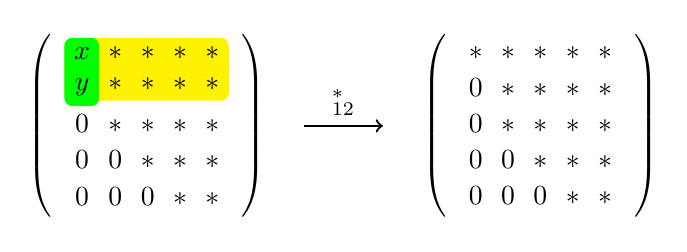
\begin{tikzpicture}
      \node
[matrix of math nodes,left delimiter=(,right delimiter=)] (m)  at (0,0)
{
  x&*&*&*&*\\
  y&*&*&*&*\\
  0&*&*&*&*\\
  0&0&*&*&*\\
  0&0&0&*&*\\
};

\node
[matrix of math nodes,left delimiter=(,right delimiter=)] (r)  at (5,0)
{
  *&*&*&*&*\\
  0&*&*&*&*\\
  0&*&*&*&*\\
  0&0&*&*&*\\
  0&0&0&*&*\\
};

\draw[->,thick] (2,0) -- node[above] {$\matg_{12}^*\matH$} (3,0);

\begin{pgfonlayer}{bg}
  \node[fit={(m-1-1.north west) (m-2-5.south east)},fill=yellow,inner sep=0,rounded corners=1mm]{};
  \node[fit={(m-1-1.north west) (m-2-1.south east)},fill=green,inner sep=0,rounded corners=1mm]{};
\end{pgfonlayer}

;
    \end{tikzpicture}}

  \item Do the same with the second and third rows.

    {\small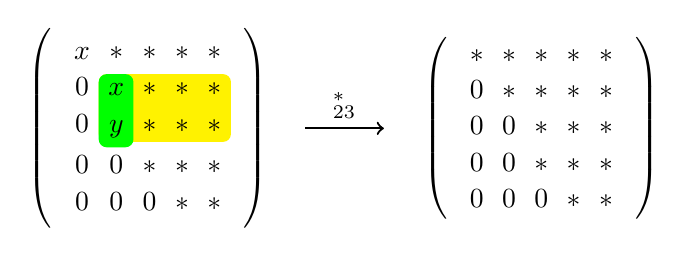
\begin{tikzpicture}
        \matrix
[matrix of math nodes,left delimiter=(,right delimiter=)] (m)
{
  x&*&*&*&*\\
  0&x&*&*&*\\
  0&y&*&*&*\\
  0&0&*&*&*\\
  0&0&0&*&*\\
};

\node
[matrix of math nodes,left delimiter=(,right delimiter=)] (r)  at (5,0)
{
  *&*&*&*&*\\
  0&*&*&*&*\\
  0&0&*&*&*\\
  0&0&*&*&*\\
  0&0&0&*&*\\
};

\draw[->,thick] (2,0) -- node[above] {$\matg_{23}^*\matH$} (3,0);

\begin{pgfonlayer}{bg}
  \node[fit={(m-2-2.north west) (m-3-5.south east)},fill=yellow,inner sep=0,rounded corners=1mm]{};
  \node[fit={(m-2-2.north west) (m-3-2.south east)},fill=green,inner sep=0,rounded corners=1mm]{};
\end{pgfonlayer}
;
      \end{tikzpicture}}

    {\small\begin{tikzpicture}
        \input{fig/hessenberg-givens-3};
      \end{tikzpicture}}

    Note that columns with two zero entries remain unchanged and will not have to be processed.
  \item Now the matrix is upper triangular and the transformation was
    \begin{gather*}
      \matq^* = \givens_{34}^*\givens_{23}^*\givens_{12}^*.
    \end{gather*}

  \item When we go back, we apply Givens rotations from the right, thus affecting columns of the matrices.

    {\footnotesize\begin{tikzpicture}\input{fig/hessenberg-givens-4};\end{tikzpicture}
        \begin{tikzpicture}\input{fig/hessenberg-givens-5};\end{tikzpicture}
        \begin{tikzpicture}\input{fig/hessenberg-givens-6};\end{tikzpicture}
        \begin{tikzpicture}\input{fig/hessenberg-givens-6-result};\end{tikzpicture}}
  \end{enumerate}
\end{example}

\begin{Algorithm*}{Hessenberg-qr-2}{Implicit Hessenberg QR step}
  \begin{algorithmic}[1]
    \Require $\matH\in\Cnn$ in Hessenberg form
    \State $\givens_{1,2} \gets$ Givens rotation for $h_{11},h_{21}$
    \State $\matH \gets \givens^*_{1,2}\matH \givens_{1,2}$
    \For{$k=2,\dots,n-1$}
    \State $\givens_{k,k+1} \gets$ Givens rotation for $h_{k,k-1},h_{k+1,k-1}$
    \State $\matH \gets \givens^*_{k,k+1}\matH \givens_{k,k+1}$
    \EndFor
  \end{algorithmic}
\end{Algorithm*}

\begin{example}
  At the example of a 4-by-4-matrix, we show how this algorithm works.
  \begin{enumerate}
  \item Apply a Givens rotation from the left which eliminates the value $Y$ from the matrix. It affects the two top rows. By
    applying the Givens rotation from the left an additional non zero entry below the subdiagonal is created.

    {\small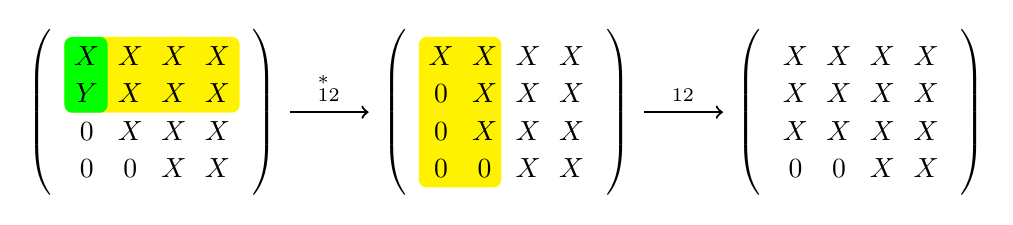
\begin{tikzpicture}
      \node
[matrix of math nodes,left delimiter=(,right delimiter=)] (m)  at (0,0)
{
  X&X&X&X\\
  Y&X&X&X\\
  0&X&X&X\\
  0&0&X&X\\
};

\node
[matrix of math nodes,left delimiter=(,right delimiter=)] (r)  at (4.5,0)
{
  X&X&X&X\\
  0&X&X&X\\
  0&X&X&X\\
  0&0&X&X\\
};
\node
[matrix of math nodes,left delimiter=(,right delimiter=)] (e)  at (9,0)
{
  X&X&X&X\\
  X&X&X&X\\
  X&X&X&X\\
  0&0&X&X\\
};

\draw[->,thick] (1.75,0) -- node[above] {$\matg_{12}^*\matH$} (2.75,0);
\draw[->,thick] (6.25,0) -- node[above] {$\matH \matg_{12}$} (7.25,0);

\begin{pgfonlayer}{bg}
  \node[fit={(m-1-1.north west) (m-2-4.south east)},fill=yellow,inner sep=0,rounded corners=1mm]{};
  \node[fit={(m-1-1.north west) (m-2-1.south east)},fill=green,inner sep=0,rounded corners=1mm]{};
  \node[fit={(r-1-1.north west) (r-4-2.south east)},fill=yellow,inner sep=0,rounded corners=1mm]{};
\end{pgfonlayer}

;
    \end{tikzpicture}}
\item Apply a Givens rotation from the left to restore Hessenberg form of the first column.
  
    {\small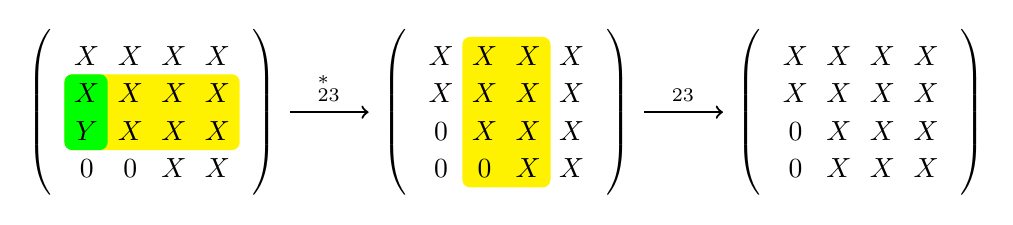
\begin{tikzpicture}
        
\node
[matrix of math nodes,left delimiter=(,right delimiter=)] (m)  at (0,0)
{
  X&X&X&X\\
  X&X&X&X\\
  Y&X&X&X\\
  0&0&X&X\\
};

\node
[matrix of math nodes,left delimiter=(,right delimiter=)] (r)  at (4.5,0)
{
  X&X&X&X\\
  X&X&X&X\\
  0&X&X&X\\
  0&0&X&X\\
};
\node
[matrix of math nodes,left delimiter=(,right delimiter=)] (e)  at (9,0)
{
  X&X&X&X\\
  X&X&X&X\\
  0&X&X&X\\
  0&X&X&X\\
};

\draw[->,thick] (1.75,0) -- node[above] {$\matg_{23}^*\matH$} (2.75,0);
\draw[->,thick] (6.25,0) -- node[above] {$\matH \matg_{23}$} (7.25,0);

\begin{pgfonlayer}{bg}
  \node[fit={(m-2-1.north west) (m-3-4.south east)},fill=yellow,inner sep=0,rounded corners=1mm]{};
  \node[fit={(m-2-1.north west) (m-3-1.south east)},fill=green,inner sep=0,rounded corners=1mm]{};
  \node[fit={(r-1-2.north west) (r-4-3.south east)},fill=yellow,inner sep=0,rounded corners=1mm]{};
\end{pgfonlayer}

;
      \end{tikzpicture}}
    
  \item Do the same with the second column.
    
    {\small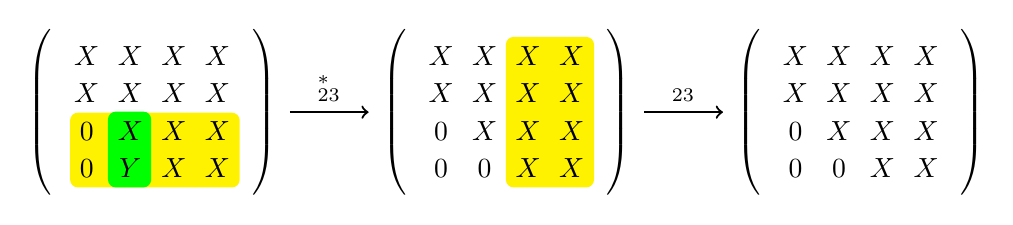
\begin{tikzpicture}
        \node
[matrix of math nodes,left delimiter=(,right delimiter=)] (m)  at (0,0)
{
  X&X&X&X\\
  X&X&X&X\\
  0&X&X&X\\
  0&Y&X&X\\
};

\node
[matrix of math nodes,left delimiter=(,right delimiter=)] (r)  at (4.5,0)
{
  X&X&X&X\\
  X&X&X&X\\
  0&X&X&X\\
  0&0&X&X\\
};
\node
[matrix of math nodes,left delimiter=(,right delimiter=)] (e)  at (9,0)
{
  X&X&X&X\\
  X&X&X&X\\
  0&X&X&X\\
  0&0&X&X\\
};

\draw[->,thick] (1.75,0) -- node[above] {$\matg_{23}^*\matH$} (2.75,0);
\draw[->,thick] (6.25,0) -- node[above] {$\matH \matg_{23}$} (7.25,0);

\begin{pgfonlayer}{bg}
  \node[fit={(m-3-1.north west) (m-4-4.south east)},fill=yellow,inner sep=0,rounded corners=1mm]{};
  \node[fit={(m-3-2.north west) (m-4-2.south east)},fill=green,inner sep=0,rounded corners=1mm]{};
  \node[fit={(r-1-3.north west) (r-4-4.south east)},fill=yellow,inner sep=0,rounded corners=1mm]{};
\end{pgfonlayer}

;
      \end{tikzpicture}}
    Note that columns with two zero entries remain unchanged and will not have to be processed.
  \end{enumerate}
\end{example}

\begin{remark}
  This algorithm is called \define{bulge chasing} with the following
  image in mind. After the application of the first rotation, there is
  a bulge protruding down from the Hessenberg form in the furst
  column. This bulge is then ``chased'' down row by row until it
  leaves the matrix at the bottom.
\end{remark}

\begin{Definition}{hessenberg-unreduced}
  A Hessenberg matrix is called \define{unreduced} if all entries on
  the first subdiagonal are nonzero. It is called \define{reduced}
  otherwise.
\end{Definition}

\begin{todo}
  In the next semester, use $\parallel$!
\end{todo}

\begin{Theorem*}{implicit-Q}{Implicit Q Theorem}
  Let $\mata\in\Cnn$ arbitrary, let $\matq,\matv\in\Cnn$ unitary such that
  \begin{gather}
    \matq^*\mata\matq = \matH,\qquad \matv^*\mata\matv = \matg,
  \end{gather}
  where $\matH$ and $\matg$ are Hessenberg matrices. Let $k$ denote
  the smallest integer such that $h_{k+1,k} = 0$, or $k=n$ if $\matH$
  is unreduced. Assume $\vv_1 = e^{i\phi_0}\vq_1$. Then,
  $\vv_j = e^{i\phi_j}\vq_j$ and $\abs{h_{j+1,j}} = \abs{g_{j+1,j}}$
  for $j=1,\dots,k-1$. if $k<n$, then $g_{k+1,k} = 0$.
\end{Theorem*}

\begin{proof}
  We define the matrix $\matw = \matv^*\matq$, which is orthogonal as the product of orthogonal matrices. There holds
  \begin{gather}
    \matg\matw = \matv^*\mata\matv\matv^*\matq = \matv^*\mata\matq
    = \matv^*\matq\matq^*\mata\matq = \matw\matH.
  \end{gather}
  Spelling out column $j$ of this product, we obtain
  \begin{gather}
    \label{eq:qr:implicitq-1}
    \matg\vw_j = \sum_{k=1}^{j+1} h_{kj} \vw_{k}.
  \end{gather}
  We use this equality to show by induction over the columns that the
  entries $w_{ij}$ of $\matw$ are zero for $i>j$. In other words,
  $\matw$ is upper triangular.  For $j=1$, we obtain from the
  orthogonality of $\matq$ and $\matv$ and the parallelity of $\vq_1$
  and $\vv_1$ that $\vw_1 = e^{i\phi} \ve_1$ for some argument $\phi$.

  Now let the statement be proven for all columns of $\matw$ up to
  column $j$. Then, from~\eqref{eq:qr:implicitq-1} we obtain
  \begin{gather}
    h_{j+1,j}\vw_{j+1} = \matg\vw_j - \sum_{k=1}^j h_{kj} \vw_{k}.
  \end{gather}
  For each vector in the sum, there holds $(\vw_{k})_i = 0$ for
  $i>j$. Since $\matg$ is Hessenberg and applied to $\matw_j$, the
  last possibly nonzero entry of the product is in position $j+1$,
  what we wanted to show.

  Since every orthogonal matrix is normal and due to
  \slideref{Problem}{normal-triangular-diagonal} every triangular
  normal matrix is diagonal, the matrix $(\vw_1,\dots,\vw_k)$ is diagonal with
  diaognal entries of the form $w_{jj} = e^{i\phi_j}$ with some
  arguments $\phi_j$. Hence, $\vv_j = e^{-i\phi_j} \vq_j$ for $j=1,\dots,k$.

  There holds for $j<k$
  \begin{gather}
    \abs{h_{j+1,j}} = \abs{\ve_{j+1}^*\matH\ve_j} = \abs{\vq_{j+1}^*\mata\vq_j}
    = \abs{\vv_{j+1}^*\mata\vv_j} = \abs{g_{j+1,j}}.
  \end{gather}

  If $k<n$, that is, $h_{k+1,k}=0$, it remains to show that
  \begin{multline}
    g_{k+1,k} = \ve_{k+1}^*\matg\ve_k = e^{i\phi_k}\ve_{k+1}^*\matg\matw\ve_k
    =  e^{i\phi_k}\ve_{k+1}^*\matw\matH\ve_k\\
    =  e^{i\phi_k}\ve_{k+1}^* \sum_{j=1}^k h_{jk} \matw\ve_j
    =  \sum_{j=1}^k e^{i\phi_*} h_{jk} \ve_{k+1}^* \ve_j = 0.
  \end{multline}
\end{proof}

\begin{Definition}{essentially-equal}
  The \putindex{Implicit Q Theorem} says that two Hessenberg forms of $\mata$ with the same initial reduction vector are \define{essentially equal} in the sense that they only differ by the diagonal scaling $\matg = \matd^{-1}\matH\matd$ where $\matd=\diag(d_1,\dots,d_n)$ matrix with $\abs{d_{i}} = 1$.
\end{Definition}

\begin{Corollary}{Hessenberg-qr-equivalence}
  The two versions of the Hessenberg QR step are essentially equal.
\end{Corollary}

\begin{Problem}{Hessenberg-qr-effort}
  \begin{enumerate}
  \item How many operations do the two versions of the Hessenberg QR step require?
  \item Show that if $\matH$ is Hermitian, the result of the
    Hessenberg QR step is Hermitian as well.
  \end{enumerate}
\end{Problem}

\begin{Corollary}{Hessenberg-qr}
  The complexity of each step of a QR-iteration for Hessenberg matrices is $\bigo(n^2)$. For tridiagonal (complex) symmetric matrices, it is $\bigo(n)$.
\end{Corollary}

\begin{Theorem}{Hessenberg-householder}
  Every matrix $\mata\in\Cnn$ is unitarily similar to a Hessenberg matrix $\matH$, that is,
  \begin{gather}
    \matH = \matq^* \mata \matq.
  \end{gather}
  The matrix $\matq$ can be obtained by $n-2$ \putindex{Householder
    reflection}s.
\end{Theorem}

\begin{Algorithm*}{qr-method}{The QR-Method}
  Compute the spectrum of a matrix $\mata\in\Cnn$ by
  \begin{enumerate}
  \item Use $n-2$ Householder transformations to transform $\mata$ to
    Hessenberg form
    \begin{gather}
     \matH = \matq^*\mata\matq.
   \end{gather}
 \item QR-iteration: let $\matH_{0}=\matH$ and perform the implicit Hessenberg QR step until convergence
 \item Store Householder vectors as well as $r$ and $c$ for each
   Givens rotation \textbf{only} if the eigenvectors are desired in the end.
  \end{enumerate}
\end{Algorithm*}

\begin{Problem}{Hermitian-tridiagonal}
  Show that every (complex) Hermitian matrix is orthogonally similar
  to a symmetric tridiagonal matrix with real entries.
\end{Problem}

\subsection{Deflation and shifts}

\begin{intro}
  The goal of this section is the development and justification of a
  method which accelerates convergence of the QR-iteration and
  reducing the effort at the same time. It is based on shifts, like
  for the simple or inverse power method. But, shifts are much more
  powerful here, since we compute not only ``converging subspace'',
  but also its complement. The presentation follows
  mostly~\cite{GolubVanLoan83}.
\end{intro}

\begin{Theorem}{qr-reduction}
  Let the matrix $\matH^{(k)}\in\Cnn$ in the QR iteration be of the
  form
  \begin{gather}
    \matH^{(k)} =
    \begin{pmatrix}
      \matH_{11} & \mata_{12}\\0 & \matH_{22}
    \end{pmatrix}
  \end{gather}
  with Hessenberg matrices $\matH_{11}\in\C^{p\times p}$,
  $\matH_{22}\in \C^{n-p\times n-p}$ and an arbitrary matrix
  $\mata_{12}\in \C^{p\times n-p}$. Then, the matrix $\matq^{(k)}$
  decouples into two diagonal blocks and $\matH^{(k+1)}$ has the same
  form. Thus, the iteration decouples into two separate iterations. If
  $p=n-1$, then $h_{nn}$ approximates an eigenvalue.
\end{Theorem}

\begin{Algorithm*}{qr-deflation}{Deflation}
  After each step of the shifted QR-iteration monitor the subdiagonal
  elements of $\matH^{(k)}$. Whenever
  \begin{gather}
    \abs{h_{j,j-1}} \le \eps \bigl(\abs{h_{j-1,j-1}}+\abs{h_{jj}}\bigr)
  \end{gather}
  set $h_{j,j-1}=0$.

  If this happens in the last row, consider $h_{nn}=\lambda_n$
  converged and proceed with a matrix of dimension $n-1\times n-1$.

  If this happens in the center of the matrix, proceed with both
  remaining diagonal blocks separately.

  Note that deflation changes the matrix in a ``nonorthogonal'' way
  and thus changes the eigenvalues. Their accuracy will be determined
  by the parameter $\eps$ in the end.
\end{Algorithm*}

\begin{remark}
  The purpose of deflation is removing Schur vectors from the
  iteration. Thus, if one of the Schur vectors for a multiple
  eigenvalue has converged, the remaining iterations will deal with
  reduced multiplicity. Deflation will also help us to deal with the
  requirement that all eigenvalues must have different modulus, but
  this is solved below in combination with shifts.
\end{remark}

\begin{Algorithm*}{shifted-qr-iteration}{QR iteration with shift}
  \begin{algorithmic}[1]
    \Require $\matH_0 in\Cnn$, Hessenberg, unreduced
    \For {$k=1,\ldots$ until convergence}
    \State $\matq_k\matr_k = \matH_{k-1} - \sigma_k\id$\Comment{QR factorization}
    \State $\matH_{k} = \matr_k\matq_k + \sigma_k\id$
    \EndFor
  \end{algorithmic}
  There is an implicit form of the shifted QR step which follows
  exactly the version outlined for the unshifted case.
\end{Algorithm*}

\begin{Lemma}{shifted-qr-similarity}
  The matrices $\matH_k$ generated by the QR iteration with shifts
  admit the recurrence relation
  \begin{gather}
    \matH_k = \matq_k^*\matH_{k-1}\matq.
  \end{gather}
\end{Lemma}  

\begin{proof}
  The proof is almost identical to \slideref{Lemma}{qr-1}. There holds
  \begin{multline}
    \matH_k = \matr_k\matq_k + \sigma_k \id
    = \matq_k^*\matq_k\matr_k\matq_k + \sigma_k \id\\
    =\matq_k^*\left(\matH_{k-1}-\sigma_k\id\right)\matq_k + \sigma_k \id
    =\matq_k^*\matH_{k-1}\matq_k.
  \end{multline}
\end{proof}

\begin{Lemma*}{perfect-shift}{Perfect shift}
  Let $\matH\in\Cnn$ be an unreduced Hessenberg matrix with eigenvalue
  $\sigma$. Let $\matq\matr = \matH - \sigma\id$ be a QR factorization
  and $\widetilde\matH = \matr\matq+\sigma\id$. Then,
  $\tilde h_{n,n-1}=0$ and $\tilde h_{nn} =\sigma$.
\end{Lemma*}

\begin{proof}
  See also~\cite[Theorem 7.5.1]{GolubVanLoan83}.  Since $\matH$ is
  unreduced, its first $n-1$ columns are linearly independent. Hence,
  if $\matq\matr=\matH-\sigma\id$ is a QR factorization, then
  $r_{ii} \neq 0$ for $i=1,\dots,n-1$.

  Since $\matH-\sigma\id$ is singular, we conclude $r_{nn}=0$. Thus,
  the last row of $\matr\matq$ is zero and the statement holds.
\end{proof}

\begin{intro}
  Obviously, if we knew an eigenvalue, we could deflate right
  away. Thus, the next step in the development of the algorithm is the
  determination of a \define{shift strategy} which drives $h_{n,n-1}$
  to zero by approximating the last eigenvalue.

  Such a shift strategy selects a new shift parameter $\sigma_k$ in
  every step of the algorithm. The shift strategies differ in the
  approximation of the eigenvalue which is closest to $h_{nn}$.
\end{intro}

\begin{Example*}{rayleigh-shift}{Rayleigh shift}
  The Rayleigh quotient for the smallest eigenvalue by magnitude
  converges to $h_{nn}$, as
  \begin{gather}
    \ve_n^* H^{(k)} \ve_n = h_{nn}^{(k)}
  \end{gather}
  and $\vq_n$ is orthogonal to all eigenvectors for eigenvalues of
  greater magnitude. Therefore, using $\sigma_k = h_{nn}^{(k)}$ seems
  a good idea, and often is. But it is not reliable, as in the example
  \begin{gather}
    H =
    \begin{pmatrix}
      0 & 1 \\ 1 & 0
    \end{pmatrix}.
  \end{gather}
\end{Example*}

\begin{Definition*}{wilkinson-shift}{Wilkinson shift}
  Let
  \begin{gather}
    \matm =
    \begin{pmatrix}
      h_{n-1,n-1}^{(k)}&h_{n-1,n}^{(k)}\\h_{n,n-1}^{(k)}&h_{nn}^{(k)}
    \end{pmatrix}.
  \end{gather}
  Then, for $\sigma_k$ use the eigenvalue of $\matm$ which is closer
  to $h_{nn}^{(k)}$.
\end{Definition*}

\begin{Remark}{wilkinson-shift}
  The Wilkinson shift is reliable and the $h_{n,n-1}$ and $h_{nn}$
  converge to zero and the smallest eigenvalue by magnitude,
  respectively. They converge at least quadratically and cubically in
  the symmetric case~\cite[Section 8.2]{GolubVanLoan83}.
\end{Remark}

\begin{Example}{wilkinson-failure}
  Consider the orthogonal matrix
  \begin{gather}
    \mata =
    \begin{pmatrix}
      0&0&1\\1&0&0\\0&1&0
    \end{pmatrix}.
  \end{gather}
  The lower right block has a single eigenvalue zero, such that the
  Wilkinson shift and the Rayleigh shift for this matrix are zero. The eigenvalues of $\mata$ are
  \begin{gather}
    \sigma(\mata) = \left\{1, -\tfrac12 \pm \sqrt{\tfrac34}i\right\},
  \end{gather}
  which all have the same modulus. Thus, the algorithm will not converge with either shift.
\end{Example}

\begin{Algorithm}{exceptional-shift}
  If no deflation has ocurred for a given number of iteration steps of
  the shifted QR iteration, the chosen shift strategy has failed.

  In this case, perform a single step with a random shift parameter, a
  so-called \define{exceptional shift}.
\end{Algorithm}

\begin{remark}
  From the necessity to introduce exceptional shifts, we realize that
  a convergence result for the shifted QR iteration is hard to
  obtain. Nevertheless, from the result for the orthogonal subspace
  iteration, we have
  \begin{gather}
    h_{j+1,j}^{(k)} = \bigo \left(\abs*{\frac{\lambda_{j+1}-\sigma}{\lambda_j-\sigma}}^k\right).
  \end{gather}
  Hence, the situation is not hopeless and typically, the algorithm
  converges again after an exceptional shift.

  We will see soon, that the situation is significantly better in the
  case of Hermitian matrices.
\end{remark}

\begin{Algorithm*}{qr-step-deflation}{QR step with deflation}
  In each step of the QR iteration, first set
  \begin{gather}
    h_{i,i-1} = 0, \qquad \text{where}\quad
    \abs{h_{i,i-1}} \le \eps \left(\abs{h_{i,i}}+\abs{h_{i-1,i-1}}_{\vphantom{g}}\right).
  \end{gather}

  Then, partition the matrix
  $\matH$ as
  \begin{gather}
    \matH =
    \begin{pmatrix}
      \matH_{11} & \matH_{12} & \matH_{13} \\
      & \matH_{22} & \matH_{23}\\
      && \matH_{33}
    \end{pmatrix},
  \end{gather}
  where $\matH_{22}\in\R^{q\times q}$ and
  $\matH_{33}\in\R^{p\times p}$ are chosen maximal such that
  $\matH_{33}$ is upper \putindex{triangular} and $\matH_{22}$
  is unreduced.

  The shifted QR step is then applied to $\matH_{22}$ only. If the
  eigenvectors are not computed, even the transformations of
  $\matH_{12}$ and $\matH_{23}$ can be eliminated.
\end{Algorithm*}

\begin{remark}
  When implementing \slideref{Algorithm}{qr-step-deflation}, we have
  to be able to run a QR step on a submatrix. Allocating new memory
  and copying the submatrix should be avoided since it comes at
  considerable cost.

  This means on the other hand, that the matrix $\matH_{22}$ will not
  be stored as a consecutive array of $q\times q$ numbers. Depending
  on whether the entries are sorted in row-major or column-major
  order, there will either be a gap between each consecutive element
  of a column or between the last element of one column and the first
  element of the next.

  Thus, the QR step operations must allow for a \define{stride}
  between rows or columns. This can be achieved either by storing the
  matrix as a sequence of column vectors, or by using strided versions
  of the algorithms.
\end{remark}

\begin{Example*}{daxpy}{DAXPY}
  The BLAS function daxpy computes
  \begin{gather}
    \vx \gets a \vx + \vy.
  \end{gather}
  It has the signature
  \begin{lstlisting}[language=c]
    int daxpy(int N, double A,
              double* X, int INCX,
              double* Y, int INCY);
  \end{lstlisting}
  The values \lstinline!INCX! and \lstinline!INCY! are used to
  implement stride, possibly with different values in both vectors.
\end{Example*}

%%% Local Variables:
%%% mode: latex
%%% TeX-master: "main"
%%% End:


\section{Methods in real arithmetic}
\begin{intro}
  The multiplication of two complex numbers involves four
  multiplications of real numbers. Hence, if $\mata$ is a real matrix,
  we should avoid computing in complex arithmetic.

  This section consists of two parts. First, we study algorithms for
  Hermitian matrices, which are reduced to real tridiagonal
  matrices. Here, we obtain a very fast algorithm with a guaranteed
  convergence result.

  The second part is about nonsymmetric real matrices, where we face
  the challenge that eigenvalues and eigenvectors may be complex.
\end{intro}

\subsection{The real symmetric eigenvalue problem}

\begin{Lemma}{qr-tridiagonal}
  Let $\matt\in\Rnn$ be a real, symmetric, tridiagonal matrix and
  $\matq\matr=\matt$ its QR factorization. Then, $\tilde\matt=\matr\matq$ is also
  symmetric and tridiagonal. Furthermore, $\matr$ is zero except for
  its main and the first two upper diagonals.

  The same holds for the shifted version with $\sigma\in\R$,
  \begin{gather}
    \matq\matr = \matt-\sigma\id,\qquad \tilde\matt = \matr\matq+\sigma\id.
  \end{gather}
\end{Lemma}

\begin{proof}
  See homework.
\end{proof}

\begin{Remark}{tridiagonal-storage}
  While the mathematical structure of a tridiagonal matrix is that of
  a matrix with its multiplication properties and QR factorization and
  so on, its storage structure consists of two vectors, a diagonal
  vector $\va\in\R^n$ and the upper and lower diagonal
  $\vb\in\R^{n-1}$. Any efficient implementation of the tridiagonal QR
  iteration must use such a reduced storage structure.
\end{Remark}

\begin{Lemma*}{perfect-shift-sym}{Perfect shift}
  Let $\matt\in\Rnn$ be an unreduced, symmetric, tridiagonal matrix,
  $\sigma\in\sigma(\matt)$, and $\matq\matr=\matt-\sigma\id$ the
  shifted QR factorization. Then, $r_{nn}=0$. Furthermore, the last
  column of $\tilde\matt = \matr\matq+\sigma\id$ is equal to
  $\sigma\ve_n$.
\end{Lemma*}

%  \begin{todo}
%\begin{proof}
%  If $\matt$ is unreduced, the first $n-1$ columns of
%  $\matt-\sigma\id$ are linearly independent for any $\sigma$.
%\end{proof}
%  \end{todo}

\begin{Remark*}{real-symmetric-qr}{QR-Iteration for real, symmetric matrices}
  In this case, many things simplify
  \begin{enumerate}
  \item Hessenberg form is tridiagonal
  \item The Schur canonical form is
    \begin{gather}
      \mata = \matq^T\matd\matq
    \end{gather}
    with a real, diagonal matrix $\matd$
  \item QR factorization uses $\bigo(n)$ operations and $\matr$
    consists only of the main diagonal and one upper diagonal.
  \end{enumerate}
  Accumulating the matrix $\matq$ still needs $\bigo(n^2)$ operations and should be avoided!
\end{Remark*}

\begin{Algorithm*}{qr-explicit-shift}{QR iteration with explicit shift}
  \begin{algorithmic}[1]
    \Require $\mata\in\Rnn$ symmetric
    \State $\matt_0 = \matq_0^*\mata\matq_0$\Comment{tridiagonal}
    \For {$k=1,\ldots$ until convergence}
    \State $\matq_k\matr_k = \matt_{k-1} - \sigma_k\id$\Comment{QR factorization}
    \State $\matt_{k} = \matr_k\matq_k + \sigma_k\id$
    \EndFor
  \end{algorithmic}
\end{Algorithm*}

\begin{Lemma}{wilkinson-shift}
  Let
  \begin{gather}
    \matt =
    \begin{pmatrix}
      a_1&b_1\\
      b_1&\ddots&\ddots\\
      &\ddots&a_{n-1}&b_{n-1}\\
      &&b_{n-1}&a_n
    \end{pmatrix}.
  \end{gather}
  Then, the \putindex{Wilkinson shift} $\sigma$ can be computed as
  \begin{gather}
    \sigma = a_n + d - \operatorname{sign}(d) \sqrt{d^2+b_{n-1}^2},
    \qquad d=\frac{a_{n-1}-a_n}2.
  \end{gather}
\end{Lemma}

\begin{Algorithm*}{implicit-symmetric-shift}{Symmetric QR step with implicit shift}
  \begin{algorithmic}[1]
    \Require $\matt\in\Rnn$ symmetric, unreduced, tridiagonal; $\sigma\in\R$
    \State Compute $\matg_{12} = \matg_{12}[t_{11}-\sigma,t_{21}]$\Comment{Givens rotation}
    \State $\matt \gets \matg_{12}^T\matt\matg_{12}$
    \For {$k=2,\dots,n-1$} \Comment{Bulge chasing}
    \State $\matg_{k,k+1} = \matg_{k,k+1}[t_{k,k-1},t_{k+1,k-1}]$
    \State $\matt \gets \matg_{k,k+1}^T\matt\matg_{k,k+1}$
    \EndFor
  \end{algorithmic}
\end{Algorithm*}

\begin{Remark}{tridiagonal-bulge}
  Note that there is no storage space for the ``bulge element'' if the
  matrix is stored in the format of two vectors.

  Therefore, the bulge chasing algorithm must store the bulge element
  separately and keep track of its position.
\end{Remark}

% \begin{todo}
%\begin{example}
%    Graphical representation of bulge chasing
%\end{example}
%  \end{todo}

\begin{Theorem}{implicit-symmetric-shift}
  Given $\matt\in\Rnn$ symmetric, unreduced, and tridiagonal. Let
  \begin{gather}
    \matt^{(e)} = \matq^*\matt\matq,
    \qquad
    \matt^{(i)} = \matz^*\matt\matz,
  \end{gather}
  where $\matt_e$ is computed by the QR step with explicit shift and
  $\matz=\matg_1\matg_2\dots\matg_{n-1}$ is the matrix of the QR step
  with implicit shift. Then, there holds
  \begin{xalignat}2
    \vz_1&=\vq_1,\\
    \vz_i&=\pm \vq_i,& i&=2,\dots,n,\\
    \abs{t_{i,i-1}^{(i)}}&=\abs{t_{i,i-1}^{(e)}},& i&=2,\dots,n.
  \end{xalignat}
\end{Theorem}

\begin{proof}
  Without loss of generality, we can assume that the QR factorization
  in the explicit shift step is computed by Givens rotations.  Then,
  the matrices $\matq$ and $\matz$ are both defined as a product of
  Givens rotations $\matg_{12}\matg_{23}\dots\matg_{k-1,k}$, where the
  first column is defined by the first rotation only. And the first
  rotation matrix is the same for both algorithms, such that
  $\vz_1 = \vq_1$. For the remaining results, we can use the
  \putindex{Implicit Q Theorem}.
\end{proof}

\begin{Theorem}{wilkinson-convergence}
  The QR iteration with Wilkinson shift and deflation converges for
  every symmetric, tridiagonal matrix $\mata$.

  Asymptotically, the convergence is quadratic, that is,
  \begin{gather}
    \abs{h_{nn}^{(k+1)} - \lambda_n} \le c \abs{h_{nn}^{(k)} - \lambda_n}^2.
  \end{gather}

  In many cases, it is even cubic.
\end{Theorem}

\begin{proof}
  The proof is straight from the original article by
  Wilkinson~\cite{Wilkinson68}.  Applying Givens rotations
  $\givens_{n-1,n}\dots \givens_{12}$ to the matrix
  $\overline \mata = \mata^{(k)} - \sigma \id$ with diagonal
  $\overline a_j = a_{jj}-\sigma$ and off-diagonal
  $b_j = a_{j-1,j} = a_{j,j-1}$, we obtain
  \begin{gather}
    \matr^{(k)} =
    \begin{pmatrix}
      p_1 & q_1 & r_1 \\
      0 &p_2 & q_2 & r_2 \\
      & 0 & p_3 & q_3 &r_3 \\
      && 0 & p_4 & q_4 & r_4 \\
      &&& \ddots & \ddots & \ddots &\ddots \\
      &&&& 0 & p_{n-1} & q_{n-1} \\
      &&&&& 0 & x_n
    \end{pmatrix},
  \end{gather}
  where with entries generated inductively from $x_1 = \overline a_1$,
  $y_1= \overline b_2$ by
  \begin{xalignat}2
    \label{eq:real:wilkinson:1}
    p_{j-1} &= \sqrt{x_{j-1} +b_{j}}\\
    \label{eq:real:wilkinson:2}
    c_{j} &= \tfrac{x_{j-1}}{p_{j-1}}
    & s_{j} &= \tfrac{-b_{j}}{p_{j-1}}
    \\
    \label{eq:real:wilkinson:3}
    x_j &= c_j \overline a_j - s_j y_{j-1}
    & y_j &= c_j b_{j+1}.
  \end{xalignat}
  Here, $c_j$ and $s_j$ are the cosine and sine from
  $\givens_{j-1,j}$. The elements $q_j$ and $r_j$ do not contribute to
  the argument and are therefore not computed here.

  Computing now the product
  $\mata^{(k+1)} = \matr\givens_{12}^*\dots\givens_{n-1,n}^* +
  \sigma\id$ with entries $\tilde a_{j}$ and $\tilde b_j$, we obtain
  \begin{gather}
    \mata^{(k+1)} =
    \begin{pmatrix}
      \tilde a_1 & \tilde b_2 \\
      \tilde b_2 & \tilde a_2 & \tilde b_3 \\
      & \tilde b_3 & \tilde a_3 & \tilde b_4 \\
      && \tilde b_4 & \tilde a_4 & \tilde b_5 \\
      &&& \ddots & \ddots &\ddots \\
      &&&& \tilde b_{n-1} & \tilde a_{n-1}& \tilde b_n \\
      &&&&&  \tilde b_n & \tilde a_n
    \end{pmatrix},
  \end{gather}
  where
  \begin{xalignat}2
    \label{eq:real:wilkinson:5}
    \tilde a_n &= c_n x_n + \sigma
    & \tilde b_n &= s_n x_n\\
    \label{eq:real:wilkinson:6}
    \tilde b_j &= s_j p_j & j &= 2,\dots,n-1.
  \end{xalignat}

  Since $\sigma$ is a root of t he characteristic polynomial of the
  lower right block, we have for the entries of $\mata^{(k)}-\sigma\id$
  \begin{gather}
    \label{eq:real:wilkinson:4}
    \overline a_{n-1}\overline a_n - b_n^2 = 0,
    \qquad\text{or}\qquad
    \overline a_n = \frac{b_n^2}{\overline a_{n-1}}
  \end{gather}
  Furthermore, since $\sigma$ is the closest eigenvalue to $a_n$, we have
  \begin{gather}
    \label{eq:real:wilkinson:10}
    \abs{\overline a_{n-1}} \ge \abs{b_n}.
  \end{gather}
  We now show that the product $\abs{b_{n-1}^{(k)}b_{n}^{(k)}}$ is
  monotonically decreasing. To this end, we observe
  \begin{align}
    x_n
    &= c_n \overline a_n - s_n y_{n-1}\\
    &= c_n\frac{b_n^2}{\overline a_{n-1}} - s_n c_{n-1} b_n\\
    &= \frac{b_n}{\overline a_{n-1}}
      \left(c_n b_n - s_n c_{n-1} \overline a_{n-1}\right)\\
    &= \frac{b_n}{\overline a_{n-1}}
      \left(s_n x_{n-1} - s_n c_{n-1} \overline a_{n-1}\right)\\
    &= \frac{b_n}{\overline a_{n-1}}
      \left(s_n c_{n-1} \overline a_{n-1} - s_n s_{n-1}y_{n-2}
      - s_n c_{n-1} \overline a_{n-1}\right)\\
    &= - \frac{b_n}{\overline a_{n-1}} s_n s_{n-1}y_{n-2}\\
    &= - \frac{b_n}{\overline a_{n-1}} s_n s_{n-1} c_{n-2} b_{n-1}.
  \end{align}
  Here, we have used the definition of $x_n$ and $x_{n-1}$
  in~\eqref{eq:real:wilkinson:3} in the first and firth line,
  respectively. The definition of $y_{n-1}$ and $y_{n-2}$ in
  equation~\eqref{eq:real:wilkinson:3} was used in the second and
  seventh line, respectively.  In the second line, we also used
  equation~\eqref{eq:real:wilkinson:4}. In the fourth line, we resolve
  both equations in~\eqref{eq:real:wilkinson:2} for $x_{n-1}$ and
  $b_n$ to obtain
  \begin{gather}
    c_n e_n = s_n x_{n-1}.
  \end{gather}

Now that we are looking at the iteration, all variables will be at
step $k$ unless explicitly noted. By~\eqref{eq:real:wilkinson:5},
\begin{gather}
  b_n^{k+1} = s_n x_n
  = - \frac{b_n}{\overline a_{n-1}} s_n^2 s_{n-1} c_{n-2} b_{n-1}.
\end{gather}
Since all other factors are bounded by one, we obtain
\begin{gather}
  \label{eq:real:wilkinson:7}
  \abs*{b_n^{(k+1)}} \le \abs*{b_{n-1}^{(k)}}.
\end{gather}
By~\eqref{eq:real:wilkinson:6} and the definition of $s_{n}$
in~\eqref{eq:real:wilkinson:2}, we have
\begin{gather}
  b_{n-1}^{(k+1)} = s_{n-1} p_{n-1} = \frac{s_{n-1}b_n}{s_n}.
\end{gather}
Hence,
\begin{align}
  \abs*{b_{n-1}^{(k+1)}b_{n}^{(k+1)}}
  &= \abs*{\frac{s_{n-1}b_{n}}{s_n}
    \frac{b_nc_{n-2}s_n^2s_{n-1}b_{n-1}}{\overline a_{n-1}}}\\
  \label{eq:real:wilkinson:8}
  &= \abs*{b_{n-1}^{(k)}b_{n}^{(k)}}\abs*{\frac{b_n}{\overline a_{n-1}}}
    \abs*{c_{n-2}s_{n-1}^2s_n}\\
  \label{eq:real:wilkinson:9}
    &\le \abs*{b_{n-1}^{(k)}b_{n}^{(k)}}.
\end{align}
Thus, the sequence $\abs{b_{n-1}^{(k)}b_{n}^{(k)}}$ is monotonically
decreasing and, since it is bounded from below, convergent.
Next, we rule out the case where the limit is nonzero. Let
us make this assumption and derive a contradiction. We have
\begin{gather}
  \lim_{k\to\infty}
  \frac{\abs*{b_{n-1}^{(k+1)}b_{n}^{(k+1)}}}%
  {\abs*{b_{n-1}^{(k)}b_{n}^{(k+1)}}}
  = 1,
\end{gather}
which by~\eqref{eq:real:wilkinson:8} implies
\begin{gather}
  \abs*{\frac{b_n}{\overline a_{n-1}}}
  \abs*{c_{n-2}}\abs*{s_{n-1}^2}\abs*{s_n} \to 1.
\end{gather}

Since each of these terms is bounded by one, they must converge to one
individually,
\begin{gather}
  \abs*{\frac{b_n}{\overline a_{n-1}}} \to 1,\qquad
  \abs*{c_{n-2}} \to 1,\qquad
  \abs*{s_{n-1}^2} \to 1,\qquad
  \abs*{s_n} \to 1.
\end{gather}
Since the two sines converge to one, the corresponding cosines converge
\begin{gather}
  \abs*{c_{n-1}^2} \to 0,\qquad \abs*{c_n} \to 0.
\end{gather}
Furthermore,
\begin{gather}
  \abs*{s_n} = \frac{b_n^2}{b_n^2+x_n^2} \to 1
\end{gather}
implies $\abs{x_{n-1}} \to 0$ and
\begin{gather}
  0 = \lim x_{n-1}
  = \lim \Bigl(c_{n-1}\overline a_{n-1} - c_{n-2}s_{n-1}b_{n-1}\Bigr)
  = 0 - 1\cdot \lim b_{n-1},
\end{gather}
yields the contradiction through $b_{n-1} \to 0$.

Hence, the limit is zero and we observe that for any given $\epsilon$
there will be an index $k$ such that $\abs{b_{n-1}^{(k)}b_{n}^{(k)}}$,
which in turn implies that either $\abs{b_{n}^{(k)}}<\epsilon$ or
$\abs{b_{n-1}^{(k)}}<\epsilon$. In the second case, we
apply~\eqref{eq:real:wilkinson:6} to deduce that
$\abs{b_{n}^{(k+1)}}<\epsilon$. In both cases, we reach a regime where
the proof of quadratic convergence below will apply.

Now we tend to the second part of the theorem, namely asymptotic
quadratic convergence. To this end, we assume that the iteration has yielded a matrix
\begin{gather}
  \mata^{(k)} =
  \begin{pmatrix}
    \matb &
    \begin{matrix}
      0\\ \epsilon
    \end{matrix}
    \\
    \begin{matrix}
      0 & \epsilon
    \end{matrix}
    & \frac{\epsilon^2}{\overline a_{n-1}}
  \end{pmatrix}
  =
  \begin{pmatrix}
    \matb&\\&\frac{\epsilon^2}{\overline a_{n-1}}
  \end{pmatrix}
  +
  \begin{pmatrix}
    \\
    &&\epsilon\\
    &\epsilon
  \end{pmatrix}
  .
\end{gather}
Hence, we can use the Bauer-Fike theorem and its
~\slideref{Corollary}{conditioning-eigenvalues-normal} to estimate the
eigenvalue $\lambda_1,\dots,\lambda_n$ of $\mata^{(k)}$ which are also
the eigenvalues of $\mata$. Let $\mu_1,\dots,\mu_{n-1}$ be the
eigenvalues of $\matb$. Then, there is an ordering such that
\begin{gather}
  \begin{aligned}
  \abs*{\lambda_i-\mu_i} & \le \epsilon & i&=1,\dots,n-1\\
  \abs*{\lambda_n - \tfrac{\epsilon^2}{\overline a_{n-1}}} &\le\epsilon.
  \end{aligned}
\end{gather}
All eigenvalues of an unreduced Hessenberg matrix are simple, hence
there is a gap between $\lambda_n$ and all other eigenvalues of
$\mata$, say $\abs{\lambda_i-\lambda_n}\ge \delta$.  Since
\begin{gather}
  \mu_i = \mu_i = \lambda_i+\lambda_i-\lambda_n+\lambda_n
  -\tfrac{\epsilon^2}{\overline a_{n-1}}+\tfrac{\epsilon^2}{\overline a_{n-1}},
\end{gather}
there holds
\begin{align}
  \abs*{\mu_i}
  &\ge \abs*{\lambda_i-\lambda_n} - \abs*{\mu_i-\lambda_i}
    - \abs*{\lambda_n - \tfrac{\epsilon^2}{\overline a_{n-1}}}
    - \abs*{\tfrac{\epsilon^2}{\overline a_{n-1}}}\\
  &\ge \delta - \epsilon - \epsilon -\epsilon = \delta-3\epsilon.
\end{align}
We apply QR factorization to $\mata^{(k)}$ to obtain
$\mata^{(k+1)}$. Before the last givens rotation, the matrix is
\begin{gather}
  \begin{pmatrix}
    \ddots&\ddots&\\
    * & x_{n-1} & \epsilon c_{n-1}\\
    & \epsilon & \tfrac{\epsilon^2}{\overline a_{n-1}}
  \end{pmatrix},
\end{gather}
where by \slideref{Lemma}{tridiagonal-rnn} $\abs{x_{n-1}} \ge \delta-3\epsilon$. Since
\begin{gather}
  \abs{s_n} = \frac{\epsilon}{\sqrt{x_{n-1}^2+\epsilon^2}} \le \frac{\epsilon}{\delta-3\epsilon},
\end{gather}
we conclude
\begin{align}
  \abs*{b_n^{k+1}}
  &= \left(\frac{\epsilon^2}{\overline a_{n-1}} - \epsilon c_{n-1}s_n \right) s_n\\
  &\le \frac{\epsilon^2}{\overline a_{n-1}} \frac{\epsilon}{\delta-3\epsilon}
    + \frac{\epsilon^3}{(\delta-3\epsilon)^2}.
\end{align}
The second term behaves like $\epsilon^3$ as $\epsilon\to0$. For the
first term, we can use~\eqref{eq:real:wilkinson:10} to bound
$\abs{\overline a_{n-1}}\ge\epsilon$ and thus get a term behaving like
$\epsilon^2$, which is the statement of the theorem. On the other
hand, this is not, what is observed when the algorithm is used. The
reason for this discrepancy lies in the fact that the
estimate~\eqref{eq:real:wilkinson:10} is too pessimistic and that the
Wilkinson shift approximates $a_n$, not $a_{n-1}$. But then,
$\abs{\overline a_{n-1}}$ is bounded from below independent of
$\epsilon$. Unfortunately, this behavior cannot be guaranteed.
\end{proof}

\begin{Lemma}{tridiagonal-rnn}
  Let $\mata\in\Rnn$ be symmetric and tridiagonal. If
  $\matq\matr=\mata$ is its QR factorization, then there holds
  \begin{gather}
    \abs{r_{nn}} \ge \min_{\lambda\in\sigma(\mata)} \abs{\lambda}.
  \end{gather}
\end{Lemma}

\begin{proof}
  There holds
  \begin{gather}
    \abs*{r_{nn}} = \norm*{\matr^*\ve_n}_2 = \norm*{\mata\matq^*\ve_n}_2.
  \end{gather}
  Since by \slideref{Theorem}{minmax}
  \begin{gather}
    \min_{\lambda\in\sigma(\mata)}\abs*{\lambda}
    = \min_{\norm{\vx}=1} \norm{\mata\vx},
  \end{gather}
  we immediately conclude the result.
\end{proof}
  
%%%%%%%%%%%%%%%%%%%%%%%%%%%%%%%%%%%%%%%%%%%%%%%%%%%%%%%%%%%%%%%%%%%%%%
\subsection{The eigenvalue problem for nonsymmetric real matrices}
%%%%%%%%%%%%%%%%%%%%%%%%%%%%%%%%%%%%%%%%%%%%%%%%%%%%%%%%%%%%%%%%%%%%%%

\begin{Theorem*}{real-schur-form}{The real Schur form}
  For every matrix $\mata\in \Rnn$ there is an orthogonal matrix
  $\matq\in\Rnn$ and a matrix $\matr\in\Rnn$ such that
  \begin{gather}
    \mata = \matq\matr\matq^*,
    \qquad
    \matr =
    \begin{pmatrix}
      R_{11} &* & *&*\\
      &R_{22}&*&*\\
      &&\ddots&*\\
      &&& R_{jj}
    \end{pmatrix},
  \end{gather}
  where the diagonal blocks are either of dimension one containing the
  real eigenvalues or of dimension 2 for complex conjugate eigenvalue
  pairs. The latter correspond to scaled rotation matrices with the
  according eigenvalue pair.
\end{Theorem*}

\begin{intro}{double-shift}
  When applying the QR step with Wilkinson shift, the shift parameter
  might be complex, thus leading to a bad approximation and
  consequently to slow convergence. Therefore, we have to circumvent
  this situation and find a working method in real arithmetic.
%  Using double shifts, the QR-iteration can be made to converge to the
%  real Schur form using double shifts in real arithmetic. This method
%  is also known as the \define{Francis QR step}~\cite[Algorithm
%  7.5-1]{GolubVanLoan83}.
\end{intro}

\begin{Algorithm*}{double-shift-step}{Explicit double-shift QR step}
  \begin{algorithmic}[1]
    \Require $\matH\in\Rnn$ Hessenberg form, $\sigma_1,\sigma_2\in\C$ shifts
    \State $\matq_1\matr_1 \gets \matH - \sigma_1\id$ \Comment{QR factorization}
    \State $\matH_1 \gets \matr_1\matq_1 + \sigma_1\id$
    \State $\matq_2\matr_2 \gets \matH_1 - \sigma_2\id$ \Comment{QR factorization}
    \State $\matH_2 \gets \matr_2\matq_2 + \sigma_2\id$
  \end{algorithmic}
\end{Algorithm*}

\begin{Remark}{explicit-double-shift-no}
  The explicit double-shift QR step is prone to introduce imaginary
  parts into the matrices due to roundoff errors.

  Never implement the explicit double step! We only introduced it to
  develop the algorithm.
\end{Remark}

\begin{Lemma}{double-shift-matrix}
  Let $\sigma_1,\sigma_2\in\C$ be the eigenvalues of the $2\times2$-matrix
  \begin{gather}
    \matg =
    \begin{pmatrix}
      h_{n-1,n-1}&h_{n-1,n}\\h_{n,n-1}&h_{n,n}
    \end{pmatrix}.
  \end{gather}
  Then, the unitary matrices $\matq_1,\matq_2$ of the double shift
  algorithm with shifts $\sigma_1,\sigma_2$ can be chosen such that
  $\matz = \matq_1\matq_2$ and thus $\matH_2 = \matz^T\matH\matz$ are
  real matrices in exact arithmetic.
\end{Lemma}

\begin{proof}
  First, we realize (homework) that
  \begin{gather}
    \matq_1\matq_2\matr_2\matr_1 = \matm = (\matH-\sigma_1\id)(\matH-\sigma_2\id).
  \end{gather}
  Hence,
  \begin{gather}
    \matm = \matH^2-s\matH+t\id,
  \end{gather}
  where
  \begin{gather}
    \begin{aligned}
      s &= \sigma_1+\sigma_2 = \operatorname{tr}(\matg)&\in&\R,\\
      t &= \sigma_1\sigma_2 = \det(\matg)&\in&\R.
    \end{aligned}
  \end{gather}
  Thus, $\matm\in\Rnn$. Since there is a real QR factorization of
  $\matm$, we can choose $\matz = \matq_1\matq_2\in\Rnn$. Thus, we
  conclude
  \begin{gather}
    \matH_2 = \matq_2^*\matH_1\matq_2 = (\matq_1\matq_2)^*\matH(\matq_1\matq_2) = \matz^T\matH\matz.
  \end{gather}
\end{proof}

\begin{remark}
  The explicit double step has several drawbacks. First, the algorithm
  must choose $\matq_1$ and $\matq_2$ such that their product is
  real. But then, roundoff errors will cause imaginary contributions
  in the result of the double step.

  We could also explicitly compute $\matm$ and then $\matz$ by real QR
  factorization. But here, we need a matrix vector product with
  $\bigo(n^3)$ operations.
\end{remark}

\begin{Theorem}{implicit-double-shift}{Implicit double-shift}
  The following QR step is essentially equivalent to the explicit double-shift:
  \begin{enumerate}
  \item Compute the first column of $\vm_1$ of $\matm$.
  \item Compute a Householder matrix $\matq_0$ such that $\matq_0\vm_1$ is a multiple of $\ve_1$.
  \item Compute Householder matrices $\matq_1,\dots,\matq_{n-2}$ such
    that for $\matp = \matq_0\dots\matq_{n-2}$ there holds
    \begin{enumerate}
    \item $\matp^T\matH\matp$ is a Hessenberg matrix
    \item The first columns of $\matp$ and of $\matz = \matq_1\matq_2$
      of the explicit shift algorithm coincide.
    \end{enumerate}
  \end{enumerate}
\end{Theorem}

\begin{Algorithm*}{francis-qr-step}{Francis QR Step}
  \begin{algorithmic}[1]
    \Require \( \matH \in \Rnn\) unreduced Hessenberg Form
    \State \( s \gets \operatorname{tr}(\matH_{n-1:n, n-1:n})\)
    \State \( t \gets \det(\matH_{n-1:n, n-1:n})\)
    \State \(\vw \gets \left(\matH^2 - s \matH + t \id\right)_{:,1}\)
    \State \(\matq \gets \mathtt{Householder\_Matrix}(\vw)\)
    \State \( \matH \gets \matq^\mathsf{T} \matH \matq\)
    \For{\(i = 1, \ldots , n-2\)}
      \State \(\matq \gets \mathtt{Householder\_Matrix}(\matH_{i+1:n,i})\)
      \State \( \matH \gets \matq^\mathsf{T} \matH \matq\)
    \EndFor
  \end{algorithmic}
\end{Algorithm*}

\begin{remark}
  The matrix $\matm$ in the double shift algorithm is not Hessenberg,
  but it has two nonzero lower diagonals. Thus, we use Householder
  reflection for $\matq_0$ and eliminate $h_{21}$ and $h_{31}$. The
  resulting matrix will have an additional entry $h_{31}$.

  The subsequent Householder reflections $\matq_k$ are used to
  eliminate the additional lower diagonal entry $h_{k+2,k}$ in the
  same fashion as the ``bulge chasing'' for the symmetric implicit
  shift. This method is often named \define{Francis QR step} after its
  inventor.
\end{remark}

\begin{Algorithm*}{deflation-francis}{Deflation for Francis QR iteration}
  In each step of the Francis QR iteration, first set
  \begin{gather}
    h_{i,i-1} = 0, \qquad \text{where}\quad
    \abs{h_{i,i-1}} \le \text{tol} (\abs{h_{i,i}}+\abs{h_{i-1,i-1}}).
  \end{gather}

  Then, partition the matrix
  $\matH$ as
  \begin{gather}
    \matH =
    \begin{pmatrix}
      \matH_{11} & \matH_{12} & \matH_{13} \\
      & \matH_{22} & \matH_{23}\\
      && \matH_{33}
    \end{pmatrix},
  \end{gather}
  where $\matH_{22}\in\R^{q\times q}$ and
  $\matH_{22}\in\R^{p\times p}$ are chosen maximal such that
  $\matH_{33}$ is upper \putindex{quasi-triangular} and $\matH_{22}$
  is unreduced.

  The Francis QR step is then applied to $\matH_{22}$ only. If the
  eigenvectors are not computed, even the transformations of
  $\matH_{12}$ and $\matH_{23}$ can be eliminated.
\end{Algorithm*}

\begin{remark}
  Both the symmetric and the unsymmetric algorithms become more
  efficient, if eigenvectors are not computed by accumulating the
  necessary transformations.

  A way around this is the application of the shifted inverse
  iteration with the approximated eigenvalues, which typically
  converges in one step for well-conditioned problems.
\end{remark}


%%% Local Variables:
%%% mode: latex
%%% TeX-master: "main"
%%% End:


\section{Computing eigenvectors}
%\input{orthopoly}

\chapter{Solving Large Sparse Linear Systems}
\label{chap:sparse}

\section{Sparse matrices}

\chapter{Solving Large Sparse Linear Systems}
\label{chap:sparse}

\section{Sparse matrices}

\begin{intro}
  A simple method to approximate the solution to partial differential
  equations is the finite difference method. We provide a short
  introduction sufficient for the purpose in this class in
  Appendix~\ref{sec:fd}.
\end{intro}

\begin{Example}{7-point-stencil}
  Let there be a sequence of points $x_k$, $k=0,\dots,n$ such that
  $x_k-x_{k-1} = h$ and an approximating function $u_k = u(x_k)$. The
  second derivative of a function $u(x)$ in a point $x_k$ in the
  interior can be approximated by the 3-point stencil
  \begin{gather}
    u''(x_k) = \Delta_h^2 u(x_k) = - \frac{2 u_k - u_{k-1} - u_{k+1}}{h^2}.
  \end{gather}
  This can be generalized to the Laplacian in two dimensions by the \define{5-point stencil}
  \begin{gather}
    \Delta u_{ij} = -\frac{4 u_{ij}- u_{i-1,j} - u_{i+1,j}- u_{i,j-1} - u_{i,j+1}}{h^2},
  \end{gather}
  and to three dimensions by the \define{7-point stencil}
  \begin{multline}
    \Delta u_{ijk} = \tfrac{-1}{h^2}\Bigl(6 u_{ij}
    - u_{i-1,j,k} - u_{i+1,j,k}
    \\
    - u_{i,j-1,k} - u_{i,j+1,k}
    - u_{i,j,k-1} - u_{i,j,k+1}\Bigr).
  \end{multline}
\end{Example}

\begin{Example*}{page-rank}{The PageRank Algorithm}
  The page rank of a web page is computed from the Google Matrix
  \begin{gather}
    \matp = d (\matl+\vw \mathbf 1^T) + \tfrac{(1-d)}{n} \id,
  \end{gather}
  where $d \in (0,1)$ is a damping parameter, $\mathbf 1^T = (1,\dots,1)$,
  \begin{gather}
    l_{ij} =
    \begin{cases}
      \nicefrac1{c_i} & \text{if $i$ links to $j$}\\0&\text{else} 
    \end{cases},
    \qquad
    w_i =
    \begin{cases}
      1 &\text{if } c_i=1\\
      0&\text{else}
    \end{cases},
  \end{gather}
  and $c_i$ is the number of links from page $i$.

  The number of web pages is estimated at 4.86 billion pages\footnote{\url{https://www.worldwidewebsize.com/}}.
\end{Example*}

\begin{intro}
  A simple method to approximate the solution to partial differential
  equations is the finite difference method. We provide a short
  introduction sufficient for the purpose in this class in
  Appendix~\ref{sec:fd}.
\end{intro}

\begin{Example}{7-point-stencil}
  Let there be a sequence of points $x_k$, $k=0,\dots,n$ such that
  $x_k-x_{k-1} = h$ and an approximating function $u_k = u(x_k)$. The
  second derivative of a function $u(x)$ in a point $x_k$ in the
  interior can be approximated by the 3-point stencil
  \begin{gather}
    u''(x_k) = \Delta_h^2 u(x_k) = - \frac{2 u_k - u_{k-1} - u_{k+1}}{h^2}.
  \end{gather}
  This can be generalized to the Laplacian in two dimensions by the \define{5-point stencil}
  \begin{gather}
    \Delta u_{ij} = -\frac{4 u_{ij}- u_{i-1,j} - u_{i+1,j}- u_{i,j-1} - u_{i,j+1}}{h^2},
  \end{gather}
  and to three dimensions by the \define{7-point stencil}
  \begin{multline}
    \Delta u_{ijk} = \tfrac{-1}{h^2}\Bigl(6 u_{ij}
    - u_{i-1,j,k} - u_{i+1,j,k}
    \\
    - u_{i,j-1,k} - u_{i,j+1,k}
    - u_{i,j,k-1} - u_{i,j,k+1}\Bigr).
  \end{multline}
\end{Example}

\begin{Definition}{sparse-matrix}
  We call a matrix \textbf{sparse}\index{sparse matrix} in strict
  sense, if the number of nonzero entries is much less than the total
  number of entries, typically $\bigo(n)$ instead of $\bigo(n^2)$. The
  distribution of nonzero entries is called \define{sparsity pattern}.

  More broadly, a sparse matrix has the property that its application
  to a vector requires considerably less than $n^2$, typically
  $\bigo(n)$ operations. It also can be stored with considerably less
  than $n^2$ floating point numbers.
\end{Definition}

\begin{Example*}{csr}{Compressed row storage (CSR)}
  A sparse matrix can be stored using two integer fields defining the
  sparsity pattern and a field of floating point values for its
  entries. Let \lstinline!n! be the dimension of the matrix and
  \lstinline!n_nonzero! the total number of nonzero entries.
  \begin{lstlisting}[language=Python]
    import numpy as np
    row_start = np.empty(n, dtype=np.uint)
    column = np.empty(n_nonzero, dtype=np.uint)
    entries = np.emtpy(n_nonzero, dtype=np.double)
  \end{lstlisting}

  The operation $\vy=\mata\vx$ is then implemented as
  \begin{lstlisting}[language=Python]
    for i in range(0,n):
    y[i] = 0.
    for j in range (row_start[i],row_start[i+1):
      y[i] += entries[j]*x[column[j]]
  \end{lstlisting}  
\end{Example*}

\begin{Remark}{algorithmic-matrix}
  In cases where the sparsity pattern and the entries of a matrix are
  known at compile time, a compressed stored matrix can be substituted
  by an algorithm performing the multiplication.

  Thus, we start viewing matrices more as linear operators than as
  rectangular schemes of numbers.

  Such algorithms are of high importance on modern hardware, where the
  time and also the energy cost of computations is much lower than of
  moving data from memory.
\end{Remark}

\begin{Example}{sparse-computation-memory}
  The matrix of the 7-point stencil on a grid of $N=n^3$ points has
  dimension $N$. For $n=100$, this is $N=10^6$. The whole matrix has
  $N^2=10^{12}$ entries, but only $7N \approx 10^7$ are nonzero.
  \begin{enumerate}
  \item Storing the full matrix in double precision requires
    \begin{gather}
     8\cdot 10^{12}\text{B} \approx 10\text{TB}. 
    \end{gather}
    Storing relevant information in
    CSR requires
    \begin{gather}
      12\cdot7\cdot 10^6\text{B} \approx 100\text{MB}.
    \end{gather}
  \item On a hypothetical CPU with $10^9$ multiplication/additions per second, multiplying a vector with this matrix takes
    \begin{gather}
      \text{Full: } 1000\text{sec} \approx 20\text{min},
      \qquad
      \text{CSR: } 7\text{msec}.
    \end{gather}
  \end{enumerate}
\end{Example}

\begin{Example}{sparse-computation-factorization}
  Solving a linear system with the matrix of the 7-point stencil on a $100^3$ grid
  \begin{enumerate}
  \item Full Choleski factorization
    \begin{gather}
      \frac16 \left(100^3\right)^3\text{flops}\approx 10^{17}\text{flops}
      \simeq 10^8\text{sec} \approx 3\text{yrs.}
    \end{gather}
%    \pause
  \item Banded Choleski factorization
    \begin{gather}
      \frac16 10^{16} \approx 10^{15}\text{flops}
      \simeq 10^6\text{sec} \approx 10\text{d}.
    \end{gather}
%    \pause
  \item Cramer's Rule with Laplace Expansion: $\approx 10^{65,000}$ years.
  \end{enumerate}
\end{Example}


\begin{Theorem*}{von-Neumann-series}{von Neumann series}
  If $\norm{\mata}<1$, then the right hand side of the following
  equation is convergent and
  \begin{gather}
    (\id-\mata)^{-1} = \sum_{k=0}^{\infty} \mata^k.
  \end{gather}
\end{Theorem*}

\begin{Algorithm}{von-Neumann-series}
  An approximative solution to the problem $\mata\vx = \vb$ can
  be obtained from an initial vector $\vx$ by the iteration
  \begin{algorithmic}
    \State $\vy \gets \vx$
    \Repeat
    \State $\vy \gets (\id-\mata) \vy$
    \State $\vx \gets \vx + \vy$
    \Until convergence
  \end{algorithmic}
  This algorithm converges for any initial vector if $\norm{\id-\mata}< 1$.
\end{Algorithm}

\begin{intro}
  While this algorithm serves as a first example that a linear system
  can be solved by successive multiplication with $\mata$, it
  typically slow. Furthermore, most matrices will not admit the
  condition. It is therefore our goal to find more efficient and
  reliable algorithms.
\end{intro}

%%% Local Variables:
%%% mode: latex
%%% TeX-master: "main"
%%% End:


\section{Basic iterative methods}
\input{iterations}

\section{Projection methods}
\begin{Definition}{galerkin-method}
  Let $\mata\in\Rnn$ and $\vb, \vx\in\R^n$ with $\mata\vx=\vb$. Then,
  the vector $\tilde\vx\in\R^n$ is called the \define{Galerkin
    approximation} of $\vx$ in a subspace $K$ orthogonal to a subspace
  $L$, if there holds
  \begin{align}
    \tilde\vx &\in K,\\
    \vb-\mata\tilde\vx &\perp L.
                         \label{eq:proj-it:1}
  \end{align}
  This type of approximation is called \define{Galerkin method}, more
  specifically \define{Ritz-Galerkin method} in the case $K=L$ and
  \define{Petrov-Galerkin method} in the case $K\neq L$.
\end{Definition}

\begin{remark}
  Projection methods are at first hand not iterative, but they produce
  an approximation $\tilde \vx$ in one step. Nevertheless, this
  approximation may not be sufficiently accurate. In this case, we
  have two options:
  \begin{enumerate}
  \item We can enrich the subspaces $K$ and $L$, typically by a
    one-dimensional subspace each, in order to obtain a better
    approximation $\tilde \vx$ in this larger space.
  \item We can rewrite the projection method in an incremental way,
    where the result of a previous step is improved by an update
    obtained from a projection step.
  \end{enumerate}
\end{remark}

\begin{Definition}{projection-step}
  Given a vector $\vx^{(k)}\in\R^n$ and its residual
  $\vr^{(k)}=\vb-\mata\vx^{(k)}$. Then, we say that the vector
  $\vx^{(k+m)}\in\R^n$ is obtained by a \define{projection step}, if
  \begin{gather}
    \vx^{(k+m)} = \vx^{(k)} + \vv,
  \end{gather}
  where after the choice of $m$-dimensional subspaces $K_k$ and $L_k$ the update $\vv$ is
  determined by the condition
  \begin{align}
    \vv &\in K_k\\
    \vr^{(k+m)} \equiv \vr^{(k)} - \mata\vv &\perp L_k.
  \end{align}
  A method of this type is called \define{successive subspace correction} method.
\end{Definition}

\begin{remark}
  The notation $\vx^{(k+m)}$ in the previous definition is quite
  arbitrary and we could have written $\vx^{(k+1)}$ as
  well. Nevertheless, algorithms we will study later have a structure
  where the $m$-dimensional projection step will resemble $m$
  one-dimensional steps, at least from the algorithmic point of
  view. Thus, we adopt the view of a single step in dimension $m$ as
  an $m$-fold step.

  Since most methods determine the update in each step by the same
  algorithm, we will typically only discuss the step from $\vx^{(0)}$
  to $\vx^{(m)}$, thus omitting the index $k$ of the initial vector of
  the step, or discuss a step from $\vx$ to $\tilde\vx$, hence
  omitting indices at all, while keeping in mind that there is an
  iterative procedure in the background.
\end{remark}

\begin{Notation}{incremental}
  We will mostly only consider a single step of the iterative
  projection method. Since the algorithm determining the update
  usually does not vary between steps, we will equivalently describe
  iteration steps as mappings
  \begin{align*}
    \vx^{(k)} &\mapsto \vx^{(k+m)}\\
    \vx^{(0)} &\mapsto \vx^{(m)}\\
    \vx &\mapsto \tilde\vx
  \end{align*}
\end{Notation}

\begin{Definition}{parallel-subspace-correction}
  Given an initial vector $\vx$, a step of the \define{parallel
    subspace correction} method is obtained by choosing $m$ subspaces
  $K_1\dots,K_m$ and $L_1,\dots,L_m$, and computing independently $m$
  update vectors by the projection conditions
  \begin{align}
    \vv_i &\in K_i\\
    \vr_i \equiv \vb-\mata\vx - \mata\vv_i &\perp L_i.
  \end{align}
  The result of the correction step is
  \begin{gather}
    \tilde \vx = \vx + \omega\sum\vv_i,
  \end{gather}
  where $\omega$ is a relaxation parameter chosen to achieve convergence.
\end{Definition}

\begin{Example}{projection-gauss-seidel}
  The Gauss-Seidel and the Jacobi substeps are projection steps with the choice
  \begin{gather}
    K=L=\spann{\ve_i}.
  \end{gather}
  Here, each step of the Jacobi iteration is a parallel subspace
  correction method, while the Gauss-Seidel iteration is a successive
  subspace correction method.
\end{Example}

\begin{proof}
  The condition for the update vector $\vv_i$ is
  \begin{gather}
    \scal(\vb-\mata\vx-\mata\vv_i,\ve_i) = 0,
  \end{gather}
  which, since $\vv_i$ is a multiple of $\ve_i$, translates to
  \begin{gather}
    \vb_i - (\mata\vx)_i - a_{ii}v_i = \vb_i-\sum_{j\neq i} a_{ij}x_j - a_{ii}x_i -a_{ii}v_i.
  \end{gather}
  Hence
  \begin{gather}
    v_i = -x_i + \frac1{a_{ii}} \left(\vb_i - \sum_{j\neq i} a_{ij}x_j\right).
  \end{gather}
  For the parallel subspace correction method, we have for each component independently
  \begin{gather}
    x_i = x_i+v_i = \frac1{a_{ii}} \left(\vb_i - \sum_{j\neq i} a_{ij}x_j\right),
  \end{gather}
  which is equal to the Jacobi step. For the successive subspace
  correction method, we obtain the Gauss-Seidel step by observing that
  the start vector $\vx$ changes in every step.
\end{proof}

\begin{Definition}{projection-method-matrix}
  Let $\matv=(\vv_1,\dots,\vv_m)$ and $\matw=(\vw_1,\dots,\vw_m)$ be bases for
  the subspaces $K$ and $L$, respectively. Then, the solution
  $\vx^{(m)}$ to the projection step is determined by $\vy\in\R^m$ and
  \begin{align}
    \vx^{(m)} &= \vx^{(0)} + \matv\vy\\
    \matw^*\mata\matv \vy &= \matw^* \vr^{(0)}.
  \end{align}
  It is thus obtained by solving an $m$-by-$m$ linear system, called
  the projected system or the \define{Galerkin
    equations}. $\matw^*\mata\matv\in\R^{m\times m}$ is the
  \define{projected matrix}.
\end{Definition}

\begin{proof}
  See \cite[Section 5.1.2]{Saad00}. We observe that the Galerkin condition translates to
  \begin{gather}
    \scal(\vw_i,\vb-\mata\vx^{(0)}-\mata\vv)\qquad i=1,\dots,m,
  \end{gather}
  which we can rewrite as a matrix equation
  \begin{gather}
    \matw^*(\vb-\mata\vx^{(0)}-\mata\vv) = \matw^*\vr^{(0)} -
    \matw^*\mata\matv.
  \end{gather}
  Since we can express $\vv$ in terms of the basis $\matv$, we obtain
  \begin{gather}
    \matw^*\mata\vv = \matw^*\mata\matv\vy,
  \end{gather}
  for some vector $\vy\in\R^m$.
\end{proof}

\begin{Theorem}{projected-invertible}
  Let one of the following conditions hold:
  \begin{enumerate}
  \item $\mata$ is symmetric, positive definite and $L=K$.
  \item $\mata$ is invertible and $L = \mata K$.
  \end{enumerate}
  Then, the projected matrix $\matw^*\mata\matv$ is invertible for any
  bases $\matv$ and $\matw$ of $K$ and $L$, respectively.
\end{Theorem}

\begin{proof}
  First, consider the symmetric, positive definite case. Since $K=L$,
  we can use the same basis $\matw=\matv$  and obtain
  \begin{gather}
    \mata_m = \matv^*\mata\matv,
  \end{gather}
  which inherits the symmetry from $\mata$. Hence, we can estimate its
  lowest eigenvalue by the Rayleigh quotient,
  \begin{multline}
    \lambda_{\text{min}}(\mata_m)
    = \min_{\vy\in\R^m} \frac{\scal(\mata_m\vy,\vy)}{\scal(\vy,\vy)}
    = \min_{\vy\in\R^m} \frac{\scal(\matv^*\mata\matv\vy,\vy)}{\scal(\vy,\vy)}
    \\
    = \min_{\vy\in\R^m} \frac{\scal(\mata\matv\vy,\matv\vy)}{\scal(\vy,\vy)}
    \ge\min_{\vv\in\R^n} \frac{\scal(\mata\vv,\vv)}{\scal(\vv,\vv)}
    \min_{\vy\in\R^m} \frac{\scal(\matv\vy,\matv\vy)}{\scal(\vy,\vy)}.
  \end{multline}
  Both factors are positive, the first by the positive definiteness of
  $\mata$, the second because $\matv$ is a basis. The results holds
  for a different basis $\matw$ on the left, since this corresponds to
  multiplying $\mata_m$ by an invertible matrix from the left.

  If $\mata$ is invertible and $L=\mata K$ we choose
  $\matw=\mata\matv$. Observing that $\mata^*\mata$ is symmetric and
  positive definite, we can apply the previous argument.
\end{proof}

\begin{Theorem}{projection-orthogonal-optimal}
  Let $\mata\in\Rnn$ be symmetric, positive definite. Then,
  $\tilde \vx$ is the result of the orthogonal ($L=K$) projection
  method with previous state $\vx^{(k)}$ if and only if it minimizes
  the \putindex{A-norm} of the error over the space $\vx^{(k)}+K$. Namely, for the
  solution $\vx$ of $\mata\vx=\vb$ there holds
  \begin{gather}
    \norm{\tilde\vx-\vx}_A
    = \min_{\vv\in \vx^{(k)}+K} \norm{\vv-\vx}_A
    = \min_{\vv\in K} \norm{\vv+\vx^{(k)}-\vx}_A.
  \end{gather}
  Here, $\norm\vv_A = \sqrt{\vv^*\mata\vv}$.
\end{Theorem}

\begin{proof}
  We use the definition of the projection step to derive for
  $\tilde \vx = \vx^{(k+m)}$ and any $\vw \in L = K$:
  \begin{align}
    0
    &= \scal(\vr^{(k)} - \mata \vv,\vw)\\
    &= \scal(\vb-\mata\tilde\vx,\vw)\\
    &= \scal(\mata\vx - \mata\tilde\vx,\vw)\\
    &= \scal(\vx-\tilde\vx,\vw)_{\mata}.
  \end{align}
  That is, the error after the projection step is orthogonal to the
  test space $K$ in the $\mata$-inner product. Hence, we can continue
  with a standard proof for the optimality of orthogonal
  projection. We present here the \putindex{variational method} which
  is also used in functional analysis. To this end, we define for
  arbitrary nonzero $\vw\in K$ the function
  \begin{gather}
    F(t) = \tfrac12 \norm{\tilde\vx+t\vw-\vx}_{\mata}^2.
  \end{gather}
  We observe that since $\tilde\vx \in \vx^{(k)}+K$, also
  $\tilde\vx + t \vw \in \vx^{(k)}+K$. Hence, we can replace the
  minimum as one over $\vw$ and $t$.
  
  We observe that if $\tilde\vx$ is a minimizer of the norm, then this
  function has a minimum at $t=0$. Furthermore, if it has a minimimum
  at $t=0$ for all $\vw\in K$, then this implies that $\tilde\vx$ is a
  minimum over $K$. Hence, we have reduced the question to a set of
  one-dimensional minimization problems. We have
  \begin{align}
    F(t) &= \tfrac{t^2}2 \norm{\vw}_{\mata}^2 + t \scal(\tilde\vx-\vx,\vw)
    + \tfrac12 \norm{\tilde\vx-\vx}_{\mata}^2,\\
    F'(t) &= t\norm{\vw}_{\mata}^2 + \scal(\tilde\vx-\vx,\vw)_{\mata},\\
    F''(t) &= \norm{\vw}_{\mata}^2 = \vw^*\mata\vw.
  \end{align}
  These derivatives are also called \define{first variation} and
  \define{second variation} of the minimization problem.
  Necessary and sufficient for a minimum at $t=0$ is $F'(0)=0$ and
  $F''(0)>0$. The latter is due to the positive definiteness of
  $\mata$. The first is fulfilled if
  \begin{gather}
    F'(0) = \scal(\tilde\vx-\vx,\vw)_{\mata} = 0,
  \end{gather}
  which is exactly what we derived for the projection step.
\end{proof}


\begin{Theorem}{projection-oblique-optimal}
  Let $\mata\in\Rnn$ and $L=\mata K$. Then, $\tilde \vx$ is the result
  of the (oblique) projection method with previous state $\vx^{(k)}$
  if and only if it minimizes the Euclidean norm of the residual
  $\vb-\mata\tilde\vx$ over the space $\vx^{(k)}+K$. Namely, there
  holds
  \begin{gather}
    \norm{\vb-\mata\tilde\vx}_2
    = \min_{\vy\in\vx^{(k)}+K} \norm{\vb-\mata\vy}_2
  \end{gather}
\end{Theorem}

\begin{proof}
  We begin as in the previous proof and use the definition of the
  projection step to derive for $\tilde \vx = \vx^{(k+m)}$ and any
  $\mata\vw \in L = \mata K$:
  \begin{align}
    0
    &= \scal(\vr^{(k)} - \mata \vv,\mata\vw)\\
    &= \scal(\vb-\mata\tilde\vx,\mata\vw)\\
    &= \scal(\mata\vx - \mata\tilde\vx,\mata\vw)\\
    &= \scal(\vx-\tilde\vx,\vw)_{\mata^*\mata}.
  \end{align}
  Since $\mata^*\mata$ is positive definite if $\mata$ is nonsingular,
  we can proceed as in the previous theorem, observing that
  \begin{gather}
    \norm{\vb-\mata\tilde\vx}^2 = \scal(\vb-\mata\tilde\vx,\vb-\mata\tilde\vx)
    = \scal(\vx-\tilde\vx,\vx-\tilde\vx)_{\mata^*\mata}.
  \end{gather}
\end{proof}

\begin{Theorem}{projection-1d}
  Any one-dimensional projection method can be characterized by two
  vectors, the \define{search direction} $\vv$ and the test vector
  $\vw$. Then,
  \begin{gather}
    K = \spann{\vv^{(k)}},
    \qquad L = \spann{\vw^{(k)}}.
  \end{gather}
  The new solution is
  \begin{gather}
    \vx^{(k+1)} = \vx^{(k)}+\alpha_k \vv^{(k)},
  \end{gather}
  where
  \begin{gather}
    \label{eq:projection:1d-1}
    \alpha_k = \frac{\scal(\vr^{(k)},\vw^{(k)})}{\scal(\mata\vv^{(k)},\vw^{(k)})}.
  \end{gather}
\end{Theorem}

\begin{proof}
  After choosing the spaces $K$ and $L$, the method is uniquely defined. Since (omitting indices)
  \begin{gather}
    \scal(\vb-\mata\vx - \alpha\mata\vv,\vw) = 0,
  \end{gather}
  we have
  \begin{gather}
    \alpha\scal(\mata\vv,\vw) = \scal(\vr,\vw),
  \end{gather}
  which implies the formula for $\alpha$ if the denominator is nonzero.
\end{proof}

\begin{Definition}{breakdown}
  The computation of the step length in all projection methods
  requires a division as in~\eqref{eq:projection:1d-1}. If the
  denominator is zero, the next step of the method cannot be
  computed. We call this a \define{breakdown} of the method.
  
  Furthermore, this value might be almost zero, which is called a
  \define{near breakdown}. In this case, the next step might be
  computed, but it will suffer from round-off errors.
\end{Definition}

\begin{Algorithm*}{steepest-descent-algol}{The steepest descent method}
  \begin{algorithmic}[1]
    \Require $\mata\in\Rnn$ s.p.d.; $\quad\vx,\vb\in\R^n$
    \State $\vr\gets \vb-\mata\vx$
    \Repeat
    \State $\alpha\gets\frac{\scal(\vr,\vr)}{\scal(\mata\vr,\vr)}$
    \State $\vx \gets \vx + \alpha\vr$
    \State $\vr \gets \vr-\alpha\mata\vr$
    \Until convergence
  \end{algorithmic}
\end{Algorithm*}

\begin{Lemma}{steepest-descent}
  Each step of the steepest descent method computes the minimum of
  $F(\vy) = \frac12\norm{\vy-\vx}_A^2$ along the line from the current
  iterate $\vx^{(k)}$ in direction $\vw = -\nabla F(\vx^{(k)}) = -\vr^{(k)}$.
  Furthermore, there holds
  \begin{gather}
    \vr^{(k+1)} \perp \vr^{(k)}.
  \end{gather}
\end{Lemma}

\begin{proof}
  This result is an immediate consequence of
  \slideref{Theorem}{projection-orthogonal-optimal}. From the proof of
  this theorem, we deduce for any $\vw$
  \begin{gather}
    \nabla F(\vx^{(k)})(\vw) = \scal(\vx^{(k)}-\vx,\vw)_{\mata}
    = -\scal(\vr^{(k)},\vw).
  \end{gather}
  Furthermore, the orthogonality condition of the orthogonal
  projection method implies
  \begin{gather}
    0 = \scal(\vr^{(k+1)},\vw^{(k)}) = -\scal(\vr^{(k+1)},\vr^{(k)}).
  \end{gather}
\end{proof}

\begin{Example}{steepest-descent-10}
  We run the steepest descent method for
  \begin{gather}
    \mata =
    \begin{pmatrix}
      .1 \\&1
    \end{pmatrix},
    \vb =
    \begin{pmatrix}
      0\\0
    \end{pmatrix},
    \vx^{(0)} =
    \begin{pmatrix}
      -10\\1
    \end{pmatrix}.
  \end{gather}
  The iteration history together with  the level sets of $\vx^T\mata\vx$ is
  \begin{center}
    \includegraphics[width=.8\textwidth]{./graph/steepest-descent-10.tikz}
  \end{center}
\end{Example}

\begin{remark}
  In this algorithm, the operation $\mata\vr$ is applied twice. Since
  in most implementations this will be the part with the most
  computational operations, we introduce an auxiliary vector
  $\vp = \mata\vr$, which can be used in lines 3 and 5. At the cost of
  one additional vector, the numerical effort per step is almost
  cut in half.
\end{remark}

\begin{Remark}{convergence-residual}
  The residual $\tilde \vr = \vb - \mata\tilde\vx$ of the current iterate
  $\tilde\vx$ measures the misfit of $\tilde\vx$ in the equation
  $\mata\vx = \vb$. Since the error $\tilde\vx-\vx$ is unknown, we can
  use it as criterion for the accuracy of the current
  solution. Indeed, there holds
  \begin{gather}
    \norm{\vx-\tilde\vx}
    = \norm*{\mata^{-1}\bigl(\mata\vx - \mata\tilde\vx\bigr)}
    = \norm*{\mata^{-1}\bigl(\vb - \mata\tilde\vx\bigr)}
    \le \norm{\mata^{-1}}\norm{\tilde \vr}.
  \end{gather}
  Therefore, the criterion for convergence of the algorithm is typically
  \begin{gather}
    \norm{\tilde \vr} \le \text{TOL},
  \end{gather}
  where TOL is a tolerance chosen by the user.

  Note, that the computation of $\tilde \vr$ is subject to roundoff
  errors. Thus, the tolerance should always be chosen
  \begin{gather}
    \text{TOL} > c\norm{\vb}\eps,
  \end{gather}
  where $\eps$ is the machine accuracy and $c$ should account for
  error accumulation in the matrix-vector product.
\end{Remark}

\begin{Algorithm*}{steepest-descent-python1}{Steepest descent in Python}
  \lstinputlisting{python/steepest-descent.py}
\end{Algorithm*}

\begin{remark}
  Depending on the quality of the compiler/interpreter, the code line
  \begin{lstlisting}[language=Python,numbers=none]
    x += alpha*r
  \end{lstlisting}
  may involve creating an auxiliary vector $\vp = \alpha \vr$ and
  adding this vector to $\vx$.  Obviously, this could be avoided by
  directly implementing
  \begin{lstlisting}[language=Python,numbers=none]
    for i in range(0,n):
      x[i] += alpha*r[i]
  \end{lstlisting}
  Since operations like this are ubuquitous in scientific computing,
  they were standardized early on in the BLAS (basic linear algebra
  subroutines) library. It contains the FORTRAN function
  \begin{lstlisting}[language=Fortran,numbers=none]
    SUBROUTINE DAXPY( n, alpha, x, incx, y, incy)
  \end{lstlisting}
  which computes $\vy\gets\vy+\alpha\vx$ for double precision vectors
  of length $n$ (the increment arguments allow to skip elements). For
  usage in Python, there is a wrapper
  \begin{lstlisting}[language=Python,numbers=none]
    scipy.linalg.blas.daxpy(x, y[, n, a, offx, incx, offy, incy])
  \end{lstlisting}
\end{remark}

\begin{Algorithm*}{steepest-descent-python2}{Steepest descent with daxpy}
  \lstinputlisting{python/steepest-descent-axpy.py}
\end{Algorithm*}

\begin{Algorithm*}{minimal-residual-algol}{The minimal residual method}
  \begin{algorithmic}[1]
    \Require $\mata\in\Rnn$; $\quad\vx,\vb\in\R^n$
    \State $\vr\gets \vb-\mata\vx$
    \Repeat
    \State $\alpha\gets\frac{\scal(\mata\vr,\vr)}{\scal(\mata\vr,\mata\vr)}$
    \State $\vx \gets \vx + \alpha\vr$
    \State $\vr \gets \vr-\alpha\mata\vr$
    \Until convergence
  \end{algorithmic}
\end{Algorithm*}

\begin{Lemma}{minimal-residual}
  Each step of the minimal method computes the minimum of
  $F(\vy) = \frac12\norm{\vb-\mata\vy}_2^2$ along the line from the current
  iterate $\vx^{(k)}$ in direction $-\vr^{(k)}$. Furthermore, there holds
  \begin{gather}
    \vr^{(k+1)} \perp \mata \vr^{(k)}
  \end{gather}
\end{Lemma}

\begin{proof}
  The proof is identical ot the one of
  \slideref{Lemma}{steepest-descent} after replacing
  $\vw^{(k)} = \mata\vr^{(k)}$ and using
  \slideref{Theorem}{projection-oblique-optimal}.
\end{proof}

\begin{Lemma}{lucky-breakdown}
  The iteration sequences $\{\vx^{(k)}\}$ of the steepest descent and
minimal residual methods, respectively, are well defined except for
the case where $\vx^{(k)}$ is the exact solution $\vx$ and thus
$\vr^{(k)} = 0$.

We refer to this phenomenon as \define{lucky breakdown}, since the
method only fails after the exact solution has been found.
\end{Lemma}

\begin{Lemma*}{kantorovich-inequality}{Kantorovich inequality}
  Let $\mata\in\Rnn$ be symmetric, positive definite with minimal and
  maximal eigenvalues $\lambda_{\min}$ and $\lambda_{\max}$. Then, for
  $\vx\in\R^n$ there holds
  \begin{gather}
    \frac{\scal(\mata\vx,\vx)\scal(\mata^{-1}\vx,\vx)}{\scal(\vx,\vx)^2}
    \le \frac{(\lambda_{\min}+\lambda_{\max})^2}{4\lambda_{\min}\lambda_{\max}}
  \end{gather}
\end{Lemma*}

\begin{proof}
  See~\cite[Lemma 5.8]{Saad00}.
\end{proof}

\begin{Theorem}{steepest-descent-convergence}
  Let $\mata\in\Rnn$ be symmetric, positive definite with extremal
  eigenvalues $\lambda_{\min}$ and $\lambda_{\max}$. Then, the error
  $\ve^{(k)} = \vx-\vx^{(k)}$ of the steepest descent method admits
  the estimate
  \begin{gather}
    \norm{\ve^{(k+1)}}_A \le \rho \norm{\ve^{(k)}}_A,
  \end{gather}
  where the contraction number is
  \begin{gather}
    \rho
    = \frac{\lambda_{\max}-\lambda_{\min}}{\lambda_{\max}+\lambda_{\min}}
    = \frac{\cond_2\mata - 1}{\cond_2\mata+1}
    = 1-\frac2{\cond_2\mata+1}
  \end{gather}
\end{Theorem}

\begin{proof}
  See~\cite[Theorem 5.9]{Saad00}.
\end{proof}

\begin{Theorem}{minimal-residual-convergence}
  Let $\mata\in\Rnn$ such that its symmetric part $(\mata+\mata^T)/2$
  is positive definite. Then, the residuals $\vr^{(k)}$ of the minimal
  residual method admit the estimate
  \begin{gather}
    \norm{\vr^{(k+1)}}_2 \le \rho \norm{\vr^{(k)}}_2,
  \end{gather}
  where the contraction number is
  \begin{gather}
    \rho = \left(1-\frac{\mu^2}{\norm{\mata}^2}\right)^{\nicefrac12}
  \end{gather}
  and $\mu$ is the smallest eigenvalue of $(\mata+\mata^T)/2$.
\end{Theorem}



%%% Local Variables:
%%% mode: latex
%%% TeX-master: "main"
%%% End:


\section{Krylov-space methods}
\input{Krylov}


%%% Local Variables:
%%% mode: latex
%%% TeX-master: "main"
%%% End:


\section{Basic iterative methods}
\input{iterations}

\section{Krylov-space methods}
\input{Krylov}

\chapter{Large Sparse Eigenvalue Problems}
\label{chap:sparse-eigen}

\begin{intro}
  In this chapter we study algorithms for finding a small number
  $n_{\text{ev}}$ of eigenvalues and corresponding eigenvectors of a
  large matrix $\mata\in\Rnn$, where $n$ is large, for instance
  $n>10^6$. Like in the previous chapter, this is achieved by
  projecting the problem into smaller subspaces, where we can solve
  the eigenvalue problem using the methods of the first chapter.

  Thus, we start by transferring the concept of Galerkin approximation
  from \slideref{Definition}{galerkin-method} and then use again the
  Arnoldi and Lanczos process to generate subspaces.
\end{intro}

\section{Projection methods}
\begin{Definition}{galerkin-ev}
  Let $\mata\in\Rnn$. Then, the solutions to the eigenvalue problem
  \begin{align}
    \tilde\vx &\in K,\\
    \mata\tilde\vx - \mu\tilde\vx&\perp L.
  \end{align}
  are called the \define{Galerkin
    approximation} of the eigenvalue value problem in a subspace $K$ orthogonal to a subspace
  $L$. In the case $K=L$, it is also called the \define{Rayleigh-Ritz approximation}.
\end{Definition}

\begin{Algorithm*}{rayleigh-ritz}{Rayleigh-Ritz method}
  \begin{enumerate}
  \item Compute an orthonormal basis $\matq_m$ for the subspace $K$ and let
    \begin{gather}
      \matb_m = \matq_m^T\mata\matq_m \in \R^{m\times m}.
    \end{gather}
  \item Compute the eigenvalues of $\matb_m$ and select $k\le m$ ``desired'' eigenvalues
    \begin{gather}
      \mu_1, \dots,\mu_k.
    \end{gather}
  \item Compute the eigenvectors $\vy_1,\dots,\vy_k\in\R^m$ of $\matb$
    and the corresponding approximate eigenvectors of $\mata$:
    \begin{gather}
      \tilde\vu_i = \matq_m \vy_i,\qquad i=1,\dots,k.
    \end{gather}
  \end{enumerate}
\end{Algorithm*}

\begin{Definition}{ritz-values}
  Let $\mata$ be a matrix and $\matb_m = \matq_m^*\mata\matq_m$ be its
  orthogonal projection to the subspace $V$ spanned by the orthonormal
  basis $\matq_m$. Then, we refer to the eigenvalues $\mu_i$ of
  $\matb_m$ as \define{Ritz values}.  For each eigenvector $\vy_i$ of
  $\matb_m$, we refer to the vector $\vx_i = \matq_m\vy_i$ as
  \define{Ritz vector}. We call the pairs $(\mu_i,\matq_m\vy_i)$ the
  \define{Rayleigh-Ritz approximation} of an eigenpair of $\mata$ in the
  subspace $V$.
\end{Definition}

\begin{Lemma}{ritz-invariant}
  Let $V\subset\R^n$ be an invariant subspace under the action of
  $\mata$. Then, the Ritz values and associated Ritz vectors of the
  Rayleigh-Ritz approximation in the space $V$ are exact eigenpairs of $\mata$.
\end{Lemma}

\begin{proof}
  Let $\vq_1,\dots,\vq_m$ be an orthonormal basis for the invariant
  subspace $V$, and let $\matb_m = \matq_m^T\mata\matq$ be the projected
  matrix. For an eigenvector $\vy\in\R^m$ to eigenvalue $\lambda$ of
  $\matb_m$, compute the Ritz vector $\vv = \matq_m\vy$. Then,
  \begin{gather}
    \lambda \vv = \lambda\matq_m\vy = \matq_m\matb\vy
    = \matq_m\matq_m^T\mata\matq_m\vy = \matq_m\matq_m^T\mata\vv.
  \end{gather}
  Since $\matq_m\matq_m^T$ is the orthogonal projector to $V$, the
  term on the right is equal to $\mata\vv$ if and only if $V$ is
  invariant.
\end{proof}

% \begin{remark}
%   A variation of \slideref{Algorithm}{rayleigh-ritz} computes the
%   Schur vectors of $\matb$ instead of the eigenvectors. For symmetric
%   matrices, they are actually the same vectors, but for
%   non-diagonalizable matrices, this variant is preferred as it does
%   not require cumbersome computation of invariant subspaces.
% \end{remark}

\begin{intro}
  We now focus on the Rayleigh-Ritz method for real, symmetric
  matrices. The results transfer immediately to the complex symmetric
  (Hermitian) case, but we avoid formulating with complex numbers.
\end{intro}

\begin{Lemma}{Courant-Fischer-Ritz}
  Let the eigenvalues of a symmetric matrix $\mata\in\Rnn$ be ordered such that
  \begin{gather}
    \lambda_1\ge \lambda_2\ge \dots \ge \lambda_n.
  \end{gather}
  Let $\mu_1,\dots,\mu_m$ be the Ritz values in the subspace
  $V$. Then, there holds
  \begin{xalignat}2
    \lambda_i &\ge \mu_i, &i&=1,\dots,m,\\
    \lambda_{n-i}& \le \mu_{m-i}, &i&=0,\dots,m-1.
  \end{xalignat}
\end{Lemma}

\begin{proof}
  Due to the Courant-Fischer min-max theorem,
  \slideref{Theorem}{minmax}, we can characterize the Ritz values as
  \begin{alignat}2
    \mu_i &= \max_{\substack{W \subset V\\\dim W = i}} \min_{\vx\in W} R_\mata(\vx)
    &\le \max_{\substack{W \subset \R^n\\\dim W = i}} \min_{\vx\in W} R_\mata(\vx)
    &= \lambda_i\\
    \mu_{m-i}&= \min_{\substack{W \subset V\\\dim W = i}} \max_{\vx\in W} R_\mata(\vx)
    &\le \min_{\substack{W \subset \R^n\\\dim V = i}} \max_{\vx\in W} R_\mata(\vx)
    &= \lambda_{n-i}.
  \end{alignat}
\end{proof}

\begin{Lemma}{ritz-rayleigh-estimate}
  Let $(\lambda,\vu)$ be an eigenpair of the symmetric matrix
  $\mata\in\Rnn$. Let $P_V$ be the orthogonal projection to the
  subspace $V$. Then, the \putindex{Rayleigh quotient}
  $R_\mata(P_V \vu)$ admits the estimate
  \begin{gather}
    \abs*{\lambda-R_\mata(P_V \vu)}
    \le \norm{\mata-\lambda\id}
    \frac{\norm{\vu-P_V\vu}^2}{\norm{P_V\vu}^2}
    = \norm{\mata-\lambda\id} \tan^2\theta
    ,
  \end{gather}
  where $\theta$ is the angle between $V$ and the subspace spanned by
  the eigenvector $\vu$.
\end{Lemma}

\begin{proof}
  See also~\cite[Lemma 4.1]{Saad11}.

  Let $\lambda$ be an eigenvalue of $\mata$. We have
  \begin{gather}
    \lambda-R_\mata(P_K \vu)
    = \frac{\scal({(\lambda\id-\mata)} P_V\vu,P_V\vu)}{\scal(P_V\vu,P_V\vu)}.
  \end{gather}
  Furthermore, if $\vu$ is an eigenvector for $\lambda$, then
  \begin{gather}
    (\lambda\id-\mata)P_V\vu = (\lambda\id-\mata) \bigl[u-(\id-P_V)\vu\bigr]
    = (\mata-\lambda\id) (\id-P_V)\vu,
  \end{gather}
  and
  \begin{gather}
    0 = \scal(P_V\vu,{(\mata-\lambda\id)}u)
    = \scal({(\mata-\lambda\id)}P_V\vu,\vu).
  \end{gather}
  Hence,
  \begin{gather}
    \lambda-R_\mata(P_K \vu)
    = \frac{\scal({(\mata-\lambda\id)} {(\id-P_V)}\vu,{(\id-P_V)}\vu)}{\scal(P_V\vu,P_V\vu)}.
  \end{gather}
  
\end{proof}

\begin{Lemma}{ritz-estimate-sine}
  Let $(\lambda,\vu)$ be an eigenpair of the symmetric matrix
  $\mata\in\Rnn$, and let $(\mu,\tilde\vu)$ be the eigenpair
  of the projected problem such that $\mu$ is the closest
  Ritz value to $\lambda$.  Then,
  \begin{gather}
    \abs{\lambda-\mu}
    \le \norm{\mata-\lambda\id} \sin^2\theta,
  \end{gather}
  where $\theta$ is the angle between $\vu$ and $\tilde\vu$.
\end{Lemma}

\begin{proof}
  Note that
  \begin{gather}
    \mu-\lambda
    = \scal(\mata\tilde \vu,\tilde\vu)
    - \lambda\scal(\tilde \vu,\tilde\vu)
    = \scal({(\mata-\lambda)} \tilde\vu,\tilde\vu).
  \end{gather}
  Let now $\alpha = \scal(\vu,\tilde\vu) = \cos\theta$. Exploiting
  $(\mata-\lambda\id)\vu=0$, we write
  \begin{gather}
    \mu-\lambda
    = \scal({(\mata-\lambda\id)}{(\tilde\vu - \alpha\vu)},\tilde\vu)
    = \scal({(\mata-\lambda\id)}{(\tilde\vu - \alpha\vu)},\tilde\vu - \alpha\vu).
  \end{gather}
  Hence, by Bunyakovsky-Cauchy-Schwarz,
  \begin{align}
    \abs{\mu-\lambda}
    &\le \norm{(\mata-\lambda\id)(\tilde\vu - \alpha\vu)}\norm{\tilde\vu - \alpha\vu}\\
    &\le \norm{\mata-\lambda\id}\norm{\tilde\vu - \alpha\vu}^2\\
    &= \norm{\mata-\lambda\id} \sin^2\theta.
  \end{align}
\end{proof}


\begin{Algorithm*}{ev-projection}{Projected subspace iteration}
  \begin{algorithmic}[1]
    \Require $\matx^{(0)} = (\vx_1,\dots,\vx_m)$
    \For {$k=1,\dots$ until convergence}
    \State $\matw \gets \mata\matx^{(k-1)}$
    \State $\matq \gets ONB(\matw)$ \Comment{QR factorization}
    \State $\matb \gets \matq^*\mata\matq$ \Comment{Projected matrix}
    \State $\maty \gets EV(\matb)$ \Comment{Eigenvectors}
    \State $\matx^{(k)} \gets \matq\maty$ \Comment{Ritz vectors}
    \EndFor
  \end{algorithmic}
\end{Algorithm*}

\begin{Theorem}{ritz-convergence}
  Let $D_m(\mata)$ be the space spanned by the dominant $m$
  eigenvectors $\vv_1,\dots,\vv_m$ of $\mata$ and let $\matp_D$ be the
  orthogonal projector onto it. Let $S_k$ be the subspace spanned by
  the basis $\matx^{(k)}$.
  
  If $\matp_D S_0 = D_m(\mata)$, then there holds: for each
  eigenvector $\vv_i, i=1,\dots,m$, there is a vector
  $\vy_i\in S_0$ such that $\matp\vy_i = \vv_i$. Furthermore,
  \begin{gather}
    \norm{\vv_i - \matp_{S_k} \vv_i}_2 \le \norm{\vv_i-\vy_i}
    \left(\abs*{\frac{\lambda_{m+1}}{\lambda_i}}+\epsilon_k\right)^k,
  \end{gather}
  where $\matp_{S_k}$ is the orthogonal projector onto $S_k$ and
  $\epsilon_k\to 0$ as $k \to \infty$.
\end{Theorem}

\begin{proof}
  See~\cite[Theorem 5.2]{Saad11}
\end{proof}

\begin{remark}
  The estimates are all with respect to the $m+1$-st eigenvalue. This
  differs from the standard subspace iteration in the first chapter,
  where we always deal with the separation of two consecutive
  eigenvalues.

  Assume you want to compute $n_{\text{ev}}$ eigenvalues of a matrix.
  Then, it is a reasonable approach to choose $m > n_{\text{ev}}$,
  such that for all relevant eigenvalues the quotient
  $\lambda_{m+1}/\lambda_i$ is sufficiently small. This is
  particularly true if there is a known gap in the spectrum. Note that
  it is not necessary that the whole subspace of dimension $m$
  converges fast in order to get fast convergence of the first
  $n_{\text{ev}}$ eigenvalues.

  With respect to this property, this method seems superior to the
  orthogonal subspace iteration. Be aware though that a Schur
  decomposition by QR factorization or the computation of eigenvalues
  and eigenvectors of $\matb$ relies on methods from the first
  chapter.
\end{remark}



%%% Local Variables:
%%% mode: latex
%%% TeX-master: "main"
%%% End:


\section{The Lanczos method}
\begin{Algorithm*}{ev-lanczos}{Lanczos algorithm for eigenvalues}
  \begin{algorithmic}[1]
    \Require $\vr\in\C^n$ and $\delta_0=\norm{\vr}_2$
    \For {$m=1,\dots$ until convergence}
    \State $\vv_{m} \gets \frac{\vr}{\delta_{m-1}}$
    \State $\vr \gets \mata\vv_{m}$
    \State $\vr \gets \vr-\delta_{m-1}\vv_{m-1}$
    \State $\gamma_m = \scal(\vr,\vv^{(m)})$
    \State $\vr \gets \vr-\gamma_m\vv_{m}$
    \State Reorthogonalization if necessary
    \State $\delta_m \gets \norm{\vr}_2$
    \EndFor
    \State $\matH_m = \maty\matd_m\maty^*$ \Comment{Compute Ritz values}
    \State $\matx=\matv_m\maty$ \Comment{Compute Ritz vectors}
  \end{algorithmic}
\end{Algorithm*}

\begin{Lemma}{cg-tridiagonal}
  Let $\alpha_k$ and $\beta_k$ be the sequences of coefficients in the conjugate gradient method
  \slideref{Algorithm}{cg}. Then, the entries of the projected matrix
  \begin{gather}
    \matH_m =
    \begin{pmatrix}
            \gamma_1 & \delta_2\\
      \delta_2 & \gamma_2 & \ddots\\
      &\ddots&\ddots&\delta_m\\
      &&\delta_{m}&\gamma_m
    \end{pmatrix}
  \end{gather}
  are computed by the formulas
  \begin{gather}
    \delta_{k+1} = \frac{\sqrt{\beta_{k-1}}}{\alpha_{k-1}},
    \qquad
    \gamma_{k+1} =
    \begin{cases}
      \tfrac1{\alpha_0}&k=0,\\
      \tfrac1{\alpha_k} + \tfrac{\beta_{k-1}}{\alpha_{k-1}} &k>0.\\
    \end{cases}
  \end{gather}
\end{Lemma}

\begin{proof}
  See~\cite[Section 6.7.3]{Saad00}.
\end{proof}

\begin{remark}
  The previous lemma allows us to compute eigenvalues on the fly while
  solving a linear system with the conjugate gradient method. We could
  also run the Lanczos process \slideref{Algorithm}{lanczos} itself.

  In both cases, if $m$ becomes very large, orthogonality may be lost
  due to round-off errors.
\end{remark}

\begin{Problem}{cg-ev}
  Augment your implementation of the conjugate gradient method such
  that you can compute the eigenvalues of the projected matrix
  $\matH_m$ in each step.

  Observe the convergence of the extremal eigenvalues $\lambda_{\text{min}}$
  and $\lambda_{\text{max}}$.
\end{Problem}

\begin{Lemma}{lanczos-angle}
  Let $\mata\in\Rnn$ be symmetric, positive definite with eigenvalues
  \begin{gather}
    \lambda_1 \ge \lambda_2 \ge \dots \ge \lambda_n.
  \end{gather}
  Let $P_i$ be the projector to the subspace spanned by the
  eigenvector(s) for $\lambda_i$. Let the initial vector in Lanczos'
  method be chosen such that $P_i \vv_1\neq 0$. Then, the angle
  $\theta_i^{(m)}$ between the eigenvector(s) $\vu_i$ and the Krylov space
  $\krylov_m(\vv_1,\mata)$ admits the estimate
  \begin{gather}
    \tan\theta_i^{(m)} = \min_{\substack{p\in\P_{m-1}\\p(\lambda_i)=1}} \norm{p(\mata)\vy_i} \tan \theta_i^{(1)}.
  \end{gather}
  Here,
  \begin{gather}
    \vy_i = \frac{(\id-P_i)\vv_1}{\norm{(\id-P_i)\vv_1}},
  \end{gather}
  or $\vy_i=0$ if the norm in the denominator is zero.
\end{Lemma}

\begin{proof}
  See~\cite[Lemma 6.1]{Saad11}
\end{proof}

\begin{Theorem}{lanczos-angle}
  With the notation and assumptions of \slideref{Lemma}{lanczos-angle}, there holds for $i\le m < n$
  \begin{gather}
    \tan\theta_i^{(m)} \le \frac{\kappa_i}{\pchebyshev_{m-i}(1+2\gamma_i)}\tan\theta_i^{(1)},
  \end{gather}
  where $\pchebyshev_{m-i}$ is the Chebyshev polynomial of degree $m-i$ and
  \begin{gather}
    \kappa_i=\prod_{\lambda_k < \lambda_i} \frac{\lambda_k-\lambda_n}{\lambda_k-\lambda_i},
    \qquad \gamma_i = \frac{\lambda_{i}-\lambda_{i+1}}{\lambda_{i+1}-\lambda_{n}}.
  \end{gather}
  The same result holds for $\theta_{n-i}^{(m)}$ by replacing
  \begin{gather}
    \kappa_i=\prod_{\lambda_k > \lambda_i} \frac{\lambda_1-\lambda_k}{\lambda_i-\lambda_k},
    \qquad \gamma_i = \frac{\lambda_{i-1}-\lambda_{i}}{\lambda_{1}-\lambda_{i-1}}.
  \end{gather}  
\end{Theorem}

\begin{proof}
  See also~\cite[Theorem 6.3]{Saad11}.
  First, we expand the vector $\vy_i$ in the basis of eigenvectors,
  \begin{gather}
    \vy_i = \sum_{k\neq i} \alpha_k \vu_k.
  \end{gather}
  Since $\vy_i$ is normalized, $\sum \abs{\alpha_k}^2 = 1$. Thus,
  \begin{gather}
    \norm{p(\mata)\vy_i}^2 = \sum_{k\neq i} \abs{p(\lambda_k)\alpha_k}^2
    \le \max_{k\neq i} \abs{p(\lambda_k)}^2 \sum_{k\neq i} \abs{\alpha_k}^2
    = \max_{k\neq i} \abs{p(\lambda_k)}^2.
  \end{gather}

  Now, we would like to mimick the proof of
  \slideref{Corollary}{cg-condition-number}, but we can only do this
  for the two extremal eigenvalues $\lambda_1$ and $\lambda_n$. Hence,
  we continue as follows:
  \begin{gather}
    \norm{p(\mata)\vy_1}^2 \le \min_{\substack{p\in\P_{m-1}\\p(\lambda_1)=1}}
    \max_{\lambda\in[\lambda_n,\lambda_2]} \abs{p(\lambda)}^2.
  \end{gather}
  Using the shifted Chebyshev polynomials of
  \slideref{Corollary}{chebyshev-minimal-2} for the interval
  $[\lambda_n,\lambda_2]$ and observing that normalization takes place
  at $\lambda_1$ instead of zero, we indeed obtain
  \begin{gather}
    \norm{p(\mata)\vy_1}
    \le \frac1{\pchebyshev_{m-1}\left(\tfrac{\lambda_2+\lambda_n}{\lambda_2-\lambda_n}+\lambda_1\right)}
    = \frac1{\pchebyshev_{m-1}(1+2\gamma_1)}.
  \end{gather}
  A similar estimate is obtained for $\vu_n$ by exchanging $\lambda_n$
  for $\lambda_1$ and $[\lambda_{n-1},\lambda_1]$ for
  $[\lambda_n,\lambda_2]$, respectively.

  For eigenvalues $\lambda_2,\dots,\lambda_m$ this approach does not work, since there is no result for polynomials minimizing on both sides of a point. Therefore, we construct a polynomial
  \begin{gather}
    p(\lambda) = z(\lambda) q(\lambda),
  \end{gather}
  where $z(\lambda)$ is zero in all eigenvalues greater than
  $\lambda_i$ and $q(\lambda)$ minimizes on all eigenvalues less than
  $\lambda_i$. Choose
  \begin{gather}
    z(\lambda) = \prod_{\lambda_k>\lambda_i} \frac{\lambda_k-\lambda}{\lambda_k-\lambda_i},
  \end{gather}
  which is of degree $i-1$ and there holds $z(\lambda_i) = 1$. The
  remainder $q(\lambda)$ is the solution to the minimization problem
  \begin{gather}
    \min_{\substack{q\in\P_{m-i}\\q(\lambda_i) = 1}} \max_{\lambda\in[\lambda_n,\lambda_{i+1}]} \abs{q(\lambda)},
  \end{gather}
  which is again solved by the shifted Chebyshev polynomial. Again, we
  can apply the same construction from the other end of the spectrum
  to obtein estimates for $\vu_{n-1},\dots,\vu_{n-m}$.
\end{proof}

\begin{todo}
  Add figures of polynomials.
\end{todo}

\begin{remark}
  Note that if $m<\nicefrac{n}2$, there are eigenvectors for which
  \slideref{Theorem}{lanczos-angle} does not provide an
  estimate. Moreover, since $\pchebyshev_0\equiv 1$ and $\kappa_i>1$
  for $i>1$, the estimate for $\theta_m^{(m)}$ is worse than
  $\theta_m^{(1)}$, which is clearly suboptimal, since the angle does
  not get larger if we increase the dimension of the subspace. Thus,
  the estimate is most useful for the eigenvalues at the ends of the
  spectrum.

  Changing the angle of view, the theorem provides estimates for $2m$
  eigenvectors with an $m$-dimensional subspace. Therefore, we should
  not be surprised that some of the estimates are useless.

  The theorem holds for multiple eigenvalues, and inspecting the
  structure more closely, the index $i$ refers to the $i$-th
  \textbf{distinct} eigenvalue.
\end{remark}

\begin{Theorem}{lanczos-eigenvalue-estimate}
  The discrete eigenvalues $\lambda_i^{(m)}$ after $m$ steps of the Lanczos method satisfy the estimate
  \begin{gather}
    0\le \lambda_i-\lambda_i^{(m)}
    \le (\lambda_1-\lambda_n) \left(
      \frac{\kappa_i^{(m)}}{\pchebyshev(1+2\gamma_i)}
      \tan\theta_i^{(1)}\right)^2,
    \end{gather}
    where $\gamma_i$ is defined as before and
    \begin{gather}
    \kappa_i^{(m)}=\prod_{k=1}^{i-1} \frac{\lambda_k^{(m)}-\lambda_n}{\lambda_k^{(m)}-\lambda_i}.
  \end{gather}
  Again, a similar estimate can be obtained for $\lambda_{n-i}^{(m)} - \lambda_{n-i}$.
\end{Theorem}

\begin{remark}
  Reorthogonalization will be necessary once the Krylov space
  approximates an invariant subspace, which in turn is a sign for
  convergence and thus desirable. Then, $\vr$ will be almost linearly
  dependent and its norm after orthogonalization will be small,
  indicating cancellation.

  Note that this differs from the conjugate gradient method, where the
  Lanczos algorithm was modified as to avoid cancellation. But there
  is a more fundamental difference between the two algorithms. When we
  solve a linear system, we only compute a single vector, which is
  represented by the current state of the iteration. For the
  eigenvalue problem, we must keep the whole set of vectors $\matv_j$
  and we must make sure they are orthogonal with sufficient accuracy
  to compute the eigenvector approximation.
\end{remark}

\begin{remark}
  Like the vector iteration, this algorithm will put a focus on large
  eigenvalues. Thus, we can also apply the shift and invert technology
  in order to approximate other eigenvalues. To this end, line 3 of
  the algorithm is replaced by
  \begin{algorithmic}
    \State Solve $(\mata-\mu\id)\vr = \vv_j$.
  \end{algorithmic}
\end{remark}



%%% Local Variables:
%%% mode: latex
%%% TeX-master: "main"
%%% End:


\section{The Arnoldi method}
\input{ev-arnoldi}


\appendix
\chapter{Basics from Linear Algebra}
\section{Vectors, bases, and matrices}

\begin{Definition}{parallel}
  We call two vectors $\vv,\vw$ in a vector space $V$ \define{parallel}, if
  there is a scalar factor $\alpha$ such that $\alpha \vv=\vw$. We write
  \begin{gather}
    \vv\parallel\vw.
  \end{gather}
  Mot that for normed vectors, we have $\alpha = \pm1$ if $V=\R^n$ and
  $\alpha = e^{i\phi}$ if $V=\C^n$.
\end{Definition}

\subsection{Matrix notation for bases}
\begin{Notation}{column-vectors}
  For a matrix $\mata\in \C^{n\times k}$ with entries $a_{ij}$, we denote its column vectors by $\va_j$ such that
  \begin{gather}
      (\va_j)_i = a_{ij}.
  \end{gather}
  Vice versa, given vectors $\vv_1,\dots,\vv_k$ in $\C^n$, we denote the matrix generated by those column vectors as
  \begin{gather}
    \matv = \bigl( \vv_1,\dots,\vv_k\bigr).
  \end{gather}
  The \define{range}\index{ran} of a matrix is the span of its column vectors,
  \begin{gather}
    \ran\matv = \spann{\vv_1,\dots,\vv_k}.
  \end{gather}
\end{Notation}

\begin{Notation}{matrix-linear-combination}
  Let $\vv_1,\dots,\vv_k$ be a set of vectors in $\C^n$ and let the matrix $\matv=(\vv_1,\dots,\vv_k) \in \C^{n\times k}$. Then, for vectors $\va\in\C^k$ there holds
  \begin{gather}
      \vu = \sum_{i=1}^k a_i \vv_i
      \qquad \Longleftrightarrow \qquad
      \vu = \matv \va.
  \end{gather}
  Thus, we can write linear combinations as matrix vector products.
  We will abuse notation in a way that we refer to a matrix $\matv$
  used in this way as a set of vectors or as a basis.
\end{Notation}

\begin{Notation}{colon-notation}
  A common way of specifying parts of a matrix is the so-called \define{colon notation}. We define
  \begin{gather}
    \mata(i:j,k:l) =
    \begin{pmatrix}
      a_{ik}&\cdots&a_{il}\\
      \vdots&&\vdots\\
      a_{jk}&\cdots&a_{jl}
    \end{pmatrix}.
  \end{gather}
  If in one dimension we span the whole matrix, we omit the indices,
  such that $\mata(i,:)$ is the $i$-th row and $\mata(:,k)$ is the $k$-th
  column of the matrix.

  We also use the notation $a_{i:j,k:l}$ instead.
\end{Notation}

\begin{Definition}{invariant-subspace}
  An \define{invariant subspace} $V\subset\C^n$ for the matrix
  $\mata\in\Cnn$ is defined by the property
  \begin{gather}
    \mata\vv \in V \qquad \forall\;\vv\in V,
  \end{gather}
  or equivalently $\mata V \subseteq V$.
  For a matrix with the block structure
  \begin{gather}
    \begin{pmatrix}
      \mata & \matb\\ 0 & \matc,
    \end{pmatrix}
  \end{gather}
  where $\mata\in\C^{k\times k}$ and $\matc\in\C^{(n-k)\times (n-k)}$,
  the vectors $\ve_{1},\dots,\ve_{k}$ span an invariant subspace.
\end{Definition}

\begin{Lemma*}{change-of-basis}{Change of basis}
  Let $\matv = (\vv_1,\dots, \vv_n)$ and $\matw = (\vw_1,\dots, \vw_n)$ be
  bases of $\C^n$. Let $\vu\in \C^n$ be given by coefficient vectors
  $\vx,\vy\in \C^n$, such that
  \begin{gather}
    \vu = \matv\vx = \matw\vy.
  \end{gather}
  Then,
  \begin{gather}
    \vx = \matc \vy,
  \end{gather}
  where the columns of $\matc\in \C^{n\times n}$ are the coefficient
  vectors of the basis vectors $\vw_j$ with respect to the basis
  vectors $\matv$.
\end{Lemma*}

\begin{Corollary}{change-of-basis}
  Let $\matw$ be a basis for $\C^n$. Then, the coefficient vector
  $\vy$ of the vector $\vx \in\C^n$ with respect to the basis $\matw$
  is obtained by
  \begin{gather}
    \vy = \matw^{-1} \vx.
  \end{gather}
\end{Corollary}

%%% Local Variables:
%%% mode: latex
%%% TeX-master: "main"
%%% End:

\subsection{Similarity transformations}
\begin{Definition}{similar-matrix}
  Two matrices $\mata,\matb\in\C^{n\times n}$ are called \define{similar}, if there is a nonsingular matrix $\matv\in\C^{n\times n}$, such that
  \begin{gather}
      \mata = \matv \matb \matv^{-1}.
  \end{gather}
  We call the mapping
  \begin{gather}
      \matb \mapsto \matv \matb \matv^{-1}
  \end{gather}
  a \define{similarity transformation}.
\end{Definition}

\begin{Lemma}{similarity-equivalence}
  Similarity is an equivalence relation, that is, it is reflexive,
  symmetric, and transitive.
\end{Lemma}

\begin{Lemma}{matrix-basis-change}
  Let $\phi\colon \C^n\to \C^n$ be a linear mapping represented with
  respect to the canonical basis by the matrix $\mata$, such that
  \begin{gather}
    \phi(\vx) = \mata \vx.
  \end{gather}
  Then, the matrix $\matb = \matv^{-1}\mata\matv$ represents $\phi$
  with respect to the basis $\matv$, namely, if $\vu = \matv \vy$ and
  $\phi(\vu) = \matv \vz$, then
  \begin{gather}
    \vz = \matb \vy.
  \end{gather}
\end{Lemma}

\begin{Lemma}{similarity-eigenvalues}
  The eigenvalues of a matrix are invariant under similarity transformations.
\end{Lemma}

\begin{proof}
  We use the definition of eigenvalues as roots of the characteristic
  polynomial and show that the characteristic polynomial does not
  change under similarity transformation. Let
  $\matb = \matv^{-1}\mata\matv$. Note that
  \begin{gather}
    \matb-\lambda\id = \matv^{-1}\mata\matv - \lambda \matv^{-1}\matv
    = \matv^{-1}(\mata-\lambda\id)\matv.
  \end{gather}
  Hence,
  \begin{gather}
    \chi_{\matb}(\lambda) = \det(\matv^{-1}{(\mata-\lambda\id)}\matv)
    = \det(\matv^{-1})\det(\mata-\lambda\id)\det(\matv)
    = \chi_{\mata}(\lambda).
  \end{gather}
\end{proof}

\begin{Theorem*}{Jordan-canonical-form}{Jordan canonical form}
  Every matrix $A\in\C^{n\times n}$ is similar to a matrix with block structure
  \begin{gather}
    \begin{pmatrix}
      J_1\\&J_2\\&&\ddots\\&&&J_k
    \end{pmatrix},
  \end{gather}
  where each block has the form
  \begin{gather}
    J_i = \begin{pmatrix}
      \lambda_i&1\\&\ddots&\ddots\\
      &&\lambda_i&1\\
      &&&\lambda_i
    \end{pmatrix}.
  \end{gather}
\end{Theorem*}


\begin{Definition}{diagonalizable}
  A matrix is called \define{diagonalizable}, if it is similar to a diagonal matrix, that is,
  \begin{gather}
    \matlambda = \matv^{-1} \mata \matv
  \end{gather}
  with a diagonal matrix $\matlambda$ of eigenvalues.
\end{Definition}

\begin{remark}
  Let us apply \slideref{Lemma}{matrix-basis-change} to this
  definition such that $\matlambda$ is the matrix representing $\mata$
  in the basis $\matv$.

  By our method of writing bases as matrices, the transformation
  matrix $\matv$ corresponds to a basis $\vv_i = \matv\ve_i$.

  Since $\matlambda$ is diagonal, we have
  \begin{gather}
    \matlambda\ve_i = \lambda_e\ve_i.
  \end{gather}
  \slideref{Lemma}{matrix-basis-change} now tells us that
  \begin{gather}
    \mata\vv_i = \lambda_i\matv\ve_i=\lambda_i\vv_i.    
  \end{gather}
  Hence, the columns of $\matv$ are indeed eigenvectors of $\mata$.
\end{remark}

\begin{Theorem}{matrix-functions}
  Let $\mata\in \C^{n\times n}$ be diagonalizable such that
  \begin{gather}
    \mata = \matv \matlambda \matv^{-1},
    \qquad \matlambda = \diag(\lambda_1,\dots,\lambda_n).
  \end{gather}
  Then, for any analytic function $f\colon \C \to \C$, the matrix
  $f(\mata)$ is well defined by
  \begin{gather}
    f(\mata) = \matv f(\matlambda) \matv^{-1},
    \qquad f(\matlambda) = \diag\bigl(f(\lambda_1),\dots,f(\lambda_n)\bigr),
  \end{gather}
  if all eigenvalues are in the domain of convergence of the Tayor
  series of $f$.
\end{Theorem}

\begin{proof}
  First, we observe that
  \begin{gather}
    \mata^2 = \matv \matlambda \matv^{-1} \matv \matlambda \matv^{-1}
    = \matv \matlambda^2 \matv^{-1}.
  \end{gather}
  The square of the diagonal matrix $\matlambda$ is easily computed.
  By induction $\mata^k =  \matv \matlambda^k \matv^{-1}$.

  Let now $f(x) = \sum a_k x^k$ be the Taylor series of $f$. Then,
  \begin{gather}
    \begin{split}
      f(\mata)
      &= \sum_{k=0}^\infty a_k  \matv \matlambda^k \matv^{-1}\\
      &= \matv \left(\sum_{k=0}^\infty a_k \matlambda^k\right) \matv^{-1}\\
      &= \matv \diag\left(
        \sum_{k=0}^\infty a_k \lambda_1^k,\dots,
        \sum_{k=0}^\infty a_k\lambda_n^k
      \right)  \matv^{-1}.
    \end{split}
  \end{gather}
  All limits are well defined since we assume that all eigenvalues are
  in the domain of convergence.
\end{proof}

\begin{Theorem}{simultaneous-diagonalization}
  Two diagonalizable matrices $\mata, \matb\in \C^{n\times n}$ can be
  diagonalized by the same set of eigenvectors if and only if they
  commute. namely $\mata\matb = \matb\mata$.
\end{Theorem}

%%% Local Variables:
%%% mode: latex
%%% TeX-master: "main"
%%% End:

\section{Inner products and orthogonality}
\input{inner}
\section{Projections}
\begin{Definition}{projection}
  A matrix $\matp\in\Cnn$ is called a \define{projection matrix} if
  \begin{gather}
    \matp^2 = \matp.
  \end{gather}

  It is called \define{orthogonal projection matrix}\index{orthogonal}
  if in addition
  \begin{gather}
    \matp^* = \matp.
  \end{gather}

  The associated operators are called (orthogonal) projection or
  (orthogonal) \define{projector}. If a projector is not orthogonal,
  it is also called \define{oblique}.
  \index{projector!orthogonal}
  \index{projector!oblique}
\end{Definition}

\begin{Lemma}{projection-range}
  Let $\matp\in\Cnn$ be an orthogonal projection matrix and
  $V = \range \matp$. Then, for any $\vx\in\C^n$ there holds
  \begin{gather}
    (\id-\matp)\vx \in V^\perp.
  \end{gather}
  
  Furthermore, the orthogonal projection $\matp$ is uniquely
  determined by its range.
\end{Lemma}

\begin{proof}
  Let $\vx,\vy\in \C^n$ arbitrary. Then,
  \begin{gather}
    \scal(\matp\vy,{(\id-\matp)}\vx) = \scal(\vy,\matp{(\id-\matp)}\vx)
    = \scal(\vv,{(\matp-\matp^2)}\vx) = \scal(\vv,{(\matp-\matp)}\vx) = 0.
  \end{gather}
  Since $V=\range \matp$, this implies that $(\id-\matp)\vx \in V^\perp$.

  Let now $\matp_1,\matp_2$ be orthogonal projectors. Then, for any
  $\vx\in\C^n$ there holds
  \begin{align}
    \norm{(\matp_1-\matp_2)\vx}_2^2
    &= \scal({(\matp_1-\matp_2)}\vx,{(\matp_1-\matp_2)}\vx)\\
    &= \scal(\matp_1\vx,{(\matp_1-\matp_2)}\vx) - \scal(\matp_2\vx,{(\matp_1-\matp_2)}\vx)\\
    &= \scal(\matp_1\vx,{(\id-\matp_2)}\vx)
      + \scal(\matp_2\vx,{(\id-\matp_1)}\vx).
  \end{align}
  if now $\range{\matp_1}=\range{\matp_2}$, then both inner products
  vanish. Thus, the operator norm of $\matp_1-\matp_2$ is zero and the
  projectors must be equal.
\end{proof}

\begin{Definition}{projection-distance}
  Let $U,V\subset \C^n$ be two subspaces with orthogonal projectors
  $\matp_U$ and $\matp_V$, respectively. Then, we define their
  \define{distance} as\index{dist}
  \begin{gather}
    \dist(U,V) = \norm{\matp_U-\matp_V}_2.
  \end{gather}
\end{Definition}

\begin{todo}
  \begin{enumerate}
  \item Lemma: the distance is indeed a metric
  \item Remove example below
  \end{enumerate}
\end{todo}

\begin{Lemma}{projection-distance}
  For two subspaces $U,V\subset \C^n$ of unequal dimension there holds
  $\dist(U,V)\ge 1$. The distance of subspaces of equal dimension is
  \begin{align}
    \dist(U,V) &= \max_{\vu\in U}\min_{\vv\in V} \sin\bigl(\angle(u,v)\bigr)\\
               &= \max_{\vv\in V}\min_{\vu\in U} \sin\bigl(\angle(u,v)\bigr).
  \end{align}
\end{Lemma}

\begin{proof}
  Let without loss of generality $\dim U >\dim V$. Then, $U$ contains
  a vector $\vu$ which is orthogonal to $V$. Hence,
  $(\matp_U-\matp_V)\vu=\vu$ and the norm must be greater or equal to
  one.

  Let now $\vu\in U$ with $\norm{\vu}_2=1$. Then
  \begin{gather}
    \norm{(\matp_U-\matp_V)\vu}_2
    = \norm{\vu-\matp_V\vu}_2
    = \norm{\vu-\scal(\vu,\vw)\vw}_2,
  \end{gather}
  for some normalized vector $\vw\in v$. Hence,
  \begin{gather}
    \norm{(\matp_U-\matp_V)\vu}_2^2
    = \norm{\vu}_2^2 - 2 \scal(\vu,\vw)^2 + \scal(\vu,\vw)^2\norm{w}_2^2
    = 1-\cos^2\alpha = \sin^2\alpha,
  \end{gather}
  where $\alpha$ is the angle between $\vu$ and $\vw$. By the
  minimization property of the orthogonal projection, $\alpha$
  minimizes this expression over $V$. For the norm
  $\norm{\matp_U-\matp_V}$, we must take the maximum over $\vu$.
\begin{todo}
  Do this in detail!
\end{todo}
  For the symmetry of the expression, we note that the pair
  $\vu\in U$, $\vw\in V$ already shows that the maximum over $V$
  cannot be smaller than the maximum over $U$. But if it were greater,
  say for a pair $\vv\in V$ and $\vy\in U$, this would imply that the
  maximum over $U$ was not attained at $\vu$.
\end{proof}

\begin{Example}{projection-distance}
  Since the orthogonal projection is uniquely defined by its range, there holds
  \begin{gather}
    \dist(U,U) = \norm{\matp_U-\matp_U}_2 = 0.
  \end{gather}
\end{Example}

% \begin{Example}{projection-distance}
%   Let $U = \spann \vu$ and $V=\spann\vv$ with
%   $\norm{\vu} = \norm{\vv} = 1$. Then,
%   \begin{align}
%     \dist(U,V)^2
%     &= \sup_{\vx\in\C^n}\frac{\norm{\matp_U\vx-\matp_V\vx}^2}{\norm{\vx}^2}\\
%     &= \sup_{\vx\in\C^n}\frac{\norm{\scal(\vx,\vu)\vu - \scal(\vx,\vv)\vv}^2}{\norm{\vx}^2}\\
%     &= \sup_{\vx\in\C^n}\frac{\scal(\vx,\vu)^2+\scal(\vx,\vv)^2 - 2\scal(\vx,\vu)\scal(\vx,\vv)\scal(\vu,\vv)}{\norm{\vx}^2}\\
%   \end{align}
% \end{Example}


\begin{Lemma}{projection-complement}
  If $\matp\in\Cnn$ is a projection operator, so is
  $\id-\matp$, and there holds
  \begin{gather}
    \ker{\matp} = \range{\id-\matp}.
  \end{gather}
  Furthermore, there holds
  \begin{gather}
    \C^n = \ker{\matp} \oplus \range{\matp}.
  \end{gather}
\end{Lemma}

\begin{proof}
  \cite[Section 1.12.1]{Saad00}.
\end{proof}

\begin{Lemma}{projection-spaces}
  Any pair of subspaces $N,R\subset \C^n$ such that $\C^n = N\oplus R$
  uniquely defines a projector $\matp$, such that $N = \ker\matp$ and
  $R=\range\matp$. There holds for $\vx\in\C^n$
  \begin{align}
    \matp \vx &\in R\\
    \vx - \matp \vx &\in N.
  \end{align}
  We say $\matp$ projects onto $R$ along $N$.
\end{Lemma}

\begin{proof}
  \cite[Section 1.12.1]{Saad00}.
\end{proof}

\begin{Definition}{projection-spaces-orthogonal}
  Given two subspaces $R,S\subset\C^n$ of equal dimension, a
  projector $\matp$ is said to project onto $R$ orthogonal to $S$, if
  for any $\vx\in\C^n$ there holds
  \begin{align}
    \matp\vx &\in R\\
    \vx-\matp\vx &\perp S.
  \end{align}
\end{Definition}

\begin{Lemma}{projection-spaces-orthogonal}
  Let $R,S\subset\C^n$ be two subspaces of equal dimension. Then, the
  projection of any vector $\vx\in\C^n$ onto $R$ orthogonal to $S$ is
  uniquely defined if and only if no vector in $R$ is orthogonal to
  $S$.
\end{Lemma}

\begin{proof}
  \cite[Lemma 1.36]{Saad00}.
\end{proof}

\begin{Definition}{biorthogonal}
  Two sets of vectors $\{\vv_1,\dots,\vv_m\}$ and  $\{\vw_1,\dots,\vw_m\}$ are called \define{biorthogonal}, if
  \begin{gather}
    \scal(\vv_i,\vw_j) = \delta_{ij}, \qquad i,j=1,\dots,m.
  \end{gather}
  In matrix notation
  \begin{gather}
    \matw^*\matv = \matv^*\matw = \id
  \end{gather}
\end{Definition}

\begin{Lemma}{projection-basis}
  Let $R,S\subset\C^n$ be two subspaces of equal dimension and let
  $\matp$ be the projector onto $R$ orthogonal to $S$. Let
  $\{\vv_1,\dots,\vv_m\}$ and $\{\vw_1,\dots,\vw_m\}$ be biorthogonal
  and bases of $R$ and $S$, respectively. Then,
  \begin{gather}
    \matp = \matv\matw^*.
  \end{gather}
\end{Lemma}

\begin{proof}
  \cite[Section 1.12.2]{Saad00}.
\end{proof}


%%% Local Variables:
%%% mode: latex
%%% TeX-master: "main"
%%% End:

\section{The determinant}
\input{determinant}

\chapter{Basics from Numerical Analysis}


\section{Matrix norms and spectral radius}

\begin{Definition*}{matrix-norm}{Matrix norm}
  The space of matrices $\Cnn$ is a vector space of dimension $n^2$ and thus any vector space norm is a norm on this space. For an actual matrix norm, we require compatibility with matrix multiplication, namely
  \begin{gather}
    \norm{\mata\matb} \le \norm{\mata}\norm{\matb},
  \end{gather}
  for any matrices where this makes sense. A matrix norm is called \define{operator norm} or \define{induced norm}, if $\mata\colon V\to W$ and
  \begin{gather}
    \norm\mata = \norm{\mata}_{V\to W} = \sup_{\vv\in V}\frac{\norm{\mata\vv}_W}{\norm{\vv}_V}.
  \end{gather}
\end{Definition*}

\begin{Definition}{spectral-radius}
  The \define{spectral radius} of a matrix $\mata\in\Cnn$ is the
  maximal absolute value of its eigenvalues, that is
  \begin{gather}
    \rho(\mata) = \max_{\lambda\in\sigma(\mata)} \abs{\lambda}.
  \end{gather}
\end{Definition}

\begin{Lemma*}{spectral-radius}{Properties of the spectral radius}
  For any matrix norm $\norm\cdot$ and for any matrix $\mata\in\Cnn$ there holds
  \begin{gather}
    \rho(\mata) = \lim_{k\to\infty} \norm{\mata^k}^{1/k}.
  \end{gather}

  The sequence $\vx^{(k)} = A^k\vx$ converges to zero for all
  $\vx\in\C^n$ if and only if $\rho(\mata)<1$.

  For any $\epsilon>0$
  there is a matrix norm $\norm\cdot$ such that
  \begin{gather}
    \norm{\mata} \le (1+\epsilon) \rho(\mata) \qquad \forall \mata\in\Cnn.
  \end{gather}
\end{Lemma*}

\begin{Definition}{matrix-condition}
  The \define{condition number} of a matrix $\mata\in\Cnn$ for a given
  matrix norm is
  \begin{gather*}
    \cond\mata = \norm{\mata}\norm{\mata^{-1}}.
  \end{gather*}
  In particular, we define the \define{spectral condition number}
 $\cond_2\mata = \norm{\mata}_2\norm{\mata^{-1}}_2$.
\end{Definition}

\begin{Example}{matrix-norms}
  The operator norm induced by the maximum norm is the \define{row sum norm}
  \begin{gather}
    \norm{\mata}_\infty = \max_i \sum_j \abs{a_{ij}}.
  \end{gather}
  The operator norm induced by the 1-norm is the \define{column sum norm}
  \begin{gather}
    \norm{\mata}_\infty = \max_j \sum_i \abs{a_{ij}}.
  \end{gather}
  The operator norm induced by the \putindex{Euclidean norm} is the \define{spectral norm}
  \begin{gather}
    \norm{\mata}_2 = \lambda_{\max}(\mata^*\mata).
  \end{gather}
\end{Example}

\section{Chebyshev polynomials}
\input{chebyshev}

\bibliographystyle{alpha}
\bibliography{all}
\printindex

%%% Local Variables:
%%% mode: latex
%%% TeX-master: "main"
%%% End:
